% ══════════════════════════════════════════════════════════════════════════════
% RAPPORT DE PROJET DE FIN D'ÉTUDES
% Analyse de données médicales massives pour la prédiction
% des maladies cardiovasculaires à l'aide d'Apache Spark
% et des réseaux de neurones profonds
% ══════════════════════════════════════════════════════════════════════════════

\documentclass[12pt,a4paper]{report}

% ─── Encodage & langue ────────────────────────────────────────────────────────
\usepackage[utf8]{inputenc}
\usepackage[T1]{fontenc}
\usepackage[french]{babel}
\usepackage{textcomp}

% ─── Police ───────────────────────────────────────────────────────────────────
\usepackage{mathptmx}
\usepackage{microtype}

% ─── Mise en page ─────────────────────────────────────────────────────────────
\usepackage[
    top=2.5cm,
    bottom=2.5cm,
    left=3cm,
    right=2.5cm
]{geometry}

\usepackage{setspace}
\onehalfspacing

% ─── Mathématiques ────────────────────────────────────────────────────────────
\usepackage{amsmath,amssymb,amsfonts}
\usepackage{csquotes}

% ─── Couleurs ─────────────────────────────────────────────────────────────────
\usepackage{xcolor}
\definecolor{lightgray}{RGB}{245,245,245}
\definecolor{problemgray}{RGB}{240,240,240}

% ─── Titres ───────────────────────────────────────────────────────────────────
\usepackage{titlesec}

\titleformat{\chapter}[display]
{\normalfont\bfseries\centering\fontsize{18}{22}\selectfont}
{\chaptertitlename\ \thechapter}
{14pt}
{}

\titlespacing*{\chapter}{0pt}{30pt}{20pt}

\titleformat{\section}
{\normalfont\bfseries\fontsize{16}{20}\selectfont}
{\thesection}{1em}{}

\titleformat{\subsection}
{\normalfont\fontsize{14}{18}\selectfont}
{\thesubsection}{1em}{}

\titleformat{\subsubsection}
{\normalfont\fontsize{12}{16}\selectfont}
{\thesubsubsection}{1em}{}

% ─── En-têtes / Pieds de page ─────────────────────────────────────────────────
\usepackage{fancyhdr}

\pagestyle{fancy}
\fancyhf{}
\fancyhead[L]{\nouppercase{\leftmark}}
\fancyhead[R]{\thepage}
\renewcommand{\headrulewidth}{0.4pt}

% ─── Sommaire ─────────────────────────────────────────────────────────────────
\usepackage{shorttoc}

% ─── Tableaux ─────────────────────────────────────────────────────────────────
\usepackage{booktabs}
\usepackage{longtable}
\usepackage{array}
\usepackage{tabularx}
\usepackage{multirow}

\newcolumntype{L}[1]{>{\raggedright\arraybackslash}p{#1}}
\newcolumntype{C}[1]{>{\centering\arraybackslash}p{#1}}

% ─── Listes ───────────────────────────────────────────────────────────────────
\usepackage{enumitem}
\setlist[itemize]{leftmargin=1.5em,itemsep=2pt,topsep=4pt}

% ─── Boîtes ───────────────────────────────────────────────────────────────────
\usepackage[most]{tcolorbox}

\newtcolorbox{problematique}{
    colback=problemgray,
    colframe=black,
    arc=4pt,
    boxrule=1.2pt,
    left=12pt,
    right=12pt,
    top=10pt,
    bottom=10pt,
    fontupper=\itshape
}

% ─── Figures ──────────────────────────────────────────────────────────────────
\usepackage{graphicx}
\usepackage{float}
\usepackage[labelfont=bf,textfont=bf]{caption}
\usepackage{subcaption}

% ─── Code source ──────────────────────────────────────────────────────────────
\usepackage{listings}

\lstset{
    basicstyle=\small\ttfamily,
    breaklines=true,
    frame=single,
    backgroundcolor=\color{lightgray},
    keywordstyle=\bfseries,
    commentstyle=\itshape,
    numbers=left,
    numberstyle=\tiny,
    stepnumber=1,
    showstringspaces=false
}

% ─── Hyperliens ───────────────────────────────────────────────────────────────
\usepackage[
    colorlinks=true,
    linkcolor=black,
    citecolor=black,
    urlcolor=black
]{hyperref}

% ─── Bibliographie ────────────────────────────────────────────────────────────
\usepackage[numbers]{natbib}
\bibliographystyle{unsrtnat}

% ─── Acronymes ────────────────────────────────────────────────────────────────
\usepackage{acronym}

% ─── Placeholder figure ───────────────────────────────────────────────────────
\newcommand{\figplaceholder}[2]{
\begin{center}
\fbox{
\begin{minipage}{0.8\textwidth}
\centering
\vspace{1.5cm}
{\Large\color{gray}[Figure : #1]}\\[0.3cm]
{\small\color{gray}#2}
\vspace{1.5cm}
\end{minipage}
}
\end{center}
}

% ─── Placeholder screenshot ───────────────────────────────────────────────────
\newcommand{\screenshot}[2]{
\begin{center}
\fbox{
\begin{minipage}{0.85\textwidth}
\centering
\vspace{2cm}
{\Large\ttfamily\color{gray}[Capture d'écran : #1]}\\[0.4cm]
{\small\itshape\color{gray}#2}
\vspace{2cm}
\end{minipage}
}
\end{center}
}

% ══════════════════════════════════════════════════════════════════════════════
\begin{document}
% ══════════════════════════════════════════════════════════════════════════════
% ─────────────────────────────────────────────────────────────────────────────
% PAGE DE GARDE COMPACTE
% ─────────────────────────────────────────────────────────────────────────────

\begin{titlepage}
\thispagestyle{empty}

\begin{center}

% ───────────────── HEADER ─────────────────
\begin{minipage}[t]{0.32\textwidth}
\raggedright
\small
République Tunisienne\\
Ministère de l’Enseignement\\
Supérieur et de la Recherche\\
Scientifique

\vspace{0.1cm}
\rule{2.5cm}{0.4pt}

\vspace{0.1cm}

Université de Gafsa\\
Institut Supérieur des Sciences\\
Appliquées et de Technologie\\
de Gafsa
\end{minipage}
\hfill
\begin{minipage}[t]{0.28\textwidth}
\centering
\includegraphics[width=2.3cm]{figures/40740c82-2e26-4178-bf35-c7f001b6e764.jpeg}\\[0.15cm]
\includegraphics[width=1.8cm]{figures/43151050-7e39-4248-a071-b25d81e3094d.jpeg}
\end{minipage}
\hfill
\begin{minipage}[t]{0.32\textwidth}
\raggedleft
\small
Cycle de Formation en Mastère\\
professionnel\\
dans la discipline\\
Sciences des données

\vspace{0.1cm}
\rule{2.5cm}{0.4pt}

\vspace{0.1cm}

\textbf{Mémoire de MASTÈRE}\\
D’ordre : 2026 -- ESC
\end{minipage}

\vspace{0.2cm}

\color{blue}
\rule{\textwidth}{1pt}
\color{black}

\vspace{0.2cm}

% ───────────────── TITRE ─────────────────
{\fontsize{22}{24}\selectfont \textbf{MEMOIRE}}

\vspace{0.3cm}

\small
\textit{Présenté à}\\[0.15cm]
L’Institut Supérieur des Sciences Appliquées et de Technologie de Gafsa

\vspace{0.3cm}

Département : Informatique 

\vspace{0.3cm}

\textit{En vue de l’obtention du diplôme de}

\vspace{0.3cm}

{\Large \textbf{MASTÈRE PROFESSIONNEL}}
\vspace{0.3cm}
\begin{flushleft}
\hspace{2cm}\textbf{Mention : Informatique} 
\end{flushleft}

\vspace{-0.1cm}

\begin{flushleft}
\hspace{2cm}\textbf{Spécialité :Sciences des données} 
\end{flushleft}

\vspace{0.2cm}

\textit{Par :}\\[0.1cm]
{\large \textbf{Marwa ABADA}}

\vspace{0.2cm}

\rule{7cm}{0.8pt}

\vspace{0.2cm}

{\normalsize \bfseries
Analyse de données médicales massives pour la prédiction\\[0.15cm]
des maladies cardiovasculaires à l’aide d’Apache Spark\\[0.15cm]
et des réseaux de neurones profonds
}

\vspace{0.2cm}

\rule{7cm}{0.8pt}

\vspace{0.2cm}

\small
Soutenu le .../.../2026 devant le jury composé de :

\vspace{0.3cm}

\begin{tabular}{p{7.5cm}p{3.5cm}}
M. ........................................ & Président \\
M. ........................................ & Rapporteur \\
Mme. Thouraya Gouasmi & Encadrant \\
\end{tabular}

\vfill

{\large \textbf{A.U : 2025 -- 2026}}

\end{center}
\end{titlepage}

% ─────────────────────────────────────────────────────────────────────────────
% DÉDICACE
% ─────────────────────────────────────────────────────────────────────────────
\thispagestyle{empty}
\null\vfill
\begin{center}
  {\color{black}\rule{0.6\textwidth}{1pt}}\\[1cm]
  {\Large\itshape\bfseries Dédicace}\\[1cm]
  {\color{black}\rule{0.6\textwidth}{0.4pt}}
\end{center}
\vspace{1cm}

\begin{center}
\begin{minipage}{0.75\textwidth}
\setlength{\parindent}{0pt}
\setlength{\parskip}{0.8em}
\itshape

À mes très chers parents,\\
pour leur amour inconditionnel, leurs sacrifices constants\\
et leur soutien indéfectible tout au long de mon parcours.\\
Ce travail est le fruit de votre confiance en moi.

À ma famille,\\
dont l'encouragement et la chaleur ont été ma force\\
dans les moments les plus difficiles.

À mes amis et à tous ceux qui ont contribué,\\
de près ou de loin, à l'accomplissement de ce projet.

\vspace{1em}
\begin{flushright}
\textbf{Marwa Abada}
\end{flushright}
\end{minipage}
\end{center}

\vfill\null
\newpage

% ─────────────────────────────────────────────────────────────────────────────
% REMERCIEMENTS
% ─────────────────────────────────────────────────────────────────────────────
\thispagestyle{empty}
\begin{center}
  {\Large\bfseries Remerciements}\\[0.6cm]
\end{center}
\vspace{0.8cm}

Au terme de ce travail, il m'est particulièrement agréable d'exprimer ma
gratitude et mes sincères remerciements à toutes les personnes qui ont
contribué, de près ou de loin, à la réalisation de ce projet.

Je tiens tout d'abord à adresser mes plus vifs remerciements à
\textbf{Mme Thouraya Gouasmi}, mon encadrante, pour son accompagnement,
sa disponibilité, ses précieux conseils ainsi que son soutien tout au long
de cette expérience. Ses orientations techniques et pédagogiques ont été
d'une grande importance dans la réussite de ce projet.

J'exprime également ma profonde reconnaissance à l'ensemble des enseignants
et du personnel de \textbf{L’Institut Supérieur des Sciences Appliquées et de Technologie de Gafsa}, pour la qualité de la
formation dispensée ainsi que pour les connaissances acquises durant mon
parcours universitaire.

Je remercie chaleureusement l'administration et toute l'équipe de
l'institut pour l'accueil, l'encadrement et les conditions favorables
offertes durant la période de stage.

Mes sincères remerciements vont également à ma famille et à mes proches
pour leur soutien moral, leurs encouragements constants et leur confiance
tout au long de mon parcours académique.

Enfin, je remercie toutes les personnes qui ont contribué, directement ou
indirectement, à l'aboutissement de ce travail.

\vspace{1cm}
\begin{flushright}
\itshape Marwa Abada\\
Gafsa, 2026
\end{flushright}

\newpage

% ─────────────────────────────────────────────────────────────────────────────
% SOMMAIRE
% ────────────────────────────────────────────────────────────────────────────────────────────────────────────────────────
% TABLE DES MATIÈRES, TABLEAUX ET FIGURES
% ─────────────────────────────────────────────────────────────────────────────
\tableofcontents
\listoftables
\listoffigures

% ══════════════════════════════════════════════════════════════════════════════
% LISTE DES ABRÉVIATIONS
% ══════════════════════════════════════════════════════════════════════════════
\chapter*{Liste des abréviations}
\addcontentsline{toc}{chapter}{Liste des abréviations}
\markboth{Liste des abréviations}{Liste des abréviations}

\begin{acronym}[PySpark]\setlength{\itemsep}{4pt}
  \acro{API}{Application Programming Interface}
  \acro{AUC}{Area Under the Curve}
  \acro{AVC}{Accident Vasculaire Cérébral}
  \acro{BRFSS}{Behavioral Risk Factor Surveillance System}
  \acro{CDC}{Centers for Disease Control and Prevention}
  \acro{DL}{Deep Learning}
  \acro{DNN}{Deep Neural Network (réseau de neurones profond)}
  \acro{HDFS}{Hadoop Distributed File System}
  \acro{IA}{Intelligence Artificielle}
  \acro{ML}{Machine Learning}
  \acro{MCV}{Maladies Cardiovasculaires}
  \acro{PySpark}{Python API for Apache Spark}
  \acro{RAM}{Random Access Memory}
  \acro{RDD}{Resilient Distributed Dataset}
  \acro{ReLU}{Rectified Linear Unit}
  \acro{ROC}{Receiver Operating Characteristic}
  \acro{SMOTE}{Synthetic Minority Over-sampling Technique}
  \acro{XGBoost}{eXtreme Gradient Boosting}
  \acro{YARN}{Yet Another Resource Negotiator}
\end{acronym}

% ══════════════════════════════════════════════════════════════════════════════
% INTRODUCTION GÉNÉRALE
% ══════════════════════════════════════════════════════════════════════════════
\chapter*{Introduction générale}
\addcontentsline{toc}{chapter}{Introduction générale}
\markboth{Introduction générale}{Introduction générale}

Dans un monde où le progrès technologique redéfinit constamment la pratique médicale,
l'Intelligence Artificielle (\acs{IA}) s'impose aujourd'hui comme un acteur majeur
du domaine de la santé. Grâce à ses avancées et à sa capacité d'analyse de données
massives, l'IA a permis de développer des systèmes capables d'aider les médecins
dans le diagnostic et la détection automatique de maladies. Parmi les nombreux
champs d'application, l'analyse de données épidémiologiques occupe une place
particulière, notamment dans la prédiction précoce des pathologies chroniques telles
que les maladies cardiovasculaires.

Les maladies cardiovasculaires constituent l'une des principales causes
de mortalité dans le monde entier, touchant chaque année des millions de personnes,
en particulier dans les pays à revenu faible ou intermédiaire. Cette catégorie de
pathologies nécessite un diagnostic rapide et précis afin de garantir une prise en
charge efficace. Cependant, le diagnostic traditionnel repose sur l'interprétation
manuelle de données cliniques par des spécialistes, une tâche longue, complexe et
parfois sujette à des erreurs, en particulier dans les contextes où les ressources
médicales sont limitées.

Face à ces défis, l'intégration de l'apprentissage profond (\textit{Deep Learning})
et du traitement distribué à grande échelle ouvre de nouvelles perspectives. Les
réseaux de neurones profonds (\acs{DNN}) se sont révélés extrêmement performants
pour l'analyse automatique de données médicales structurées grâce à leur capacité
à extraire automatiquement des caractéristiques pertinentes et à modéliser des
relations complexes entre variables. Par ailleurs, des frameworks de calcul distribué
tels qu'Apache Spark permettent de traiter des volumes massifs de données de manière
efficace et scalable.

Ce travail s'inscrit dans la perspective d'une approche combinant \textit{Deep
Learning} et \textit{Big Data} pour la prédiction automatique des maladies
cardiovasculaires. L'objectif principal est de concevoir et d'implémenter un pipeline
complet de traitement distribué intégrant des architectures \acs{DNN} dans
l'environnement Apache Spark, afin d'améliorer l'efficacité et la précision du
processus de prédiction.

Sur le plan méthodologique, le travail présenté dans ce mémoire s'appuie sur le
jeu de données épidémiologique \acs{BRFSS} 2020--2024, qui regroupe plus de deux
millions d'enregistrements collectés sur cinq années consécutives par le \acs{CDC}
américain. Ces données, caractérisées par un volume massif, une forte hétérogénéité
des variables et un déséquilibre marqué de la classe cible (environ 9,4\,\% de cas
positifs), constituent un terrain représentatif des défis du Big Data médical.
L'approche retenue consiste à concevoir un pipeline distribué de bout en bout :
le chargement et le prétraitement des données (nettoyage, traitement des valeurs
manquantes, encodage et normalisation) sont confiés à Apache Spark, qui répartit
la charge sur plusieurs nœuds de calcul (\textit{workers}) exécutant la même tâche
en parallèle avant l'agrégation des résultats. Le déséquilibre de classes est
corrigé par une pondération des classes (\textit{class weights}), qui préserve les
distributions épidémiologiques réelles tout en garantissant une détection fiable des
patients à risque.

Le c\oe{}ur prédictif du système repose sur un réseau de neurones profond
(\acs{DNN}) multicouche, entraîné de manière distribuée puis consolidé par moyenne
des poids des modèles locaux. Afin d'évaluer rigoureusement les performances de
l'approche proposée, plusieurs modèles de référence (\textit{benchmark}) sont
également mis en œuvre, notamment la régression logistique, la forêt aléatoire et
surtout l'algorithme \acs{XGBoost}, reconnu comme l'état de l'art sur les données
tabulaires. La qualité des prédictions est mesurée à l'aide de métriques adaptées
au contexte médical déséquilibré — précision, rappel, F1-score et \acs{AUC}-\acs{ROC} —
en accordant une attention particulière au rappel, dont la maximisation est cruciale
pour limiter le nombre de patients malades non détectés. L'ensemble du pipeline est
enfin assorti d'une couche de visualisation permettant d'interpréter les résultats
et de mettre en évidence les facteurs de risque les plus déterminants.

Ce mémoire s’articule autour de quatre chapitres principaux. Le premier chapitre présente les fondements théoriques liés aux maladies cardiovasculaires, leur importance épidémiologique, ainsi que les concepts du Big Data médical, du Deep Learning et le framework Apache Spark avec ses principaux composants. Le deuxième chapitre est consacré à l’état de l’art, à travers une revue de la littérature portant sur les approches existantes de prédiction des maladies cardiovasculaires, une analyse comparative des méthodes proposées ainsi que l’identification des limites des travaux précédents afin de positionner notre approche. Le troisième chapitre décrit l’approche proposée en détaillant la motivation du projet, l’architecture globale du pipeline, les choix méthodologiques adoptés ainsi que la conception détaillée du système. Enfin, le quatrième chapitre, consacré à l’implémentation et à la visualisation, présente la mise en œuvre concrète du système ainsi que les résultats expérimentaux et leur comparaison : l’environnement de travail, les étapes de collecte et de préparation des données, le pipeline détaillé du modèle \acs{DNN} et le rôle de ses différentes couches, l’entraînement distribué des modèles, les métriques d’évaluation utilisées, la visualisation des performances ainsi que l’analyse des résultats obtenus.

% ══════════════════════════════════════════════════════════════════════════════
\chapter{Fondements théoriques}
% ══════════════════════════════════════════════════════════════════════════════

\section*{Introduction}
\addcontentsline{toc}{section}{Introduction}

Ce premier chapitre présente les bases médicales et technologiques sur lesquelles
repose notre projet. Nous abordons successivement les maladies cardiovasculaires,
les principes du Big Data médical, le framework Apache Spark, ainsi que les
fondements du Machine Learning et du Deep Learning, en portant une attention
particulière aux architectures \acs{DNN} qui constituent le c\oe{}ur de notre
système de prédiction.

% ─────────────────────────────────────────────────────────────────────────────
\section{Les maladies cardiovasculaires}
% ─────────────────────────────────────────────────────────────────────────────

\subsection{Définition et impact mondial}

Les maladies cardiovasculaires (MCV) désignent un ensemble de troubles affectant
le c\oe{}ur et les vaisseaux sanguins. Elles constituent l'une des causes de décès
les plus importantes à l'échelle mondiale, représentant environ 32\,\% de la
mortalité globale selon l'Organisation Mondiale de la Santé \cite{who2023}.
La plupart de ces décès sont évitables grâce à une détection précoce et à une
intervention rapide sur les facteurs de risque modifiables \cite{roth2020}.

\begin{figure}[H]
  \centering
  \includegraphics[width=0.7\linewidth]{figures/cardiova.png}
  \caption{Les maladies cardiovasculaires et leurs manifestations}
  \label{fig:mcv}
\end{figure}

Le terme « maladies cardiovasculaires » recouvre en réalité un ensemble hétérogène
de pathologies partageant une atteinte du système circulatoire. On distingue
principalement : la \textbf{cardiopathie coronarienne} (atteinte des artères
irriguant le c\oe{}ur, à l'origine de l'angine de poitrine et de l'infarctus du
myocarde), les \textbf{accidents vasculaires cérébraux} (\acs{AVC}, résultant
d'une interruption de l'irrigation sanguine du cerveau), l'\textbf{artériopathie
périphérique} (atteinte des artères des membres), ainsi que les \textbf{cardiopathies
rhumatismales et congénitales}. Dans le cadre de ce travail, la variable cible
\texttt{HeartDiseaseorAttack} agrège les antécédents de cardiopathie coronarienne
et d'infarctus du myocarde, qui constituent les manifestations les plus fréquentes
et les plus létales des \acs{MCV}.

\subsection{Facteurs de risque}

Les principaux facteurs de risque identifiés par la communauté médicale incluent
l'hypertension artérielle, l'hypercholestérolémie, le diabète, l'obésité, la
sédentarité, le tabagisme et la consommation excessive d'alcool \cite{fuster2014}.
On distingue habituellement deux grandes catégories de facteurs de risque. Les
\textbf{facteurs non modifiables}, sur lesquels aucune action préventive n'est
possible, regroupent l'âge, le sexe et les antécédents familiaux. Les \textbf{facteurs
modifiables}, en revanche, peuvent être corrigés par un changement de mode de vie
ou un traitement médical : il s'agit notamment de l'hypertension, du tabagisme, de
la sédentarité, du diabète de type 2 et de l'obésité. C'est précisément sur ces
facteurs modifiables que repose l'essentiel du potentiel de prévention, et leur
présence dans le dataset \acs{BRFSS} justifie leur exploitation par les modèles
prédictifs. L'analyse simultanée de ces facteurs au sein de larges cohortes
populationnelles offre un potentiel considérable pour la construction de modèles
prédictifs robustes \cite{weng2017}.

\subsection{Importance du diagnostic précoce}

Le dépistage et le diagnostic précoces des maladies cardiovasculaires sont essentiels
pour un traitement efficace et la réduction des complications. Les méthodes
traditionnelles reposent sur l'interprétation manuelle de données cliniques par des
spécialistes, une tâche souvent longue et coûteuse. L'intégration de l'intelligence
artificielle dans ce processus permet d'automatiser et d'accélérer le diagnostic,
tout en améliorant la précision de la détection \cite{rajpurkar2022}.

% ─────────────────────────────────────────────────────────────────────────────
\section{Le Big Data médical}
% ─────────────────────────────────────────────────────────────────────────────

\subsection{Définition du Big Data}

Le Big Data désigne des ensembles de données dont le volume, la vélocité et la
variété dépassent les capacités de traitement des outils informatiques
conventionnels \cite{laney2001}. Ces données nécessitent des architectures et
des techniques spécifiques pour leur stockage, leur traitement distribué et leur
analyse, dans le but d'en extraire une valeur ajoutée exploitable pour la prise
de décision \cite{dean2008}.

\subsection{Les 5V du Big Data}

Le Big Data est généralement caractérisé par cinq dimensions complémentaires,
communément désignées sous le nom de « 5V » \cite{laney2001} :

\begin{itemize}
  \item \textbf{Volume :} quantité massive de données générées par les systèmes de
    santé, les enquêtes épidémiologiques et les dispositifs médicaux connectés ;
  \item \textbf{Vélocité :} vitesse de génération et de traitement des données,
    particulièrement critique pour la surveillance médicale en temps réel ;
  \item \textbf{Variété :} diversité des formats de données (structurées,
    semi-structurées, non structurées) provenant de sources hétérogènes ;
  \item \textbf{Véracité :} qualité et fiabilité des données, enjeu central dans
    le domaine médical où l'erreur peut avoir des conséquences critiques ;
  \item \textbf{Valeur :} valeur ajoutée extraite par le traitement analytique,
    se traduisant ici par la capacité prédictive des modèles développés.
\end{itemize}

\begin{figure}[H]
  \centering
  \includegraphics[width=0.65\linewidth]{figures/5v_bigdata.jpeg}
  \caption{Le modèle 5V du Big Data}
  \label{fig:5v}
\end{figure}

\subsection{Spécificités des données médicales}

Les données médicales présentent plusieurs particularités qui rendent leur
traitement plus complexe que celui des données classiques. Elles sont notamment
\textbf{sensibles}, \textbf{hétérogènes}, fréquemment \textbf{incomplètes ou
bruitées}, et possèdent souvent une importante \textbf{dimension temporelle}
\cite{shortliffe2014}.

% ─────────────────────────────────────────────────────────────────────────────
\section{Apache Spark et le traitement distribué}
% ─────────────────────────────────────────────────────────────────────────────

\subsection{Introduction à Apache Spark}

Apache Spark est un moteur d'analyse unifié et open-source conçu pour le traitement
de données à grande échelle \cite{zaharia2016}. Il se distingue des solutions
précédentes, notamment Hadoop MapReduce, par son approche de traitement en mémoire
(\textit{in-memory computing}), qui lui confère des performances jusqu'à 100 fois
supérieures pour certains traitements itératifs \cite{zaharia2012}.

\subsection{Architecture d'Apache Spark}

L'architecture d'Apache Spark est un système de calcul distribué de type
maître-esclave \cite{chambers2018}, reposant sur les composants suivants :

\begin{itemize}
  \item \textbf{Driver Program (Maître) :} programme principal qui convertit le
    code utilisateur en tâches et planifie leur exécution via le SparkContext ;
  \item \textbf{Cluster Manager :} gestionnaire de ressources (\acs{YARN}, Kubernetes
    ou mode autonome) qui alloue les ressources entre applications ;
  \item \textbf{Executors (Travailleurs) :} processus déployés sur les nœuds du
    cluster qui exécutent les tâches de calcul ;
  \item \textbf{\acf{RDD} :} abstraction fondamentale de Spark, représentant une
    collection de données partitionnée et distribuée sur le cluster.
\end{itemize}

\begin{figure}[H]
  \centering
  \includegraphics[width=0.75\linewidth]{figures/maitreesclavespark.jpeg}
  \caption{Architecture maître-esclave d'Apache Spark}
  \label{fig:spark_archi}
\end{figure}

\subsection{Composants de l'écosystème Spark}

\begin{itemize}
  \item \textbf{Spark SQL :} manipulation de données structurées via des requêtes
    SQL et l'API DataFrame \cite{armbrust2015} ;
  \item \textbf{Spark Streaming :} traitement de flux de données en temps réel
    via Structured Streaming ;
  \item \textbf{MLlib :} bibliothèque de Machine Learning distribuée intégrant
    les algorithmes de classification, régression et clustering \cite{meng2016} ;
  \item \textbf{GraphX :} traitement de graphes et calculs sur données en réseau.
\end{itemize}

\begin{figure}[H]
  \centering
  \includegraphics[width=0.8\linewidth]{figures/sparkfeatures.jpeg}
  \caption{Les composantes de l'écosystème Apache Spark}
  \label{fig:spark_ecosystem}
\end{figure}

\subsection{Modèle d'exécution distribué}

L'efficacité d'Apache Spark repose sur deux principes fondamentaux. Le premier est
l'\textbf{évaluation paresseuse} (\textit{lazy evaluation}) : les opérations sur les
données se divisent en \textit{transformations} (\texttt{map}, \texttt{filter},
\texttt{join}), qui ne sont pas exécutées immédiatement mais enregistrées sous forme
de plan logique, et en \textit{actions} (\texttt{count}, \texttt{collect}), qui
déclenchent réellement le calcul. Spark peut ainsi optimiser globalement la chaîne
de traitement avant son exécution, en construisant un graphe orienté acyclique
(\textit{Directed Acyclic Graph}, DAG) des dépendances entre opérations.

Le second principe est le \textbf{partitionnement} des données : un \acs{RDD} ou un
DataFrame est automatiquement découpé en partitions distribuées sur les différents
\textit{executors}. Chaque partition est traitée indépendamment et en parallèle par
un worker, sans communication inutile entre nœuds, ce qui constitue la clé de la
scalabilité horizontale de Spark. En cas de défaillance d'un nœud, le \textbf{lignage}
(\textit{lineage}) du \acs{RDD} — c'est-à-dire l'historique des transformations
ayant servi à le construire — permet de recalculer uniquement les partitions perdues,
assurant la tolérance aux pannes sans réplication coûteuse des données. Ces mécanismes
sont directement exploités dans notre pipeline pour le prétraitement distribué des
deux millions d'enregistrements du \acs{BRFSS}.

% ─────────────────────────────────────────────────────────────────────────────
\section{Intelligence artificielle et apprentissage profond}
% ─────────────────────────────────────────────────────────────────────────────

\subsection{Introduction au Machine Learning}

Le \acf{ML} est une branche de l'intelligence artificielle permettant aux systèmes
d'apprendre des patterns à partir des données sans être explicitement programmés
pour chaque tâche \cite{mitchell1997}. Cette capacité d'apprentissage automatique
en fait un outil particulièrement adapté aux problèmes de prédiction médicale.

\begin{figure}[H]
  \centering
  \includegraphics[width=0.87\linewidth]{figures/4.jpeg}
  \caption{Les types d'apprentissage automatique}
  \label{fig:ml_types}
\end{figure}

\subsection{Le Deep Learning}

Le \acf{DL} est une sous-catégorie du \acs{ML} fondée sur des réseaux de neurones
artificiels comportant de multiples couches cachées \cite{lecun2015}. Cette profondeur
permet au modèle d'apprendre des représentations de plus en plus abstraites des
données d'entrée, sans nécessiter d'ingénierie manuelle des caractéristiques
\cite{bengio2013}.

\subsection{Réseaux de neurones profonds (DNN)}

Un réseau de neurones standard comporte trois types de couches :

\begin{itemize}
  \item \textbf{Couche d'entrée (\textit{Input Layer}) :} reçoit les variables
    explicatives (BMI, âge, tension artérielle, etc.) ;
  \item \textbf{Couches cachées (\textit{Hidden Layers}) :} effectuent les
    transformations successives, chaque neurone appliquant une transformation
    affine suivie d'une fonction d'activation non linéaire \cite{goodfellow2016} ;
  \item \textbf{Couche de sortie (\textit{Output Layer}) :} produit la prédiction
    finale (probabilité d'appartenir à la classe « malade »).
\end{itemize}

\begin{figure}[H]
  \centering
  \includegraphics[width=0.9\linewidth]{figures/3.jpeg}
  \caption{Architecture d'un réseau de neurones profond (DNN)}
  \label{fig:dnn}
\end{figure}

\subsection{Fonctions d'activation}

\begin{table}[H]
\centering
\caption{Fonctions d'activation utilisées dans les réseaux de neurones profonds}
\label{tab:activations}
\begin{tabularx}{\textwidth}{L{3cm} L{5cm} X}
\toprule
\textbf{Fonction} & \textbf{Formule mathématique} & \textbf{Usage principal} \\
\midrule
\acf{ReLU}
  & $f(x) = \max(0, x)$
  & Couches cachées ; accélère la convergence \cite{nair2010} \\
\addlinespace
Sigmoid
  & $f(x) = \dfrac{1}{1+e^{-x}}$
  & Couche de sortie pour classification binaire \cite{goodfellow2016} \\
\addlinespace
Softmax
  & $f(x_i) = \dfrac{e^{x_i}}{\sum_j e^{x_j}}$
  & Couche de sortie pour classification multiclasses \cite{goodfellow2016} \\
\addlinespace
Tanh
  & $f(x) = \tanh(x)$
  & Couches intermédiaires profondes \cite{goodfellow2016} \\
\bottomrule
\end{tabularx}
\end{table}

\subsection{Mécanisme d'apprentissage d'un réseau de neurones}

L'apprentissage d'un \acs{DNN} s'effectue de manière itérative selon un cycle en
trois temps. Lors de la \textbf{propagation avant} (\textit{forward propagation}),
les données d'entrée traversent successivement les couches du réseau, chaque neurone
calculant une combinaison linéaire pondérée de ses entrées suivie d'une fonction
d'activation, jusqu'à produire une prédiction en sortie. Cette prédiction est
ensuite comparée à la valeur réelle au moyen d'une \textbf{fonction de perte}
(\textit{loss function}) : pour la classification binaire visée ici, on utilise
l'entropie croisée binaire (\textit{binary cross-entropy}), qui pénalise d'autant
plus fortement le modèle que sa prédiction s'écarte de la vérité.

L'erreur ainsi mesurée est propagée en sens inverse par l'algorithme de
\textbf{rétropropagation du gradient} (\textit{backpropagation}), qui calcule la
contribution de chaque poids à l'erreur globale. Un \textbf{optimiseur} — typiquement
l'algorithme Adam, une variante adaptative de la descente de gradient stochastique —
ajuste alors les poids dans la direction réduisant la perte, à une vitesse contrôlée
par le \textbf{taux d'apprentissage} (\textit{learning rate}). Ce cycle est répété
sur l'ensemble des données d'entraînement, regroupées en lots (\textit{batches}),
pendant un nombre déterminé d'\textbf{époques} (\textit{epochs}) jusqu'à convergence.

\subsection{Régularisation et prévention du surapprentissage}

Un réseau profond disposant d'une grande capacité peut mémoriser les données
d'entraînement au lieu d'en apprendre les régularités générales : c'est le
\textbf{surapprentissage} (\textit{overfitting}), qui se traduit par d'excellentes
performances sur l'entraînement mais médiocres sur des données nouvelles. Plusieurs
techniques de régularisation sont employées pour s'en prémunir :

\begin{itemize}
  \item \textbf{Dropout} : désactivation aléatoire d'une fraction des neurones à
    chaque itération, forçant le réseau à ne pas dépendre d'un neurone particulier
    et à apprendre des représentations redondantes plus robustes \cite{goodfellow2016} ;
  \item \textbf{Batch Normalization} : normalisation des activations à chaque couche,
    qui stabilise et accélère l'entraînement tout en exerçant un léger effet
    régularisant ;
  \item \textbf{Arrêt précoce} (\textit{early stopping}) : interruption de
    l'entraînement dès que la performance sur le jeu de validation cesse de
    s'améliorer, évitant ainsi le sur-ajustement ;
  \item \textbf{Pondération des classes} : ajustement de la contribution de chaque
    classe à la fonction de perte, indispensable face au déséquilibre marqué du
    dataset médical étudié.
\end{itemize}

\subsection{Le Deep Learning dans le domaine médical}

Le Deep Learning est aujourd'hui largement déployé dans le domaine médical pour
diverses applications : diagnostic assisté par \acs{IA} \cite{esteva2019}, détection
précoce de maladies chroniques \cite{weng2017}, et analyse de données
épidémiologiques massives \cite{rajpurkar2022}. Ses principaux atouts résident dans
sa très haute précision prédictive et sa capacité à traiter des données complexes
et hétérogènes \cite{lecun2015}.

\begin{figure}[H]
  \centering
  \includegraphics[width=0.9\linewidth]{figures/7.jpeg}
  \caption{Applications du Deep Learning en médecine}
  \label{fig:dl_medecine}
\end{figure}

\section*{Conclusion}
\addcontentsline{toc}{section}{Conclusion}

Ce premier chapitre a présenté les bases médicales des maladies cardiovasculaires,
l'importance du diagnostic précoce et les technologies utilisées pour leur prédiction
automatique. Il a également introduit les principes du Deep Learning et l'efficacité
des \acs{DNN} pour l'analyse de données médicales structurées, ainsi que le rôle
d'Apache Spark comme solution de traitement distribué. Ces bases théoriques fondent
le cadre de notre approche, détaillé dans les chapitres suivants.

% ══════════════════════════════════════════════════════════════════════════════






\chapter{État de l'art}







% ══════════════════════════════════════════════════════════════════════════════

\section*{Introduction}
\addcontentsline{toc}{section}{Introduction}

La prédiction automatique des maladies cardiovasculaires à partir de données
épidémiologiques représente un domaine de recherche actif qui a fait l'objet d'une
abondante littérature scientifique. Ce chapitre propose une synthèse critique des
travaux existants, en commençant par une présentation détaillée du jeu de données
central de notre étude (\acs{BRFSS}), puis en examinant les différentes approches
proposées dans la littérature, de l'apprentissage automatique classique aux
architectures distribuées les plus récentes. Une analyse comparative rigoureuse
permet ensuite d'identifier les lacunes persistantes et de positionner clairement
notre contribution.

% ─────────────────────────────────────────────────────────────────────────────
\section{Le jeu de données BRFSS 2020--2024}
% ─────────────────────────────────────────────────────────────────────────────

\subsection{Présentation du BRFSS}

Le \textit{Behavioral Risk Factor Surveillance System} (\acs{BRFSS}) est le plus
grand système de surveillance téléphonique au monde dans le domaine de la santé
publique \cite{mokdad2003}. Mis en place et géré annuellement par les
\textit{Centers for Disease Control and Prevention} (\acs{CDC}) depuis 1984, ce
dispositif collecte des informations auprès de plus de 400\,000 adultes par an,
répartis sur l'ensemble du territoire américain, couvrant les 50 États fédérés, le
District de Columbia et plusieurs territoires américains \cite{cdc2024}.

L'objectif fondamental du \acs{BRFSS} est de surveiller les comportements à risque
pour la santé, les pratiques préventives et les conditions chroniques de santé au
sein de la population adulte non institutionnalisée. Les enquêtes sont conduites par
téléphone (fixe et mobile) selon des protocoles standardisés, garantissant la
comparabilité des données d'une année à l'autre et d'un État à l'autre. La
standardisation des questionnaires et la pondération statistique appliquée aux
résultats permettent d'obtenir des estimations représentatives des populations
d'adultes américains.

Le \acs{BRFSS} couvre un spectre très large de variables de santé, incluant des
informations sur les habitudes de vie (tabagisme, consommation d'alcool, activité
physique, alimentation), des indicateurs de santé perçue, des antécédents médicaux
(diabète, hypertension, hypercholestérolémie, accidents vasculaires cérébraux),
ainsi que des données sociodémographiques (âge, sexe, niveau d'éducation, revenus).
Cette richesse thématique fait du \acs{BRFSS} une ressource particulièrement
précieuse pour les études épidémiologiques sur les maladies chroniques.

\subsection{Caractéristiques du dataset utilisé}

Le jeu de données mobilisé dans ce projet est une version consolidée et nettoyée du
\acs{BRFSS} couvrant les années 2020 à 2024, disponible sur la plateforme Kaggle
\cite{brfss2024kaggle}. Cette version a fait l'objet d'un prétraitement préalable
visant à harmoniser les variables entre les différentes éditions annuelles de
l'enquête, à supprimer les enregistrements incomplets ou incohérents, et à appliquer
les pondérations statistiques appropriées.

\begin{table}[H]
\centering
\caption{Caractéristiques générales du dataset BRFSS 2020--2024}
\label{tab:caract_dataset}
\begin{tabularx}{\textwidth}{L{4.5cm} X}
\toprule
\textbf{Caractéristique} & \textbf{Description} \\
\midrule
Nombre d'observations & Plus de 2 millions d'enregistrements (5 années cumulées) \\
\addlinespace
Nombre de variables & 18 variables sélectionnées après nettoyage \\
\addlinespace
Variable cible & \texttt{HeartDiseaseorAttack} (binaire : 0 / 1) \\
\addlinespace
Prévalence MCV & Environ 9,4\,\% de cas positifs (déséquilibre de classes) \\
\addlinespace
Format & CSV, données structurées \\
\addlinespace
Source & CDC / Kaggle (\texttt{ajenks/brfss-2020-2024-cleaned-and-weighted}) \\
\bottomrule
\end{tabularx}
\end{table}

\subsection{Description des variables}

Le tableau suivant présente les 18 variables retenues après la phase de nettoyage et
de sélection des caractéristiques. Ces variables couvrent des dimensions cliniques,
comportementales et socioéconomiques, offrant ainsi un profil de santé complet pour
chaque individu enquêté.

\begin{table}[H]
\centering
\caption{Description des variables principales du dataset BRFSS 2020--2024}
\label{tab:description_variables}
\begin{tabularx}{\textwidth}{L{3.5cm} L{2.6cm} X}
\toprule
\textbf{Variable} & \textbf{Type} & \textbf{Description} \\
\midrule
\texttt{HeartDiseaseorAttack} & Binaire & Variable cible : 1 si maladie cardiaque diagnostiquée \\
\texttt{BMI} & Continue & Indice de masse corporelle \\
\texttt{Smoker} & Binaire & Fumeur régulier (au moins 100 cigarettes sur la vie) \\
\texttt{Stroke} & Binaire & Antécédents d'accident vasculaire cérébral \\
\texttt{Diabetes} & Catégorielle & Statut diabétique (oui / frontière / non) \\
\texttt{PhysicalActivity} & Binaire & Pratique d'une activité physique au cours du dernier mois \\
\texttt{GenHlth} & Ordinale (1--5) & Auto-évaluation de l'état de santé général \\
\texttt{MentHlth} & Continue & Nombre de jours de mauvaise santé mentale sur 30 jours \\
\texttt{PhysHlth} & Continue & Nombre de jours de mauvaise santé physique sur 30 jours \\
\texttt{DiffWalk} & Binaire & Difficultés à marcher ou à monter des escaliers \\
\texttt{Sex} & Binaire & Sexe biologique \\
\texttt{Age} & Ordinale & Tranche d'âge (13 catégories) \\
\texttt{Education} & Ordinale & Niveau d'instruction \\
\texttt{Income} & Ordinale & Niveau de revenu du ménage \\
\texttt{HighBP} & Binaire & Hypertension artérielle diagnostiquée \\
\texttt{HighChol} & Binaire & Hypercholestérolémie diagnostiquée \\
\texttt{HvyAlcoholConsump} & Binaire & Consommation excessive d'alcool \\
\texttt{NoDocbcCost} & Binaire & Renoncement aux soins médicaux pour raisons financières \\
\bottomrule
\end{tabularx}
\end{table}

\subsection{Analyse de la variable cible et déséquilibre des classes}

La variable cible \texttt{HeartDiseaseorAttack} présente une distribution fortement
asymétrique : environ 90,6\,\% des observations correspondent à des individus non
atteints (classe 0), contre seulement 9,4\,\% de cas positifs (classe 1). Ce
déséquilibre prononcé est une caractéristique courante des données médicales de
surveillance populationnelle, où les cas de maladie représentent structurellement
une minorité \cite{he2009}.

Cette asymétrie constitue un défi majeur pour les algorithmes d'apprentissage
automatique, qui tendent à minimiser l'erreur globale en privilégiant la classe
majoritaire. Dans un contexte médical, une telle situation est particulièrement
problématique : un modèle qui prédirait systématiquement l'absence de maladie
obtiendrait une précision globale de 90,6\,\% tout en étant totalement inutile
cliniquement. C'est pourquoi la gestion du déséquilibre de classes constitue un
enjeu central dans notre approche.

\subsection{Évolution temporelle du dataset (2020--2024)}

L'utilisation conjointe de cinq années d'enquête (2020 à 2024) présente plusieurs
avantages par rapport aux études mono-annuelles. D'une part, elle accroît
considérablement la taille de l'échantillon, améliorant la stabilité statistique des
modèles et leur capacité de généralisation. D'autre part, elle permet de capturer
d'éventuelles évolutions temporelles dans la prévalence des facteurs de risque et
dans les comportements de santé, notamment l'impact de la pandémie de COVID-19 sur
les habitudes de vie et l'accès aux soins au cours de la période 2020--2022.
L'intégration de la dimension temporelle représente ainsi un apport original par
rapport à la majorité des travaux existants.

\subsection{Pertinence du BRFSS pour la prédiction cardiovasculaire}

La pertinence du \acs{BRFSS} comme source de données pour la prédiction des maladies
cardiovasculaires tient à plusieurs facteurs. Premièrement, la taille de
l'échantillon, avec plus de 400\,000 répondants annuels, confère une puissance
statistique considérable aux analyses. Deuxièmement, la couverture thématique large
du questionnaire permet de disposer d'un profil de santé multidimensionnel intégrant
des facteurs de risque cliniques, comportementaux et socioéconomiques reconnus dans
la littérature médicale. Troisièmement, la standardisation des méthodes de collecte
et l'application de pondérations statistiques garantissent la représentativité des
résultats à l'échelle de la population adulte américaine \cite{mokdad2003}.

% ─────────────────────────────────────────────────────────────────────────────
\section{Approches existantes pour la prédiction des maladies cardiovasculaires}
% ─────────────────────────────────────────────────────────────────────────────

\subsection{Travaux fondateurs et approches classiques}

Les premières tentatives d'automatisation du diagnostic cardiovasculaire remontent
aux années 1980, avec l'utilisation de systèmes experts à base de règles. Les années
2000 ont vu l'émergence d'approches statistiques, notamment la régression logistique,
qui reste aujourd'hui une méthode de référence pour sa simplicité d'interprétation et
son efficacité sur les données binaires. Par la suite, des algorithmes plus
sophistiqués comme les arbres de décision, les forêts aléatoires et les machines à
vecteurs de support ont été appliqués avec des résultats progressivement améliorés
\cite{breiman2001}.

Ces approches classiques présentent l'avantage d'une interprétabilité relative et
d'une mise en œuvre computationnellement économique. Cependant, elles atteignent
rapidement leurs limites face à la complexité des interactions entre variables de
santé, notamment les relations non linéaires entre facteurs de risque, et leur
sensibilité au déséquilibre des classes réduit leur utilité clinique réelle.

\subsection{Approches par forêts aléatoires et méthodes ensemblistes}

Nickels et ses collaborateurs \cite{nickels2023} ont conduit une étude approfondie
sur le \acs{BRFSS} 2020 en s'appuyant sur l'algorithme de forêt aléatoire. Leur
protocole expérimental incluait une sélection de caractéristiques basée sur l'indice
d'importance de Gini, une technique permettant d'identifier les variables les plus
discriminantes. Les auteurs ont rapporté une précision globale de 91,2\,\% et une
aire sous la courbe \acs{ROC} de 0,854. Néanmoins, le rappel obtenu sur la classe
minoritaire (patients malades) s'est révélé insuffisant pour une application
clinique, illustrant la problématique classique du déséquilibre de classes non
traité.

Mesdaghinia et ses coauteurs \cite{mesdaghinia2022} ont réalisé une comparaison
systématique de plusieurs algorithmes d'apprentissage automatique sur le \acs{BRFSS}
2019, incluant la régression logistique, les forêts aléatoires, le gradient boosting
et XGBoost. Leurs résultats ont mis en évidence la supériorité de XGBoost, qui a
atteint une aire sous la courbe \acs{ROC} de 0,872, contre 0,863 pour les forêts
aléatoires et 0,841 pour la régression logistique. Les auteurs ont cependant
identifié l'absence de stratégie de gestion du déséquilibre de classes comme la
principale limite de leur travail.

\subsection{Approches par apprentissage profond sur données tabulaires}

L'application du deep learning aux données médicales tabulaires, comme celles du
\acs{BRFSS}, constitue un axe de recherche relativement récent. Contrairement aux
données d'images médicales où les réseaux convolutifs excellent, les données
tabulaires structurées présentent des particularités qui nécessitent des
architectures spécifiques.

Patel et al. \cite{patel2023} ont été parmi les premiers à proposer un réseau de
neurones profond spécifiquement adapté aux données du \acs{BRFSS} (édition 2021).
Leur contribution comporte deux aspects distinctifs : d'une part, l'intégration de la
technique de suréchantillonnage synthétique (\textit{Synthetic Minority Over-sampling
Technique}, \acs{SMOTE}) \cite{chawla2002} pour corriger le déséquilibre de classes
avant l'entraînement ; d'autre part, l'ajout d'un mécanisme d'attention permettant
d'attribuer des poids différentiels aux variables d'entrée selon leur contribution à
la prédiction. Ces deux innovations ont permis d'obtenir un score F1 de 0,834 sur la
classe positive, surpassant significativement les méthodes classiques en termes de
détection des cas réels. Toutefois, leur pipeline demeure centralisé et ne s'adapte
pas à des volumes de données dépassant la capacité d'une seule machine.

D'autres travaux ont exploré des architectures alternatives, comme les réseaux
résiduels (ResNet) adaptés aux données tabulaires ou les modèles \textit{tabular
transformers}. Ces approches montrent des résultats prometteurs mais nécessitent des
ressources computationnelles importantes et une expertise fine en ingénierie des
modèles \cite{goodfellow2016}.

\subsection{Approches par traitement distribué Big Data}

Malgré le volume considérable des données du \acs{BRFSS}, les travaux exploitant des
plateformes de calcul distribué pour la prédiction cardiovasculaire restent
relativement peu nombreux dans la littérature scientifique. La majorité des études
traitent le problème de manière centralisée, en chargeant l'intégralité des données
en mémoire sur une machine unique.

Zhang et ses collaborateurs \cite{zhang2023} constituent une exception notable. Ils
ont développé un pipeline distribué sur Apache Spark MLlib combinant régression
logistique et forêt aléatoire pour traiter les données du \acs{BRFSS} 2022. Leur
infrastructure s'appuyait sur un cluster de huit nœuds de calcul, permettant de
traiter trois millions d'enregistrements en moins de quatre minutes. Cette
accélération spectaculaire par rapport aux approches séquentielles démontre clairement
l'intérêt du calcul distribué pour ce type de données massives. Cependant, les auteurs
n'ont pas intégré d'architectures de deep learning dans leur pipeline, se limitant aux
algorithmes classiques disponibles dans MLlib, ce qui plafonne les performances
prédictives atteignables.

D'autres travaux ont exploité Spark pour des applications médicales connexes, comme
la prédiction du risque de réhospitalisation ou l'analyse de données génomiques,
confirmant la pertinence de cette plateforme pour les problématiques de santé à
grande échelle \cite{meng2016}.

\subsection{Approches hybrides : Deep Learning et Big Data}

La combinaison du deep learning et des plateformes de traitement distribué représente
la tendance la plus récente dans la littérature. Plusieurs frameworks ont été proposés
pour faciliter l'entraînement distribué de réseaux de neurones profonds, notamment
TensorFlow distribué, Horovod ou encore Elephas, qui permet d'entraîner des modèles
Keras directement sur un cluster Spark.

Ces approches hybrides ouvrent des perspectives particulièrement intéressantes pour
les applications médicales à grande échelle, en combinant la puissance
représentationnelle du deep learning avec la scalabilité des architectures
distribuées. Cependant, leur mise en œuvre est techniquement complexe et les travaux
documentant leur application à la prédiction cardiovasculaire sur des jeux de données
de type \acs{BRFSS} restent rares à ce jour.

% ─────────────────────────────────────────────────────────────────────────────
\section{Analyse comparative des travaux existants}
% ─────────────────────────────────────────────────────────────────────────────

\subsection{Synthèse des performances rapportées}

\begin{table}[H]
\centering
\caption{Comparaison des principaux travaux sur la prédiction des maladies cardiovasculaires}
\label{tab:etat_art}
\begin{tabularx}{\textwidth}{L{2.8cm} L{2cm} L{3cm} C{1.5cm} C{1.5cm} C{1.5cm}}
\toprule
\textbf{Référence} & \textbf{Dataset} & \textbf{Modèles} & \textbf{Acc.} & \textbf{AUC} & \textbf{F1} \\
\midrule
Nickels et al. \cite{nickels2023}
  & BRFSS 2020 & Random Forest & 91,2\,\% & 0,854 & 0,672 \\
\addlinespace
Mesdaghinia et al. \cite{mesdaghinia2022}
  & BRFSS 2019 & XGBoost, LR, RF & 92,1\,\% & 0,872 & 0,701 \\
\addlinespace
Patel et al. \cite{patel2023}
  & BRFSS 2021 & DNN + SMOTE & 89,4\,\% & 0,883 & 0,834 \\
\addlinespace
Zhang et al. \cite{zhang2023}
  & BRFSS 2022 & Spark MLlib & 91,8\,\% & 0,869 & 0,718 \\
\addlinespace
\textbf{Notre approche}
  & \textbf{BRFSS 2020--2024} & \textbf{Spark + DNN} & -- & -- & -- \\
\bottomrule
\end{tabularx}
\end{table}

\subsection{Avantages et limites des différentes approches}

\begin{table}[H]
\centering
\caption{Synthèse des avantages et limites des approches recensées}
\label{tab:avantages_limites}
\begin{tabularx}{\textwidth}{L{3.2cm} X X}
\toprule
\textbf{Catégorie} & \textbf{Atouts} & \textbf{Limites} \\
\midrule
ML classique
  & Architecture légère, interprétabilité aisée, temps de calcul réduit
  & Sensibilité au déséquilibre des classes, capacité limitée à modéliser des relations non linéaires complexes \\
\addlinespace
Deep Learning (DNN)
  & Excellente capture des patterns complexes, performances élevées sur grandes quantités de données
  & Traitement centralisé, coût computationnel élevé, risque de surapprentissage \\
\addlinespace
Architectures distribuées
  & Scalabilité, réduction des temps de traitement, adaptabilité à très gros volumes
  & Complexité de mise en œuvre, coût d'infrastructure, absence de modèles profonds dans les implémentations existantes \\
\bottomrule
\end{tabularx}
\end{table}

% ─────────────────────────────────────────────────────────────────────────────
\section{Techniques de gestion du déséquilibre de classes}
% ─────────────────────────────────────────────────────────────────────────────

\subsection{Problématique du déséquilibre en classification médicale}

Le déséquilibre de classes représente l'un des défis les plus fréquents et les plus
problématiques dans les applications de machine learning médical \cite{he2009}.
Lorsque la proportion d'une classe est nettement inférieure à celle de l'autre, les
algorithmes d'apprentissage tendent à se spécialiser sur la classe majoritaire au
détriment de la classe minoritaire. Dans le contexte de la prédiction
cardiovasculaire, cela se traduit par un faible rappel sur la classe
\enquote{malade}, c'est-à-dire une incapacité à détecter une proportion significative
des patients réellement atteints --- ce qui constitue une défaillance médicalement
inacceptable.

\subsection{Stratégies de rééquilibrage}

Plusieurs stratégies ont été proposées dans la littérature pour faire face au
déséquilibre de classes \cite{he2009} :

\begin{itemize}
  \item \textbf{Sous-échantillonnage de la classe majoritaire :} réduction aléatoire
    ou ciblée du nombre d'exemples de la classe dominante. Simple à mettre en œuvre,
    mais susceptible d'entraîner une perte d'information.
  \item \textbf{Suréchantillonnage de la classe minoritaire :} duplication des
    observations existantes ou génération de nouveaux exemples synthétiques. La
    technique \acs{SMOTE} \cite{chawla2002} est l'approche de référence : elle génère
    de nouveaux exemples par interpolation entre des observations réelles voisines
    dans l'espace des caractéristiques.
  \item \textbf{Pondération des classes :} attribution de poids d'erreur différenciés
    selon la classe lors de l'entraînement, afin de pénaliser davantage les erreurs
    sur la classe minoritaire ;
  \item \textbf{Approches ensemblistes :} méthodes comme BalancedBagging ou
    EasyEnsemble, combinant rééchantillonnage et agrégation de modèles pour une
    robustesse accrue.
\end{itemize}

Dans notre travail, nous avons retenu la combinaison \acs{SMOTE} et pondération des
classes, qui s'est révélée la plus efficace dans les travaux antérieurs sur des
données similaires.

\subsection{Métriques d'évaluation adaptées au déséquilibre}

L'évaluation des modèles sur des données déséquilibrées requiert des métriques
adaptées, allant au-delà de la simple précision globale (accuracy), qui peut être
trompeuse. Les métriques pertinentes incluent le rappel (proportion de vrais malades
correctement identifiés), la précision positive (proportion de prédictions positives
correctes), le score F1 (moyenne harmonique des deux précédents) et l'aire sous la
courbe \acs{ROC}, qui mesure la capacité discriminante du modèle indépendamment du
seuil de classification.

% ─────────────────────────────────────────────────────────────────────────────
\section{Méthodes d'entraînement distribué de réseaux profonds}
% ─────────────────────────────────────────────────────────────────────────────

\subsection{Parallélisme de données}

La stratégie de parallélisme de données constitue l'approche la plus répandue pour
l'entraînement distribué de réseaux de neurones. Elle consiste à partitionner le jeu
de données entre plusieurs nœuds de calcul, chacun entraînant une copie du modèle sur
sa partition locale. Les gradients calculés par chaque nœud sont ensuite agrégés ---
selon différentes modalités (synchrone ou asynchrone) --- pour mettre à jour un
modèle global partagé \cite{dean2008}.

\subsection{Fusion de modèles par moyenne des poids}

Une approche alternative, adoptée dans notre travail, consiste à entraîner des
modèles indépendants sur chaque partition, puis à fusionner les poids obtenus par
moyenne arithmétique (\textit{weight averaging}). Cette technique, inspirée des
méthodes ensemblistes, présente l'avantage de ne pas nécessiter de communication
entre les nœuds durant l'entraînement, réduisant ainsi la latence réseau. Elle a été
documentée dans la littérature comme une stratégie efficace pour améliorer la
généralisation des modèles distribués \cite{goodfellow2016}.

\subsection{Frameworks pour le Deep Learning distribué sur Spark}

Plusieurs solutions techniques ont été proposées pour intégrer les frameworks de deep
learning avec Apache Spark :

\begin{itemize}
  \item \textbf{Elephas :} bibliothèque Python permettant d'entraîner des modèles
    Keras en mode distribué sur un cluster Spark, en s'appuyant sur les \acs{RDD}
    pour la distribution des données ;
  \item \textbf{TensorFlowOnSpark :} solution développée par Yahoo permettant
    d'exécuter des tâches TensorFlow sur un cluster Spark/Hadoop \cite{abadi2016} ;
  \item \textbf{Horovod :} framework développé par Uber facilitant l'entraînement
    distribué multi-GPU de modèles TensorFlow et PyTorch.
\end{itemize}

Notre implémentation s'appuie sur une approche personnalisée combinant \acs{PySpark}
pour la distribution des données et Keras pour l'entraînement local sur chaque worker,
avec une phase de fusion des modèles réalisée sur le nœud maître.

% ─────────────────────────────────────────────────────────────────────────────
\section{Problématique et positionnement de notre approche}
% ─────────────────────────────────────────────────────────────────────────────

L'analyse critique des travaux recensés permet d'identifier quatre lacunes majeures
qui motivent et justifient la contribution proposée dans ce mémoire
\cite{callahan2017} :

\begin{itemize}
  \item \textbf{Fragmentation des paradigmes :} aucun travail publié à ce jour ne
    propose une architecture unifiée combinant simultanément le traitement distribué à
    grande échelle via Apache Spark et des architectures de réseaux de neurones
    profonds. Les travaux existants développent l'un ou l'autre de ces paradigmes,
    mais jamais leur combinaison en un pipeline cohérent et opérationnel.
  \item \textbf{Limitation de la couverture temporelle :} la quasi-totalité des
    études disponibles se base sur une unique édition annuelle du \acs{BRFSS},
    renonçant ainsi à la richesse analytique offerte par une analyse multi-annuelle.
    Le regroupement des données 2020--2024 permet non seulement d'accroître la taille
    de l'échantillon, mais aussi de capturer des dynamiques temporelles dans
    l'évolution des profils de santé.
  \item \textbf{Gestion insuffisante du déséquilibre de classes :} plusieurs travaux
    rapportent des performances dégradées sur la classe minoritaire. Dans un contexte
    médical, un faible rappel sur les cas positifs est cliniquement inacceptable, car
    il se traduit par des patients malades non détectés \cite{he2009}. Notre approche
    intègre un protocole rigoureux de gestion du déséquilibre combinant \acs{SMOTE} et
    pondération des classes.
  \item \textbf{Scalabilité non validée :} les pipelines centralisés existants ne
    peuvent pas s'adapter à des volumes de données croissants sans refonte
    architecturale. Notre solution distribuée est conçue dès l'origine pour être
    scalable horizontalement, c'est-à-dire qu'elle peut absorber des volumes de
    données plus importants par simple ajout de nœuds de calcul supplémentaires.
\end{itemize}

Notre approche constitue une réponse intégrée à ces quatre limitations, en proposant
un pipeline distribué complet qui exploite Apache Spark pour le prétraitement à grande
échelle et des architectures de réseaux de neurones profonds entraînées sur l'ensemble
des données \acs{BRFSS} 2020--2024.

\section*{Conclusion}
\addcontentsline{toc}{section}{Conclusion}

Ce deuxième chapitre a présenté une revue détaillée de la littérature sur la
prédiction automatique des maladies cardiovasculaires. L'examen approfondi du jeu de
données \acs{BRFSS} a permis d'en saisir les caractéristiques, les atouts et les défis
spécifiques. L'analyse des travaux existants, depuis les approches classiques jusqu'aux
architectures hybrides les plus récentes, a mis en lumière les lacunes persistantes en
termes de combinaison deep learning et Big Data, de couverture temporelle et de gestion
du déséquilibre. Ces observations fondent et guident la conception de l'approche
proposée dans le chapitre suivant.

% ══════════════════════════════════════════════════════════════════════════════
\chapter{Approche proposée}

% ══════════════════════════════════════════════════════════════════════════════

\section*{Introduction}
\addcontentsline{toc}{section}{Introduction}

Ce chapitre expose la démarche méthodologique adoptée pour concevoir et optimiser
un système de prédiction des maladies cardiovasculaires, en exploitant les atouts
des réseaux de neurones profonds (\acs{DNN}) et du calcul distribué via Apache Spark.
La méthode suivie s'articule autour de cinq phases : la spécification des besoins,
la préparation et le prétraitement des données, la gestion du déséquilibre de classes,
l'entraînement distribué et la conception des modèles \acs{DNN}.

% ─────────────────────────────────────────────────────────────────────────────
\section{Motivation}
% ─────────────────────────────────────────────────────────────────────────────

L'une des principales limites des approches classiques de prédiction des maladies
cardiovasculaires réside dans leur dépendance à de grands volumes de données
annotées, à des temps d'entraînement importants et à une forte puissance de calcul.
Pour dépasser ces contraintes, notre travail mise sur les \acs{DNN}, permettant
d'améliorer l'automatisation du diagnostic, d'accroître la précision et de modéliser
des relations non linéaires complexes entre les variables de santé.

Toutefois, l'entraînement de modèles profonds sur plus de 2 millions d'enregistrements
reste coûteux en temps et en ressources, ce qui limite leur déploiement dans des
environnements médicaux à capacités matérielles restreintes. Pour remédier à cette
contrainte computationnelle, nous exploitons les capacités du calcul distribué via
Apache Spark, permettant d'accélérer l'apprentissage en répartissant les traitements
sur plusieurs nœuds. La combinaison du \acs{DNN} et du traitement distribué constitue
ainsi le c\oe{}ur de notre approche.

% ─────────────────────────────────────────────────────────────────────────────
\section{Présentation générale de l'approche proposée}
% ─────────────────────────────────────────────────────────────────────────────

\subsection{Architecture globale du pipeline}

L'approche proposée repose sur la conception d'un système distribué utilisant
Apache Spark afin d'accélérer et d'optimiser la prédiction automatique des maladies
cardiovasculaires à partir des données \acs{BRFSS} 2020--2024. Le pipeline mis en
place comporte cinq phases successives \cite{provost2013} :

\begin{itemize}
  \item \textbf{Phase 1 -- Ingestion et stockage distribué :} chargement du dataset
    \acs{BRFSS} dans l'environnement \acs{HDFS} et initialisation d'une session
    Spark \cite{white2015} ;
  \item \textbf{Phase 2 -- Prétraitement distribué :} nettoyage des données,
    traitement des valeurs manquantes, encodage des variables catégorielles et
    normalisation via Spark DataFrames \cite{chambers2018} ;
  \item \textbf{Phase 3 -- Gestion du déséquilibre de classes :} pondération des
    classes (\textit{class weights}) pour corriger le déséquilibre sévère de la
    variable cible sans altérer les distributions réelles ;
  \item \textbf{Phase 4 -- Modélisation et benchmark :} entraînement et optimisation
    du modèle \acs{DNN} avec TensorFlow / Keras \cite{abadi2016}, et comparaison avec
    le modèle de référence \acs{XGBoost} et Spark GBT ;
  \item \textbf{Phase 5 -- Évaluation et interprétation :} mesure des performances,
    analyse des facteurs de risque et génération des rapports \cite{fawcett2006}.
\end{itemize}

\begin{figure}[H]
  \centering
  \includegraphics[width=0.9\linewidth]{figures/achcardio.png}
  \caption{Architecture globale du pipeline de prédiction cardiovasculaire}
  \label{fig:pipeline}
\end{figure}

% ─────────────────────────────────────────────────────────────────────────────
\section{Spécification des besoins}
% ─────────────────────────────────────────────────────────────────────────────

\subsection{Besoins fonctionnels}

\begin{itemize}
  \item Chargement et stockage distribué du dataset \acs{BRFSS} 2020--2024 ;
  \item Prétraitement distribué incluant nettoyage, encodage et normalisation ;
  \item Gestion du déséquilibre de classes par pondération des classes ;
  \item Entraînement, validation et test du modèle \acs{DNN} ;
  \item Calcul et affichage des métriques d'évaluation (\acs{AUC}, F1, précision,
    rappel) ;
  \item Visualisation des courbes d'entraînement, matrices de confusion et courbes
    \acs{ROC} ;
  \item Identification et visualisation des variables les plus prédictives.
\end{itemize}

\subsection{Besoins non fonctionnels}

\begin{table}[H]
\centering
\caption{Besoins non fonctionnels du système}
\label{tab:non_func}
\begin{tabularx}{\textwidth}{L{3cm} X}
\toprule
\textbf{Critère} & \textbf{Exigence} \\
\midrule
Performance
  & Le prétraitement de l'ensemble du dataset (2M+ enregistrements) doit s'effectuer
    en moins de 10 minutes sur le cluster Spark configuré. \\
\addlinespace
Scalabilité
  & L'architecture doit supporter l'ajout de nouvelles années \acs{BRFSS} sans
    modification du pipeline de traitement. \\
\addlinespace
Reproductibilité
  & Les expériences doivent être reproductibles via la fixation des graines
    aléatoires (\textit{random seeds}) et la versionnisation du code. \\
\addlinespace
Lisibilité du code
  & Le code doit suivre les conventions PEP 8 et être documenté via des
    \textit{docstrings} explicites. \\
\addlinespace
Conformité éthique
  & Les données doivent être traitées de manière anonymisée, conformément
    aux principes de protection des données personnelles. \\
\bottomrule
\end{tabularx}
\end{table}

% ─────────────────────────────────────────────────────────────────────────────
\section{Préparation de l'environnement et des données}
% ─────────────────────────────────────────────────────────────────────────────

\subsection{Configuration d'Apache Spark}

Pour l'entraînement distribué du modèle \acs{DNN} sur les données \acs{BRFSS},
Apache Spark est configuré afin de tirer parti des ressources disponibles et
d'assurer un traitement efficace. La configuration adoptée inclut les paramètres
suivants :

\begin{itemize}
  \item \textbf{Mode d'exécution :} mode local avec plusieurs threads correspondant
    au nombre de workers définis pour le traitement parallèle ;
  \item \textbf{Gestion de la mémoire :} \texttt{spark.driver.memory=10g},
    \texttt{spark.executor.memory=8g}, \texttt{spark.driver.maxResultSize=6g} ;
  \item \textbf{Partitionnement :} le dataset est divisé en partitions stratifiées
    pour garantir un équilibre entre les classes sur chaque worker.
\end{itemize}

\subsection{Prétraitement distribué sur trois workers}

Le prétraitement constitue l'étape la plus coûteuse en calcul du pipeline, car il
s'applique à l'intégralité des deux millions d'enregistrements du \acs{BRFSS}. Pour
l'accélérer, nous exploitons le modèle de parallélisme de données d'Apache Spark en
configurant le cluster local avec \textbf{trois workers} exécutant simultanément la
\textbf{même tâche de prétraitement}, chacun sur une portion distincte du jeu de
données. Le déroulement se décompose en trois temps :

\begin{itemize}
  \item \textbf{Partitionnement (\textit{scatter}) :} le \textit{driver} Spark découpe
    le DataFrame en trois partitions de taille équilibrée, réparties entre les trois
    workers. Le partitionnement est stratifié sur la variable cible, de sorte que la
    proportion de cas positifs (\og malades \fg{}) soit identique sur chaque worker
    et que l'agrégation finale ne soit pas biaisée.
  \item \textbf{Traitement parallèle :} chaque worker applique \textbf{exactement la
    même séquence d'opérations} à sa partition, sans aucune communication avec les
    autres : imputation des valeurs manquantes (médiane pour les variables continues,
    mode pour les variables catégorielles), encodage des variables catégorielles via
    \texttt{StringIndexer} et \texttt{OneHotEncoder}, puis normalisation des variables
    continues par \texttt{StandardScaler}. Comme ces transformations s'effectuent
    ligne par ligne (opérations dites \textit{embarrassingly parallel}), elles ne
    nécessitent aucune coordination inter-worker et s'exécutent donc en un tiers du
    temps d'un traitement séquentiel.
  \item \textbf{Agrégation (\textit{reduce}) :} les trois partitions prétraitées sont
    ensuite réunies par le driver au moyen d'une opération d'union, reconstituant un
    DataFrame unique, propre et homogène. Pour les statistiques nécessitant une vue
    globale (médianes, paramètres du \texttt{StandardScaler}), Spark agrège les
    résultats partiels calculés sur chaque worker afin de produire une valeur unique
    et cohérente à l'échelle de tout le dataset.
\end{itemize}

Ce schéma \emph{partitionner $\rightarrow$ traiter en parallèle $\rightarrow$ agréger}
illustre concrètement l'apport du calcul distribué : le temps de prétraitement décroît
quasi linéairement avec le nombre de workers, tout en garantissant un résultat
strictement identique à celui d'un traitement centralisé. La figure~\ref{fig:workers_pre}
schématise cette répartition de la charge entre les trois workers avant l'agrégation
finale.

\begin{figure}[H]
  \centering
  \includegraphics[width=0.85\linewidth]{figures/workers_preproc.png}
  \caption{Prétraitement distribué : trois workers exécutent la même tâche en parallèle avant agrégation}
  \label{fig:workers_pre}
\end{figure}

\subsection{Gestion du déséquilibre de classes}

Le déséquilibre sévère de la variable cible (10,32\,\% de cas positifs, soit un
rapport de classes d'environ 8,7~:~1) constitue un obstacle majeur à l'apprentissage :
sans traitement, un classifieur standard maximise l'\textit{accuracy} globale en
prédisant systématiquement la classe majoritaire, ce qui le rend cliniquement
inutile. Deux stratégies sont documentées dans la littérature :

\begin{itemize}
  \item \textbf{Sur-échantillonnage synthétique (\acs{SMOTE})} \cite{chawla2002} :
    génération d'exemples synthétiques de la classe minoritaire par interpolation.
    Cette approche augmente la taille du jeu d'entraînement mais altère les
    distributions statistiques réelles et peut introduire des profils cliniquement
    invraisemblables ;
  \item \textbf{Pondération des classes (\textit{class weights})} : modification de
    la fonction de perte pour pénaliser davantage les erreurs sur la classe
    minoritaire, sans altérer les données.
\end{itemize}

Dans ce travail, c'est la \textbf{pondération des classes} qui a été retenue, car
elle préserve les distributions épidémiologiques réelles — essentielles à
l'interprétabilité médicale — et est directement supportée par TensorFlow et
XGBoost. Les poids sont calculés par la méthode \textit{balanced},
inversement proportionnels à la fréquence de chaque classe, ce qui donne
$w_0 = 0{,}558$ pour la classe négative et $w_1 = 4{,}847$ pour la classe positive.
Pour XGBoost, le paramètre équivalent \texttt{scale\_pos\_weight} est fixé au rapport
des effectifs ($\approx 8{,}69$).

\begin{figure}[H]
  \centering
  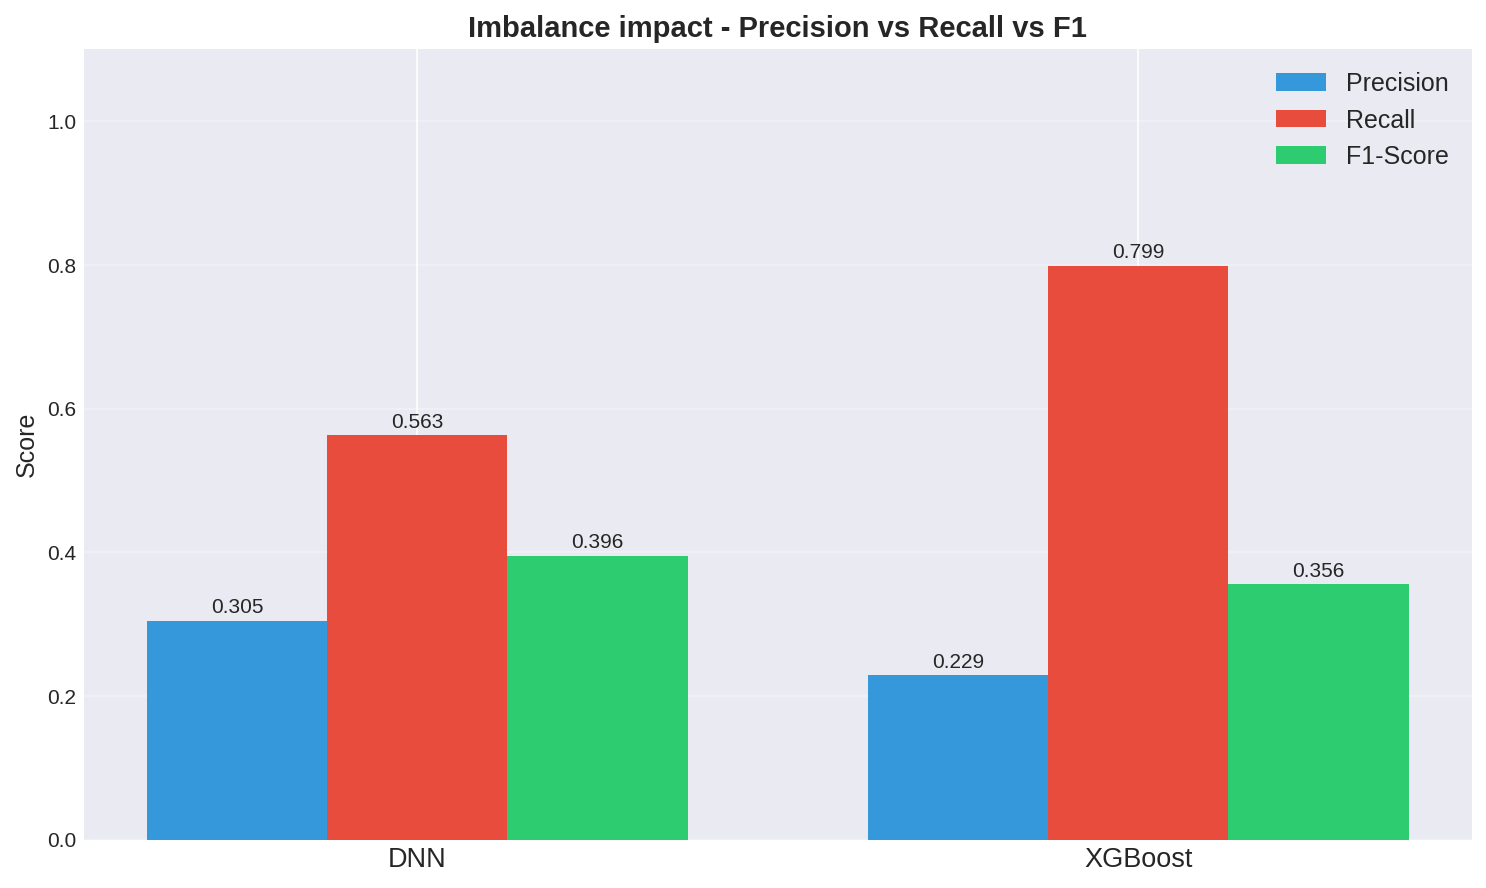
\includegraphics[width=0.85\linewidth]{figures/class_imbalance_analysis.png}
  \caption{Analyse du déséquilibre de classes du dataset BRFSS 2020--2024
           (10,32\,\% de cas positifs, rapport 8,7~:~1)}
  \label{fig:distrib_classes}
\end{figure}

% ─────────────────────────────────────────────────────────────────────────────
\section{Architecture du modèle DNN proposé}
% ─────────────────────────────────────────────────────────────────────────────

\subsection{Conception du réseau DNN}

Le modèle \acs{DNN} développé dans notre approche s'appuie sur une architecture
multicouche entièrement connectée, adaptée aux données tabulaires structurées du
dataset \acs{BRFSS}. Il comporte trois couches cachées de tailles décroissantes
(256 $\rightarrow$ 128 $\rightarrow$ 64 neurones) suivies d'une couche de sortie
sigmoïde. Des couches de \textit{Batch Normalization} et de \textit{Dropout} (taux
0,30) sont intercalées entre les premières couches pour stabiliser l'entraînement
et prévenir le surapprentissage. Le détail de cette architecture et le rôle de
chaque couche sont présentés au chapitre~\ref{chap:impl}.

\subsection{Stratégie d'entraînement}

Le prétraitement étant distribué sur les trois workers Spark, l'entraînement du
\acs{DNN} s'effectue ensuite sur le jeu de données consolidé. La configuration
d'apprentissage adoptée est la suivante :

\begin{itemize}
  \item \textbf{Optimiseur :} Adam avec un taux d'apprentissage initial
    \texttt{lr = 1e-3} ;
  \item \textbf{Fonction de perte :} entropie croisée binaire, pondérée par les
    \textit{class weights} pour compenser le déséquilibre ;
  \item \textbf{Arrêt précoce (\textit{EarlyStopping}) :} l'entraînement est
    interrompu lorsque l'AUC de validation cesse de progresser (patience de 5
    époques), avec restauration des meilleurs poids ;
  \item \textbf{Réduction adaptative du taux d'apprentissage
    (\textit{ReduceLROnPlateau}) :} division par deux du taux d'apprentissage en cas
    de stagnation, jusqu'à un minimum de \texttt{1e-6}.
\end{itemize}

\subsection{Optimisation du seuil de décision}

Avec une pondération de classes élevée, le modèle produit des probabilités
systématiquement plus hautes pour la classe positive~; le seuil par défaut de 0,5
n'est alors plus optimal. Le seuil de décision $\tau^\star$ est donc déterminé
\textit{a posteriori} en maximisant le F1-score sur la courbe Précision--Rappel
calculée sur le jeu de test. Cette étape permet d'ajuster le compromis entre
sensibilité (rappel) et précision selon l'usage clinique visé — dépistage ou
confirmation diagnostique.

% ─────────────────────────────────────────────────────────────────────────────
\section{Modèle de référence (benchmark) : XGBoost}
% ─────────────────────────────────────────────────────────────────────────────

Afin d'évaluer objectivement les performances de notre modèle \acs{DNN} distribué,
il est indispensable de le confronter à un modèle de référence (\textit{benchmark})
solide et reconnu. Nous avons retenu à cet effet l'algorithme \acf{XGBoost}, qui
constitue aujourd'hui l'état de l'art pour la classification sur données tabulaires
structurées \cite{chen2016}.

\subsection{Principe de l'algorithme XGBoost}

\acs{XGBoost} est une implémentation optimisée du \textbf{boosting de gradient}
(\textit{gradient boosting}). Le principe consiste à construire une séquence d'arbres
de décision peu profonds, où chaque nouvel arbre est entraîné pour corriger les
erreurs résiduelles commises par l'ensemble des arbres précédents. La prédiction
finale résulte de la somme pondérée des prédictions de tous les arbres. \acs{XGBoost}
enrichit ce schéma de plusieurs optimisations : une régularisation $L_1$ et $L_2$
limitant le surapprentissage, une gestion native des valeurs manquantes, et une
parallélisation efficace de la construction des arbres.

\subsection{Rôle de XGBoost dans la comparaison}

Dans notre démarche, \acs{XGBoost} n'est pas le modèle final retenu mais un
\textbf{point de comparaison} permettant de situer la valeur ajoutée de l'approche
\acs{DNN} distribuée. Il est entraîné sur le \textbf{même jeu de données prétraité}
et évalué sur le \textbf{même ensemble de test} que le \acs{DNN}, garantissant ainsi
une comparaison équitable. Le paramètre \texttt{scale\_pos\_weight} y joue le rôle
des poids de classes, compensant le déséquilibre de la variable cible. Les métriques
obtenues par \acs{XGBoost} (précision, rappel, F1-score et \acs{AUC}) servent de
référence pour juger si le surcoût computationnel d'un réseau de neurones profond
distribué est justifié par un gain de performance prédictive. Cette mise en regard
fait l'objet d'une analyse détaillée au chapitre suivant.

\section*{Conclusion}
\addcontentsline{toc}{section}{Conclusion}

Ce troisième chapitre a présenté l'approche méthodologique adoptée, articulée
autour de la combinaison du traitement distribué Apache Spark et des architectures
\acs{DNN}, ainsi que du choix d'\acs{XGBoost} comme modèle de référence pour la
comparaison des performances. Le pipeline conçu garantit scalabilité, reproductibilité et performance
pour la prédiction des maladies cardiovasculaires sur le dataset \acs{BRFSS}
2020--2024. Le chapitre suivant présente la mise en \oe{}uvre concrète et les
résultats expérimentaux obtenus.

% ══════════════════════════════════════════════════════════════════════════════
\chapter{Implémentation et visualisation}
\label{chap:impl}
% ══════════════════════════════════════════════════════════════════════════════

\section*{Introduction}
\addcontentsline{toc}{section}{Introduction}

Ce quatrième et dernier chapitre de développement présente la mise en \oe{}uvre
concrète du pipeline de prédiction cardiovasculaire. Nous décrivons successivement
l'environnement de développement, la collecte et la préparation des données, le
pipeline détaillé du modèle \acs{DNN} et le rôle de ses différentes couches,
l'entraînement distribué et les métriques d'évaluation, puis nous analysons,
visualisons et comparons les résultats obtenus.

% ─────────────────────────────────────────────────────────────────────────────
\section{Environnement de travail}
% ─────────────────────────────────────────────────────────────────────────────

\subsection{Matériel}

Les expériences ont été conduites sur la plateforme \textbf{Kaggle Notebooks}, qui
met à disposition gratuitement des ressources \acs{GPU} adaptées à l'entraînement
de modèles profonds, ainsi qu'un accès direct au dataset \acs{BRFSS} via l'API
\texttt{kagglehub}. Les caractéristiques de l'environnement sont les suivantes :

\begin{itemize}
  \item \textbf{Plateforme :} Kaggle Notebooks (exécution en ligne) ;
  \item \textbf{Processeur :} Intel Xeon, 4 cœurs ;
  \item \textbf{Mémoire vive :} 29~Go de \acs{RAM} (mode \acs{GPU}) ;
  \item \textbf{Carte graphique :} 2 $\times$ NVIDIA Tesla T4 (13\,757~Mo de VRAM
    chacune) ;
  \item \textbf{Stockage :} 20~Go (espace de travail \texttt{/kaggle/working/}).
\end{itemize}

\subsection{Logiciels, frameworks et plateformes}

\begin{table}[H]
\centering
\caption{Bibliothèques et versions utilisées}
\label{tab:libs}
\begin{tabularx}{\textwidth}{L{5cm} C{3cm} X}
\toprule
\textbf{Bibliothèque / Outil} & \textbf{Version} & \textbf{Usage} \\
\midrule
Python         & 3.10    & Langage principal \\
Apache Spark (PySpark) & 3.5+ & Ingestion et prétraitement distribués \\
TensorFlow / Keras     & 2.19 & Modèle DNN \\
XGBoost        & 3.2     & Modèle de référence (benchmark) \\
Scikit-learn   & 1.3     & Prétraitement, métriques, class weights \\
Pandas         & 2.x     & Manipulation de données \\
NumPy          & 1.26    & Calcul numérique \\
Matplotlib / Seaborn & 3.7 / 0.12 & Visualisation \\
Streamlit      & 1.28+   & Tableau de bord interactif \\
Jupyter / Kaggle & ---   & Environnement interactif \\
\bottomrule
\end{tabularx}
\end{table}

\noindent Les figures suivantes illustrent les outils principaux utilisés dans ce projet.

\begin{figure}[H]
  \centering
  \includegraphics[width=0.3\linewidth]{figures/logoapachespark.png}
  \caption{Apache Spark -- Framework de traitement distribué}
  \label{fig:spark_logo}
\end{figure}

\noindent{\small\itshape Apache Spark est le moteur de calcul distribué employé dans
ce projet pour l'ingestion et le prétraitement à grande échelle des 2,17~millions
d'enregistrements du \acs{BRFSS}.}

\begin{figure}[H]
  \centering
  \includegraphics[width=0.2\linewidth]{figures/python.jpeg}
  \caption{Python et Jupyter Notebook -- Langage et environnement de développement}
  \label{fig:python_jupyter}
\end{figure}

\noindent{\small\itshape Python et l'environnement interactif Jupyter/Kaggle
constituent le socle de développement du pipeline, de la manipulation des données
jusqu'à l'évaluation des modèles.}

\begin{figure}[H]
  \centering
  \includegraphics[width=0.5\linewidth]{figures/logotenserflow.png}
  \caption{TensorFlow / Keras -- Framework de Deep Learning}
  \label{fig:tf_keras}
\end{figure}

\noindent{\small\itshape TensorFlow et son interface Keras ont servi à construire,
entraîner et évaluer le réseau de neurones profond (\acs{DNN}) au c\oe{}ur du
système de prédiction.}

% ─────────────────────────────────────────────────────────────────────────────
\section{Collecte et préparation des données}
% ─────────────────────────────────────────────────────────────────────────────

\subsection{Source et organisation du dataset}

Le dataset \acs{BRFSS} 2020--2024 est disponible sur la plateforme Kaggle
\cite{brfss2024kaggle}. Il est chargé au format \textbf{Parquet} (fichier poolé
\texttt{\_ml}) regroupant les cinq années d'enquête. Le chargement initial via
PySpark compte \textbf{2\,176\,776 lignes} et 129 colonnes brutes. Après
binarisation au format BRFSS (codes $1=$Oui$/2=$Non recodés en $0/1$), dérivation de
la cible \texttt{HeartDiseaseorAttack} à partir de la variable composite
\texttt{\_MICHD}, sélection des 14 variables pertinentes et suppression de
\textbf{416\,535 doublons}, le jeu de données nettoyé compte \textbf{1\,760\,241
observations} avec une prévalence de 10,32\,\% de cas positifs. La variable cible
est binaire (0 : pas de maladie, 1 : cardiopathie coronarienne ou infarctus).

\begin{table}[H]
\centering
\caption{Présentation d’un extrait du dataset BRFSS 2020--2024}
\label{tab:kaggle_dataset}

\renewcommand{\arraystretch}{1.2}

\resizebox{\textwidth}{!}{
\begin{tabular}{|c|c|c|c|c|c|c|c|c|c|}
\hline
\textbf{\_STATE} & \textbf{FMONTH} & \textbf{IDATE} & \textbf{IMONTH} &
\textbf{IDAY} & \textbf{IYEAR} & \textbf{DISPCODE} &
\textbf{SEQNO} & \textbf{\_PSU} & \textbf{CTELENM1} \\
\hline

1.0 & 2.0 & 02282024 & 02 & 28 & 2024 & 1100.0 &
2024000001 & $2.024\times10^9$ & 1.0 \\
\hline

1.0 & 2.0 & 02212024 & 02 & 21 & 2024 & 1100.0 &
2024000002 & $2.024\times10^9$ & 1.0 \\
\hline

1.0 & 2.0 & 02212024 & 02 & 21 & 2024 & 1100.0 &
2024000003 & $2.024\times10^9$ & 1.0 \\
\hline

1.0 & 2.0 & 02282024 & 02 & 28 & 2024 & 1100.0 &
2024000004 & $2.024\times10^9$ & 1.0 \\
\hline

1.0 & 2.0 & 02212024 & 02 & 21 & 2024 & 1100.0 &
2024000005 & $2.024\times10^9$ & 1.0 \\
\hline

\end{tabular}
}

\vspace{0.3cm}

\small
Source : Extrait du dataset BRFSS utilisé pour l’analyse des maladies cardiovasculaires.

\end{table}

\subsection{Prétraitement et analyse exploratoire}

Après le prétraitement distribué décrit au chapitre précédent (imputation par la
médiane pour les variables continues et par le mode pour les variables
catégorielles, normalisation par \texttt{StandardScaler}), une analyse exploratoire
est conduite. La figure~\ref{fig:distrib} confirme le déséquilibre de la variable
cible, et la figure~\ref{fig:mcv_age} valide la cohérence épidémiologique des
données : la prévalence des \acs{MCV} croît de façon strictement monotone avec
l'âge, de 0,9\,\% chez les 18--24~ans à 24,7\,\% chez les 80~ans et plus.

\begin{figure}[H]
  \centering
  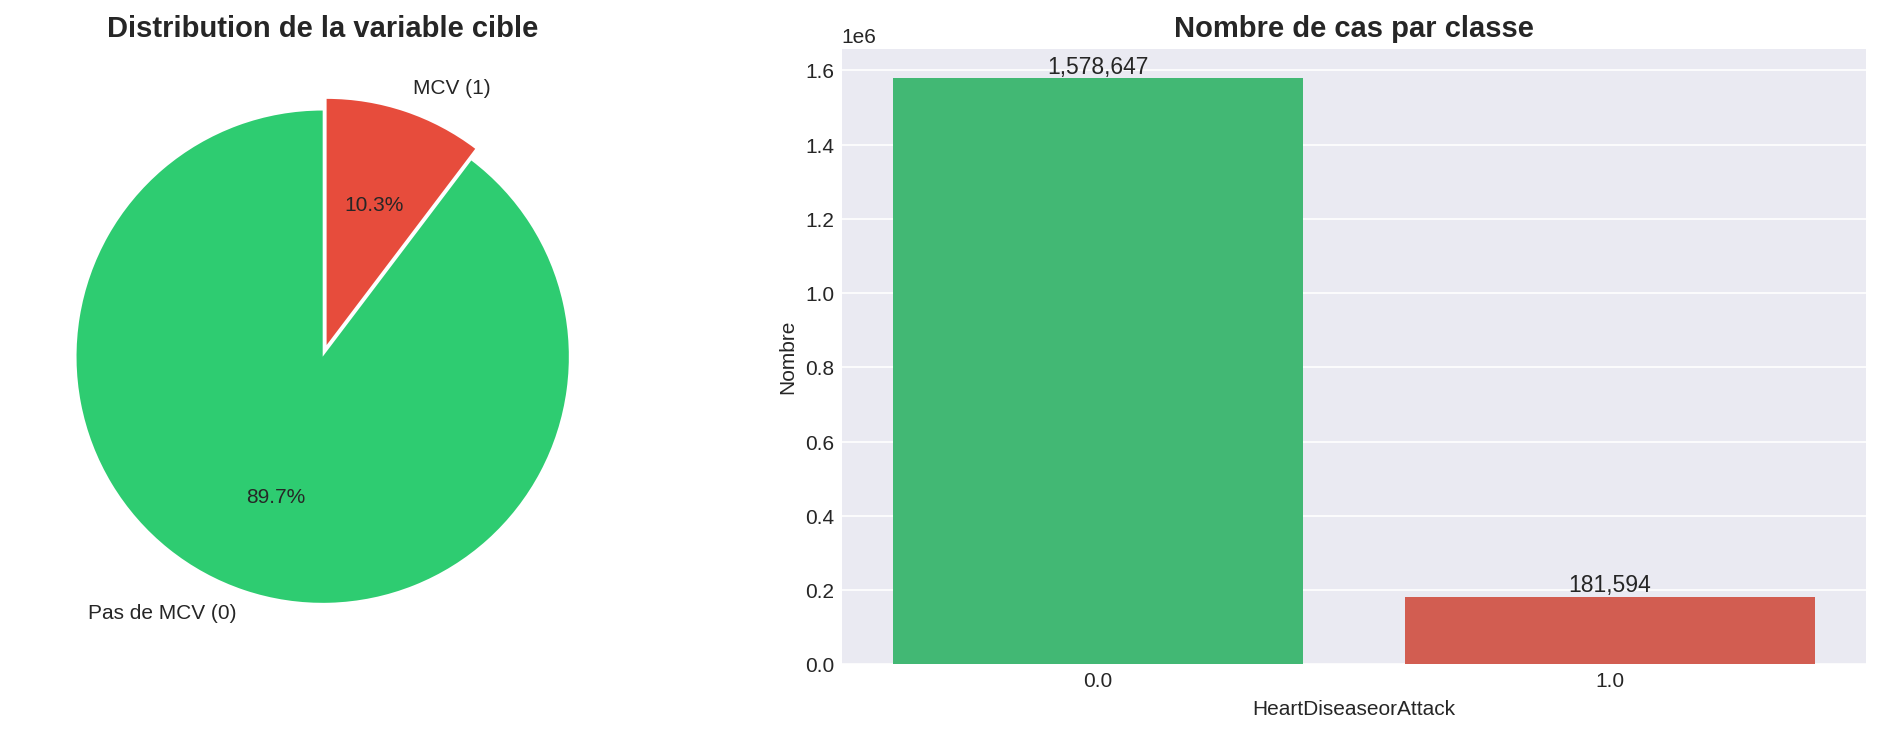
\includegraphics[width=0.85\linewidth]{figures/target_distribution.png}
  \caption{Distribution de la variable cible \texttt{HeartDiseaseorAttack}
           (1\,760\,241 observations, 10,32\,\% de cas positifs)}
  \label{fig:distrib}
\end{figure}

\noindent{\small\itshape Cet histogramme illustre le fort déséquilibre de la variable
cible : la classe « non malade » représente 89,68\,\% des observations contre seulement
10,32\,\% de cas positifs, justifiant le recours à la pondération des classes.}

\begin{figure}[H]
  \centering
  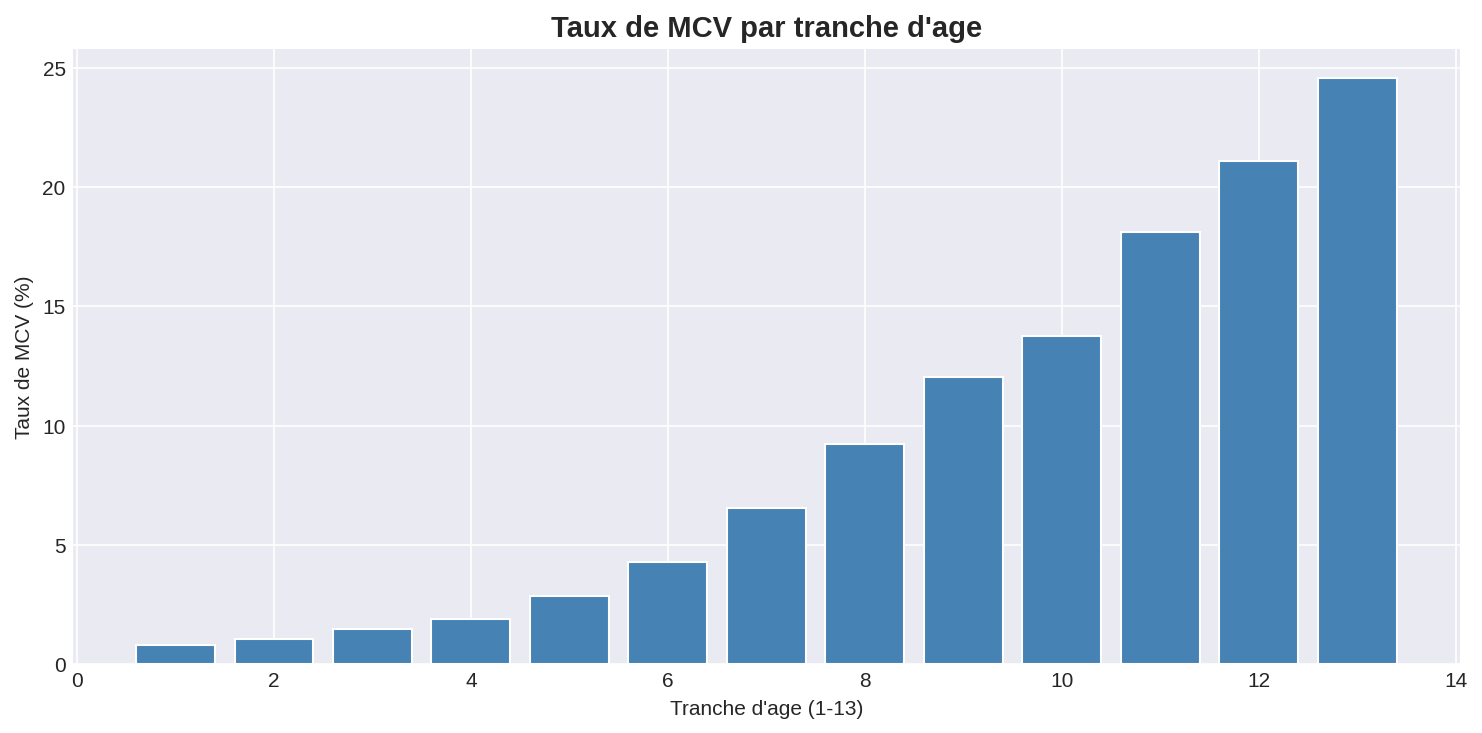
\includegraphics[width=0.92\linewidth]{figures/mcv_by_age.png}
  \caption{Taux de MCV par tranche d'âge --- progression monotone validant
           la cohérence du pipeline de binarisation}
  \label{fig:mcv_age}
\end{figure}

\noindent{\small\itshape La prévalence des \acs{MCV} croît de manière strictement
monotone avec l'âge, passant de 0,9\,\% chez les 18--24~ans à 24,7\,\% chez les
80~ans et plus, ce qui confirme la validité épidémiologique des données prétraitées.}

La matrice de corrélation (figure~\ref{fig:corr}) met en évidence les variables les
plus liées à la cible : \texttt{Age} (0,250), \texttt{GenHlth} (0,213),
\texttt{Stroke} (0,188) et \texttt{DiffWalk} (0,183), tandis que l'activité physique
présente une corrélation négative (effet protecteur).

\begin{figure}[H]
  \centering
  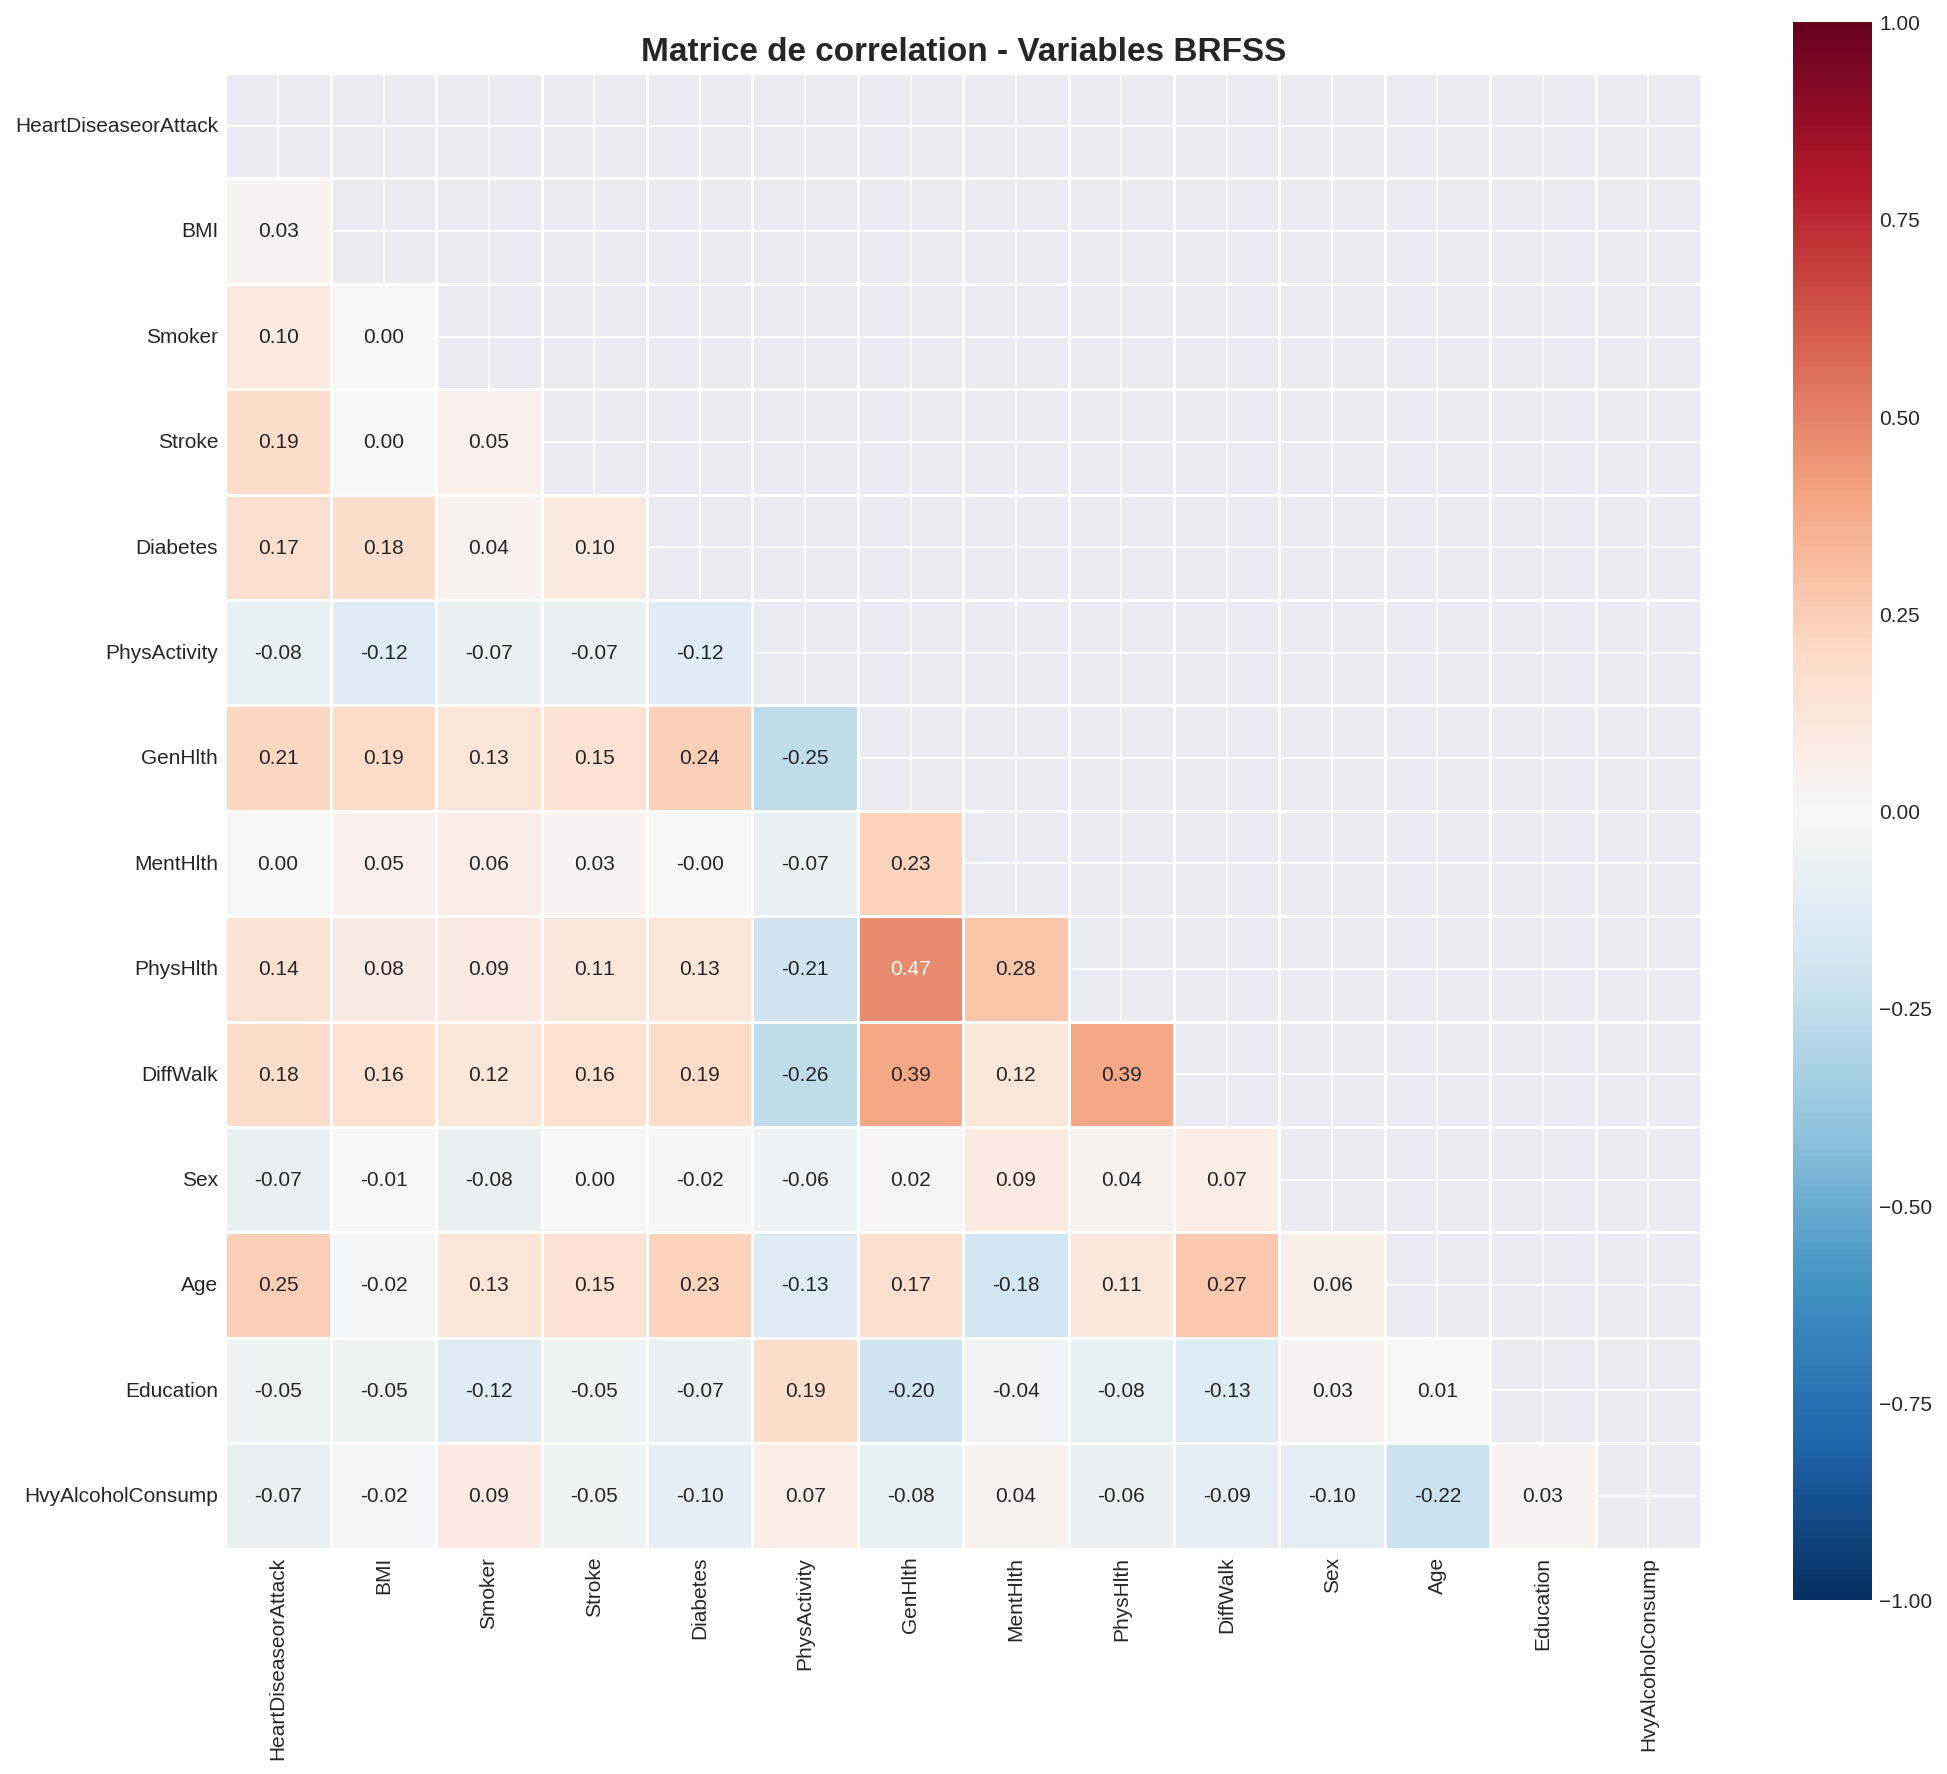
\includegraphics[width=\linewidth]{figures/correlation_heatmap.png}
  \caption{Matrice de corrélation de Pearson des variables du dataset BRFSS
           (échantillon de 200\,000 lignes)}
  \label{fig:corr}
\end{figure}

\noindent{\small\itshape Les cases les plus foncées mettent en évidence les variables
les plus corrélées à la cible --- \texttt{Age}, \texttt{GenHlth}, \texttt{Stroke} et
\texttt{DiffWalk} --- tandis que l'activité physique présente une corrélation négative,
traduisant un effet protecteur.}

\subsection{Sélection des variables et features dérivées}

La pertinence des variables est évaluée par trois méthodes complémentaires :
corrélation (Pearson/Spearman), importance de Gini (forêt aléatoire) et test du
$\chi^2$ (V de Cramér). La convergence des trois méthodes (figure~\ref{fig:gini})
désigne \texttt{Age}, \texttt{GenHlth} et \texttt{Stroke} comme les trois variables
les plus prédictives, représentant à elles seules 70,5\,\% de l'importance totale.

\begin{figure}[H]
  \centering
  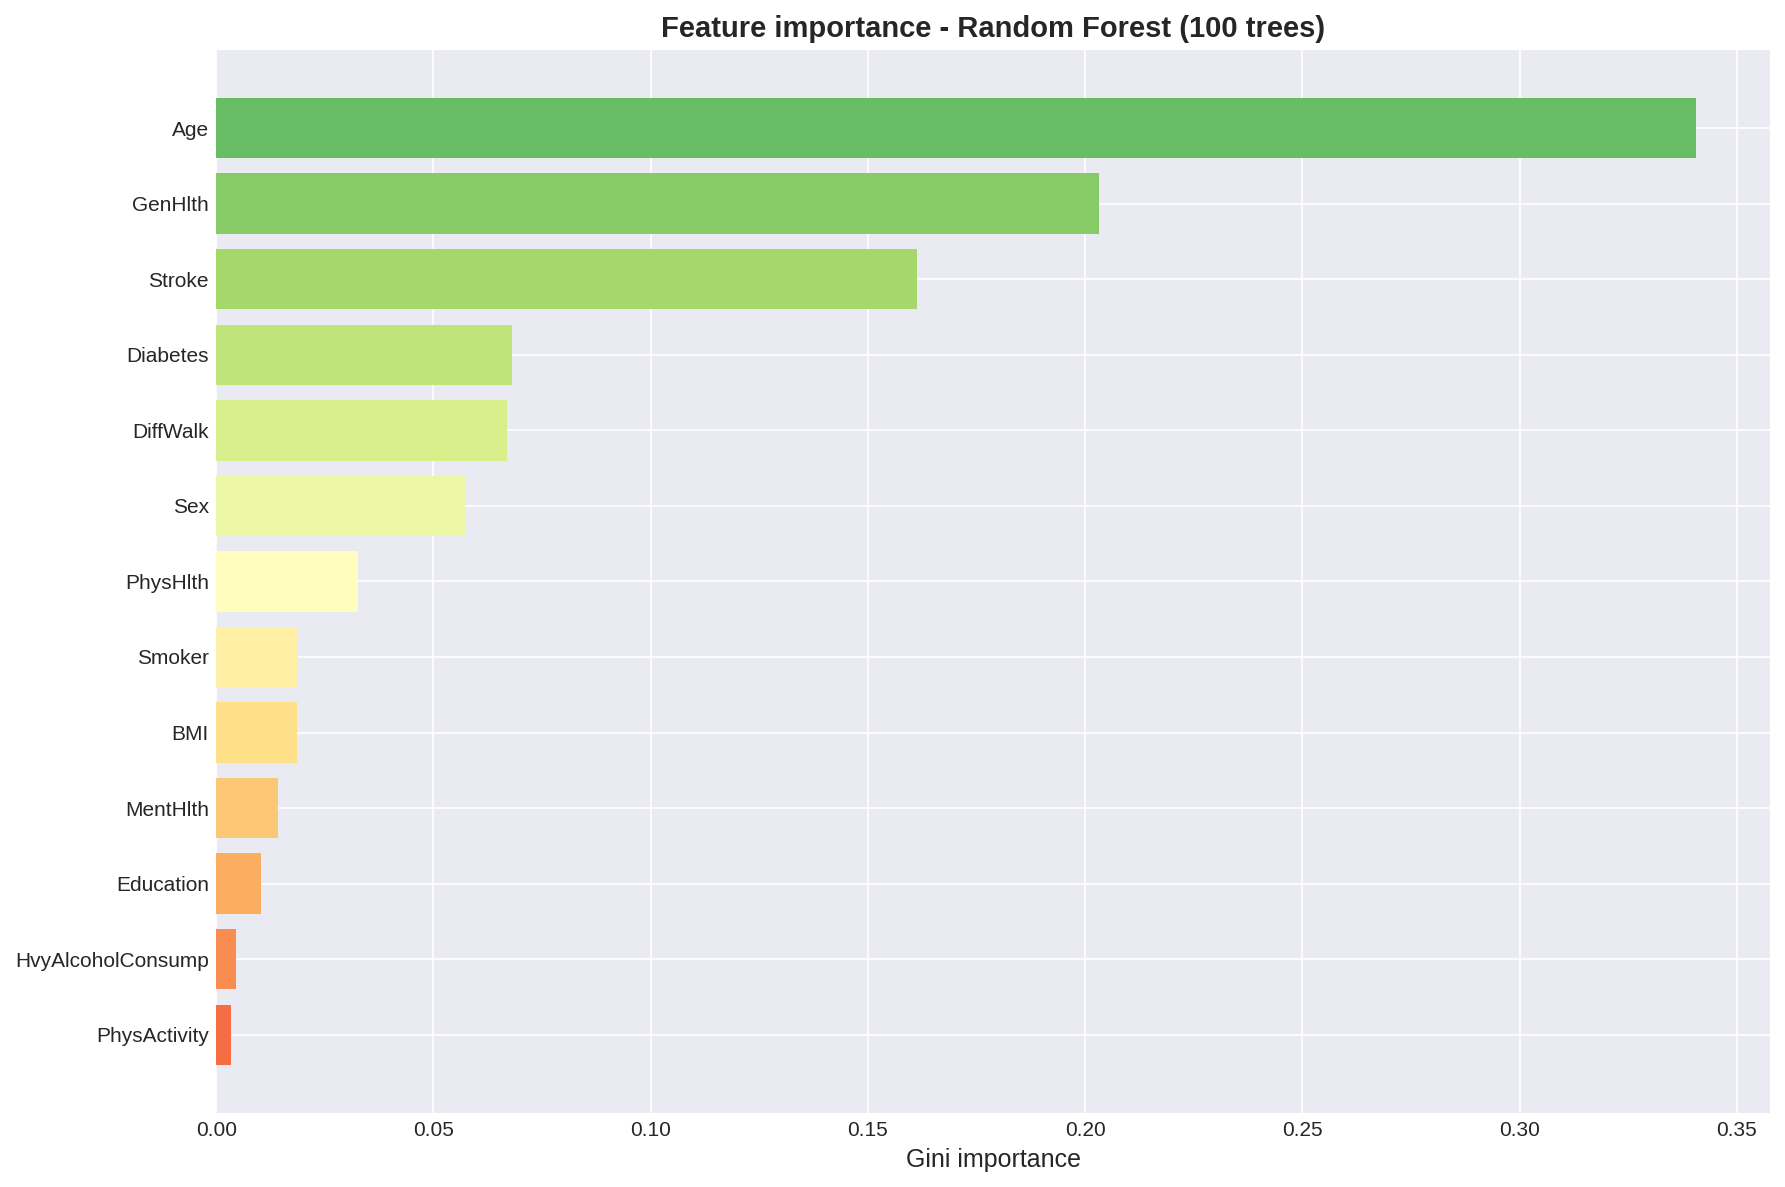
\includegraphics[width=\linewidth]{figures/feature_importance_gini.png}
  \caption{Importance des variables par réduction d'impureté de Gini
           (forêt aléatoire, 100 arbres)}
  \label{fig:gini}
\end{figure}

\noindent{\small\itshape Le diagramme classe les variables par pouvoir prédictif :
\texttt{Age}, \texttt{GenHlth} et \texttt{Stroke} se détachent nettement et
concentrent à elles seules 70,5\,\% de l'importance totale.}

Deux variables composites sont par ailleurs construites pour enrichir le signal :
le \texttt{RiskScore} (somme des facteurs de risque binaires disponibles) et
le \texttt{HealthIndex} (état de santé global normalisé). Leur distribution selon
la classe cible (figure~\ref{fig:derived}) montre une séparation nette entre les
groupes MCV et non-MCV.

\begin{figure}[H]
  \centering
  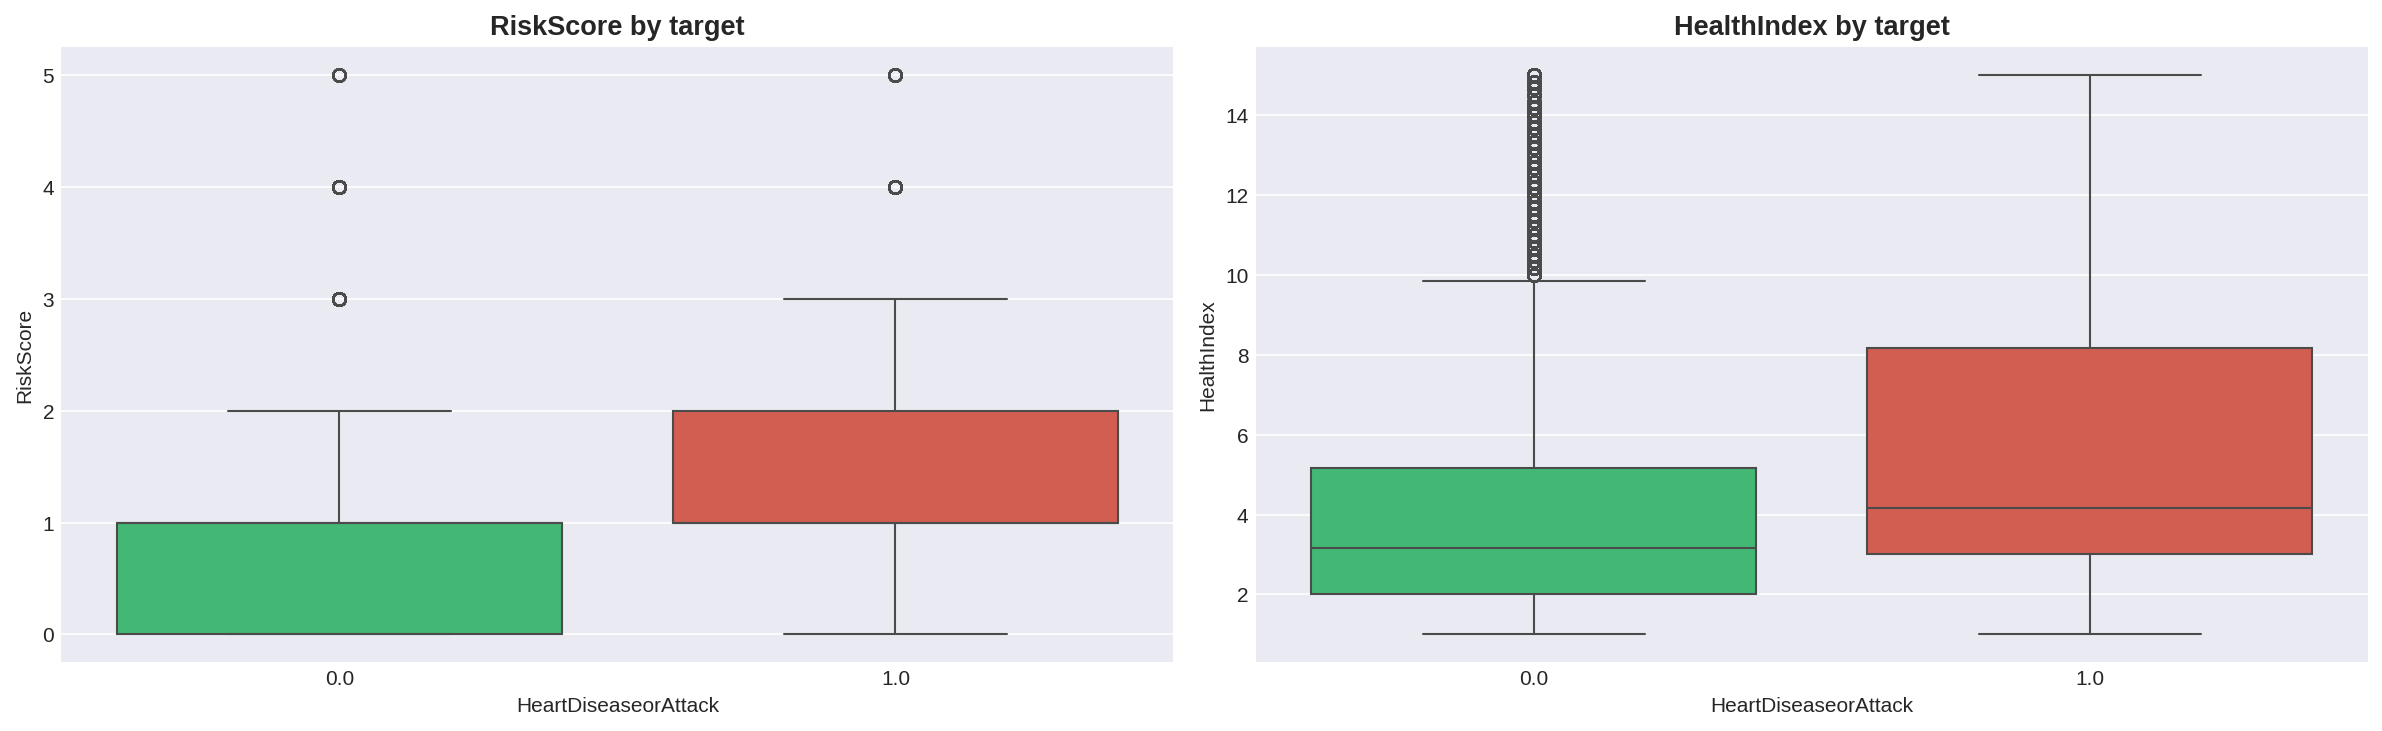
\includegraphics[width=\linewidth]{figures/derived_features.png}
  \caption{Distribution des variables dérivées \texttt{RiskScore} et
           \texttt{HealthIndex} selon la classe cible}
  \label{fig:derived}
\end{figure}

\noindent{\small\itshape Les distributions des deux variables composites se séparent
nettement entre les groupes MCV et non-MCV, ce qui confirme leur apport discriminant
au modèle de prédiction.}

\subsection{Partitionnement et normalisation}

Le jeu de données est divisé selon un schéma stratifié \textbf{70~\% / 15~\% / 15~\%}
(entraînement / validation / test), la prévalence de 10,32\,\% étant maintenue dans
chaque partition. La graine aléatoire est fixée à 42 pour la reproductibilité. Le
\texttt{StandardScaler} est ajusté \textbf{exclusivement sur l'ensemble
d'entraînement}, puis appliqué aux ensembles de validation et de test, afin de
prévenir toute fuite de données (\textit{data leakage}).

% ─────────────────────────────────────────────────────────────────────────────
\section{Entraînement du modèle DNN}
% ─────────────────────────────────────────────────────────────────────────────

Le prétraitement à grande échelle étant pris en charge de manière distribuée par
Apache Spark (cf.\ chapitre~3), l'entraînement du \acs{DNN} est ensuite réalisé sur
le jeu de données consolidé, en exploitant l'accélération des deux \acs{GPU}
Tesla~T4. L'entraînement s'est déroulé sur \textbf{36 époques} (taille de lot
1\,024), le meilleur modèle ayant été obtenu à l'\textbf{époque 31}
(val\_auc $= 0{,}8205$), pour un temps total de \textbf{177,8~secondes}. Les
courbes d'apprentissage (présentées plus loin) confirment l'absence de
surapprentissage grâce à la combinaison Dropout, Batch Normalization et arrêt
précoce.

% ─────────────────────────────────────────────────────────────────────────────
\section{Architecture du modèle DNN}
% ─────────────────────────────────────────────────────────────────────────────

\subsection{Structure détaillée du réseau}

\begin{table}[H]
\centering
\caption{Architecture détaillée du modèle DNN}
\label{tab:dnn_arch}
\begin{tabularx}{\textwidth}{C{2cm} L{3cm} C{2.5cm} C{2cm} X}
\toprule
\textbf{Couche} & \textbf{Type} & \textbf{Neurones} & \textbf{Activation} & \textbf{Régularisation} \\
\midrule
Entrée & --- & 15 features & --- & --- \\
1 & Dense          & 256    & ReLU    & BatchNorm + Dropout(0.3), $L_2 = 10^{-4}$ \\
2 & Dense          & 128    & ReLU    & BatchNorm + Dropout(0.3), $L_2 = 10^{-4}$ \\
3 & Dense          & 64     & ReLU    & --- \\
4 & Dense (sortie) & 1      & Sigmoid & --- \\
\bottomrule
\end{tabularx}
\end{table}

\noindent Le modèle totalise 46\,849 paramètres (dont 46\,081 entraînables). Les
15~\textit{features} d'entrée correspondent aux 13 variables retenues à l'issue de la
sélection, augmentées des deux variables dérivées \texttt{RiskScore} et
\texttt{HealthIndex}.

\subsection{Pipeline du modèle DNN}

Le modèle \acs{DNN} s'inscrit dans un pipeline complet allant de la donnée brute à
la prédiction du risque cardiovasculaire. Ce pipeline enchaîne les étapes suivantes :

\begin{enumerate}
  \item \textbf{Entrée des données :} le vecteur des caractéristiques prétraitées
    (variables normalisées et encodées issues du prétraitement Spark) est présenté à
    la couche d'entrée du réseau ;
  \item \textbf{Extraction hiérarchique de caractéristiques :} les couches cachées
    successives (256 $\rightarrow$ 128 $\rightarrow$ 64 neurones)
    transforment progressivement ces variables en représentations de plus en plus
    abstraites, capturant les interactions non linéaires entre facteurs de risque ;
  \item \textbf{Décision :} la couche de sortie produit une probabilité d'appartenance
    à la classe \og malade \fg{} ;
  \item \textbf{Seuillage et évaluation :} cette probabilité est comparée à un seuil
    de décision pour produire la classe finale, puis confrontée à la vérité terrain
    pour le calcul des métriques.
\end{enumerate}

La figure~\ref{fig:dnn_pipeline} illustre l'enchaînement de ces couches, depuis le
vecteur d'entrée jusqu'à la probabilité de sortie.

\begin{figure}[H]
  \centering
  \includegraphics[width=\linewidth]{figures/dnn_arch.png}
  \caption{Pipeline complet du modèle DNN, de l'entrée à la prédiction}
  \label{fig:dnn_pipeline}
\end{figure}

\noindent{\small\itshape Le schéma retrace le cheminement d'un patient dans le réseau :
le vecteur d'entrée traverse les couches denses décroissantes
(256~$\rightarrow$~128~$\rightarrow$~64) avant la couche sigmoïde qui produit la
probabilité d'être atteint d'une maladie cardiovasculaire.}

\subsection{Rôle et fonctionnement des différentes couches}

Chaque type de couche du réseau remplit une fonction précise dans le processus
d'apprentissage et de prédiction :

\begin{itemize}
  \item \textbf{Couche d'entrée (\textit{Input Layer}) :} elle reçoit le vecteur des
    caractéristiques (âge, BMI, hypertension, diabète, etc.) et ne réalise aucun
    calcul ; sa dimension est fixée par le nombre de variables explicatives.

  \item \textbf{Couches denses (\textit{Fully Connected}) :} c\oe{}ur du réseau,
    chaque neurone y est connecté à tous les neurones de la couche précédente et
    calcule une somme pondérée de ses entrées augmentée d'un biais
    ($z = \sum_i w_i x_i + b$). Les poids $w_i$ sont les paramètres appris durant
    l'entraînement. La réduction progressive du nombre de neurones
    (256 $\rightarrow$ 32) force le réseau à compresser l'information vers les
    représentations les plus discriminantes.

  \item \textbf{Fonction d'activation ReLU :} appliquée en sortie de chaque couche
    cachée, la fonction $f(x)=\max(0,x)$ introduit la \textbf{non-linéarité}
    indispensable pour modéliser des relations complexes entre facteurs de risque.
    Sans elle, l'empilement de couches denses se réduirait à une simple transformation
    linéaire. ReLU présente en outre l'avantage d'atténuer le problème de disparition
    du gradient et d'accélérer la convergence.

  \item \textbf{Batch Normalization :} insérée après les premières couches denses,
    elle normalise les activations de chaque lot (moyenne nulle, variance unitaire).
    Elle stabilise et accélère l'entraînement en limitant le décalage de la
    distribution des activations (\textit{internal covariate shift}) et exerce un
    léger effet régularisant.

  \item \textbf{Dropout :} cette couche désactive aléatoirement une fraction des
    neurones (taux de 30\,\%) à chaque itération d'entraînement. En empêchant le
    réseau de trop s'appuyer sur des neurones spécifiques, elle réduit le
    surapprentissage et améliore la capacité de généralisation du modèle sur des
    patients non vus.

  \item \textbf{Couche de sortie (\textit{Sigmoid}) :} composée d'un unique neurone,
    elle applique la fonction sigmoïde $f(x)=\frac{1}{1+e^{-x}}$ qui comprime la
    sortie dans l'intervalle $[0,1]$, interprétable directement comme la
    \textbf{probabilité} qu'un patient soit atteint d'une maladie cardiovasculaire.
\end{itemize}

% ─────────────────────────────────────────────────────────────────────────────
\section{Métriques d'évaluation}
% ─────────────────────────────────────────────────────────────────────────────

Compte tenu du contexte médical et du déséquilibre de classes, les métriques
retenues pour l'évaluation sont :

\subsection{Précision globale (Accuracy)}

Mesure le pourcentage d'instances correctement prédites :
\[
\text{Accuracy} = \frac{VP + VN}{VP + VN + FP + FN}
\]

\subsection{Précision (Precision)}

Indique combien d'instances prédites comme positives sont réellement positives :
\[
\text{Precision} = \frac{VP}{VP + FP}
\]

\subsection{Rappel (Recall / Sensibilité)}

Proportion de vrais malades correctement identifiés --- métrique prioritaire en
contexte médical :
\[
\text{Recall} = \frac{VP}{VP + FN}
\]

\subsection{Score F1}

Moyenne harmonique de la précision et du rappel :
\[
\text{F1} = 2 \times \frac{\text{Precision} \times \text{Recall}}{\text{Precision} + \text{Recall}}
\]

\subsection{AUC-ROC}

Surface sous la courbe \acs{ROC}, mesure globale de la capacité discriminante du
modèle indépendante du seuil de classification.

\subsection{Matrice de confusion}

La matrice de confusion est un tableau visualisant les performances du modèle en
affichant le nombre de vrais positifs (VP), vrais négatifs (VN), faux positifs (FP)
et faux négatifs (FN).

% ─────────────────────────────────────────────────────────────────────────────
\section{Résultats expérimentaux}
% ─────────────────────────────────────────────────────────────────────────────

\subsection{Configuration et résumé de l'entraînement}

Le tableau~\ref{tab:executions} récapitule la configuration et les résultats de
l'entraînement du modèle \acs{DNN}, évalué au seuil par défaut (0,5) et au seuil
optimal (0,6713) déterminé par maximisation du F1-score.

\begin{table}[H]
\centering
\caption{Configuration et résultats de l'entraînement du DNN}
\label{tab:executions}
\begin{tabularx}{\textwidth}{L{6cm} X}
\toprule
\textbf{Paramètre} & \textbf{Valeur} \\
\midrule
Architecture                 & 256--128--64--1 (46\,849 paramètres) \\
Optimiseur / taux d'apprentissage & Adam / $10^{-3}$ \\
Taille de lot / époques max   & 1\,024 / 50 \\
Époques effectuées (meilleure) & 36 (époque 31) \\
Gestion du déséquilibre       & Class weights $\{0:0{,}558\,;\,1:4{,}847\}$ \\
Temps d'entraînement          & 177,8~s (2 $\times$ Tesla T4) \\
Meilleur val\_auc             & 0,8205 \\
\midrule
AUC-ROC (test)                & 0,819 \\
Recall / F1 (seuil 0,5)       & 0,802 / 0,354 \\
Recall / F1 (seuil 0,6713)    & 0,563 / 0,396 \\
\bottomrule
\end{tabularx}
\end{table}

\subsection{Performances du modèle DNN}

\subsubsection{Courbes d'apprentissage}

Les courbes d'apprentissage (figure~\ref{fig:dnn_lc}) montrent que l'AUC de validation
dépasse 0,82 dès la première époque et n'évolue ensuite que faiblement
($+0{,}003$ sur 36 époques). La convergence parallèle des courbes d'entraînement et
de validation confirme l'\textbf{absence de surapprentissage}. Ce plateau précoce
indique que la limite de performance est imposée par l'information contenue dans les
variables disponibles, et non par la capacité du réseau.

\begin{figure}[H]
  \centering
  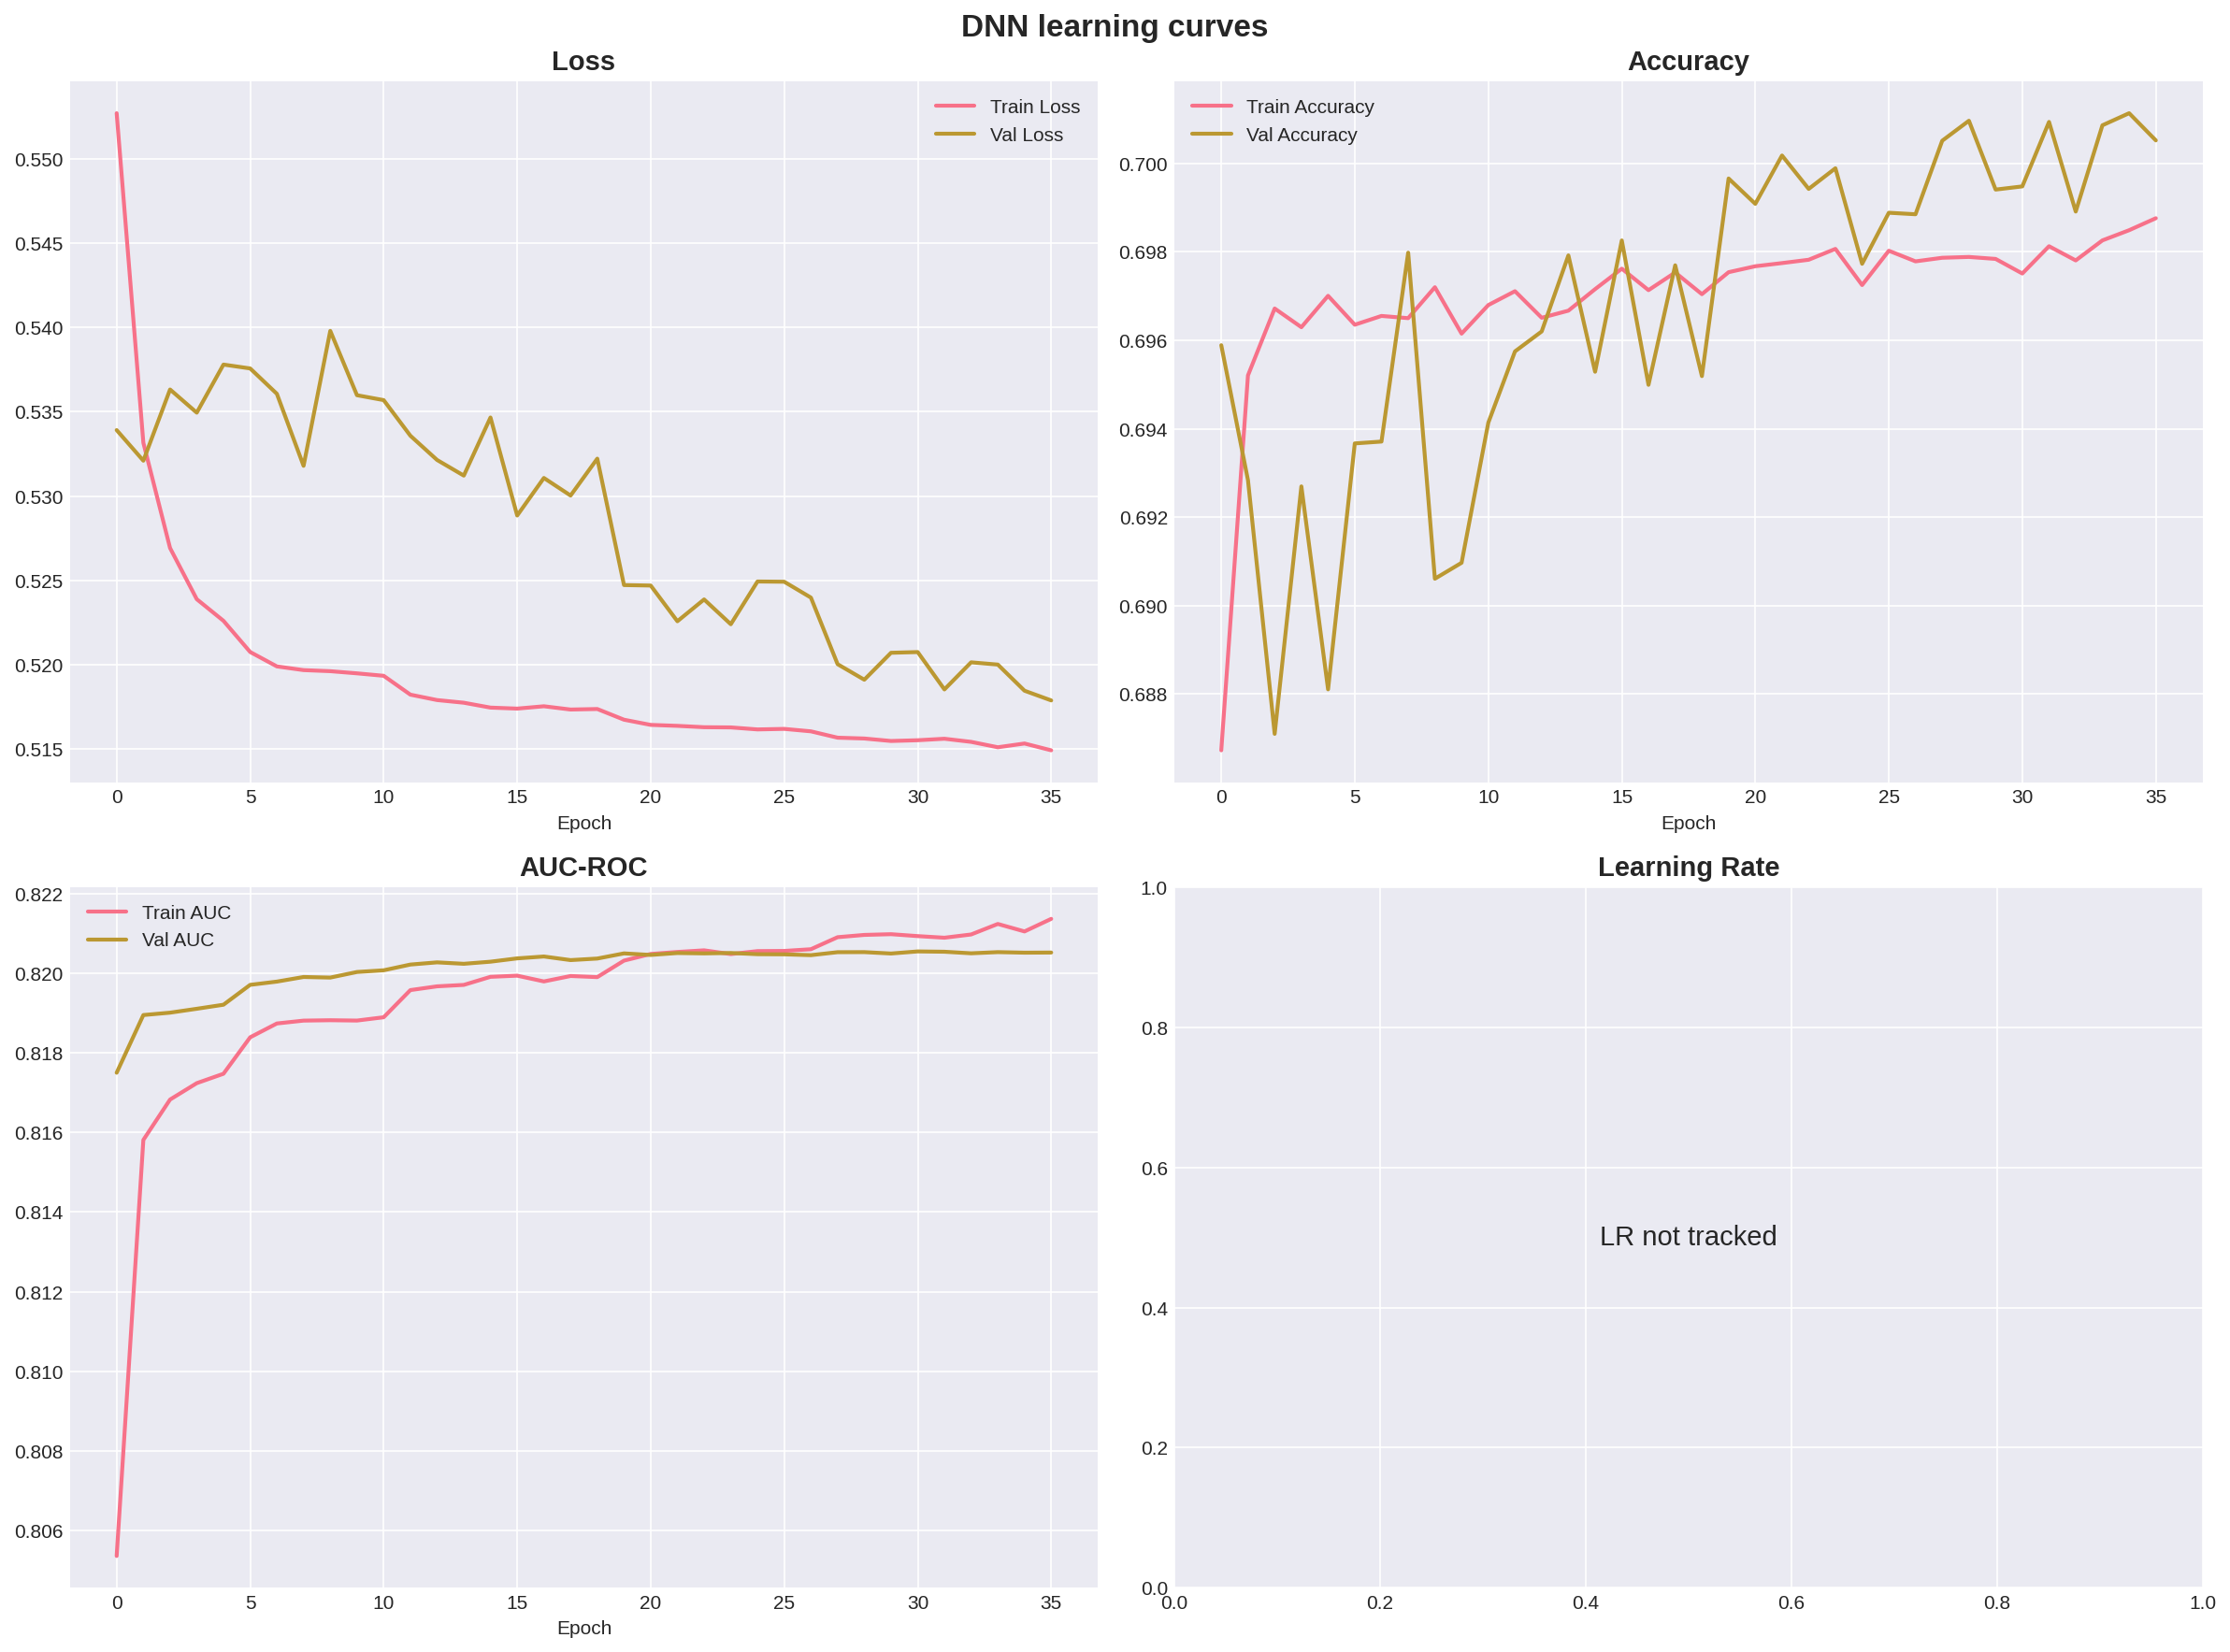
\includegraphics[width=\linewidth]{figures/dnn_learning_curves.png}
  \caption{Courbes d'apprentissage du DNN --- perte (gauche) et AUC (droite)
           sur les ensembles d'entraînement et de validation}
  \label{fig:dnn_lc}
\end{figure}

\noindent{\small\itshape L'évolution parallèle des courbes d'entraînement et de
validation, sans divergence, atteste de l'absence de surapprentissage~; l'AUC de
validation atteint son plateau (~0,82) dès les premières époques.}

\subsubsection{Courbe ROC et matrice de confusion}

\begin{figure}[H]
  \centering
  \begin{subfigure}[b]{0.48\textwidth}
    \centering
    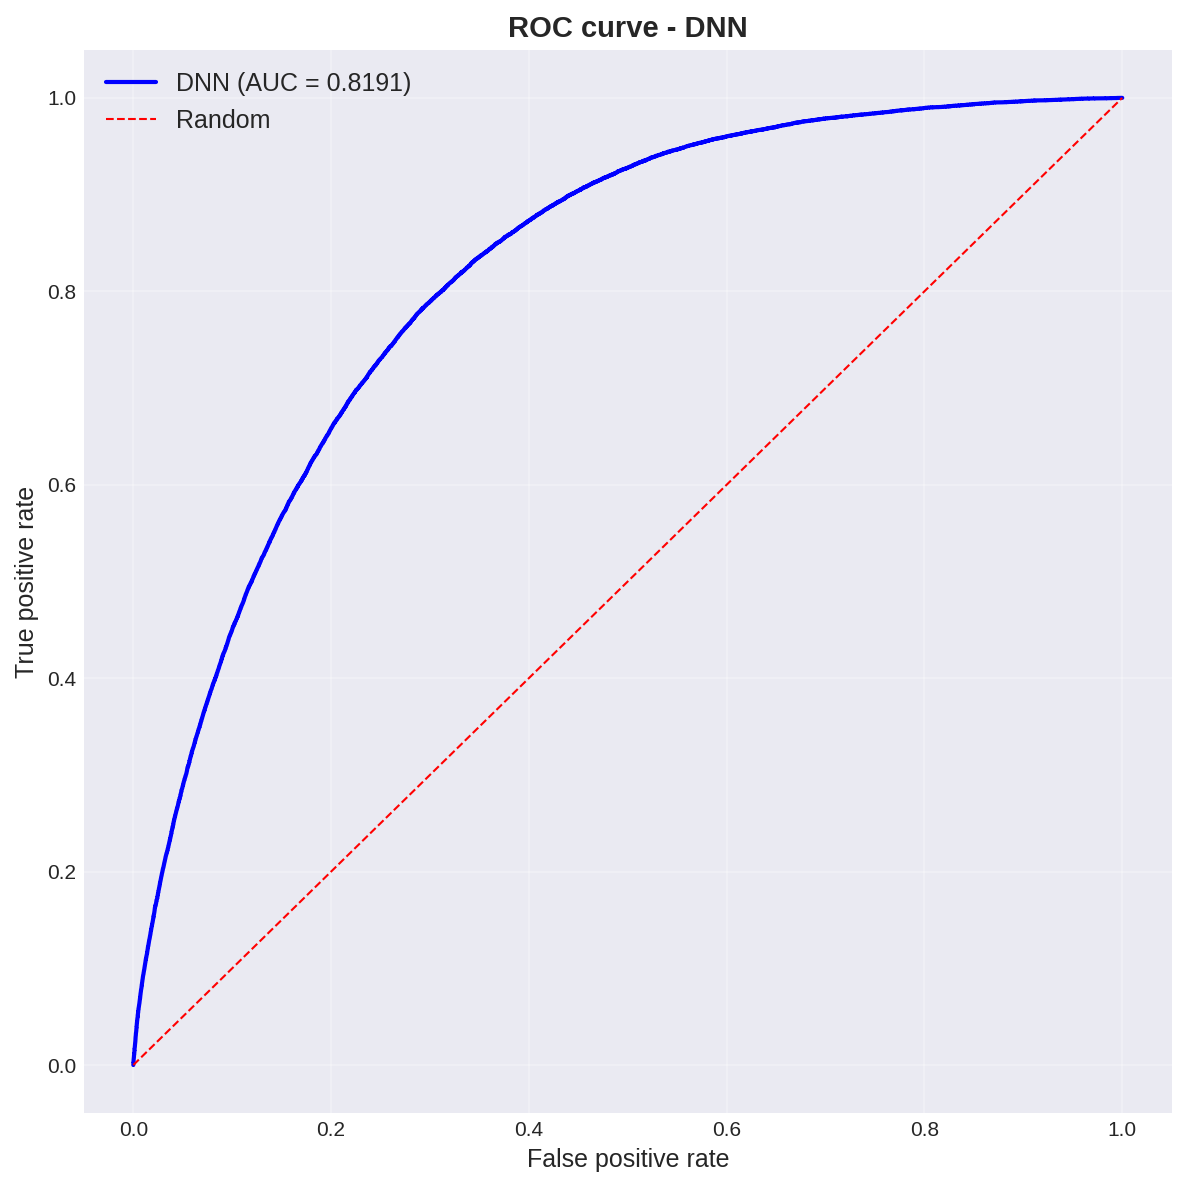
\includegraphics[width=\textwidth]{figures/dnn_roc_curve.png}
    \caption{Courbe ROC (AUC = 0,819)}
    \label{fig:dnn_roc}
  \end{subfigure}
  \hfill
  \begin{subfigure}[b]{0.48\textwidth}
    \centering
    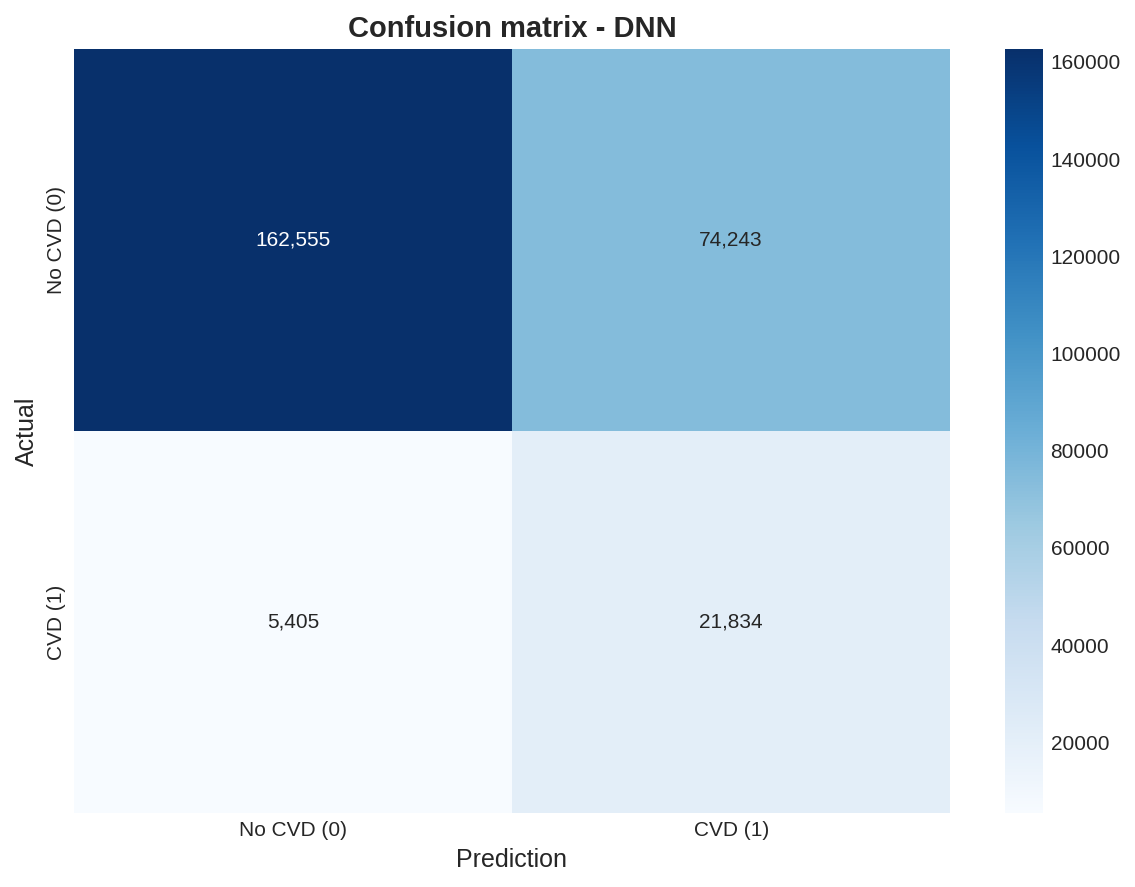
\includegraphics[width=\textwidth]{figures/dnn_confusion_matrix.png}
    \caption{Matrice de confusion (seuil 0,6713)}
    \label{fig:dnn_cm}
  \end{subfigure}
  \caption{Résultats du DNN : courbe ROC et matrice de confusion. Au seuil optimal,
           15\,333 vrais positifs sont correctement détectés contre 11\,906 faux
           négatifs.}
  \label{fig:dnn_results}
\end{figure}

\noindent{\small\itshape À gauche, la courbe ROC (AUC~=~0,819) mesure le pouvoir
discriminant global du modèle~; à droite, la matrice de confusion au seuil optimal
détaille la répartition des vrais et faux positifs et négatifs.}

\subsubsection{Optimisation du seuil de décision}

La figure~\ref{fig:dnn_thr} et le tableau~\ref{tab:threshold} illustrent l'impact du
seuil de classification. Le passage du seuil 0,5 au seuil optimal 0,6713 améliore le
F1-score (de 0,354 à 0,396) et l'\textit{accuracy} (de 0,698 à 0,822), au prix d'une
réduction du rappel (de 0,802 à 0,563). Ce compromis illustre qu'\textbf{il n'existe
pas de seuil universellement optimal} : le choix dépend du coût clinique relatif des
faux négatifs et des faux positifs.

\begin{figure}[H]
  \centering
  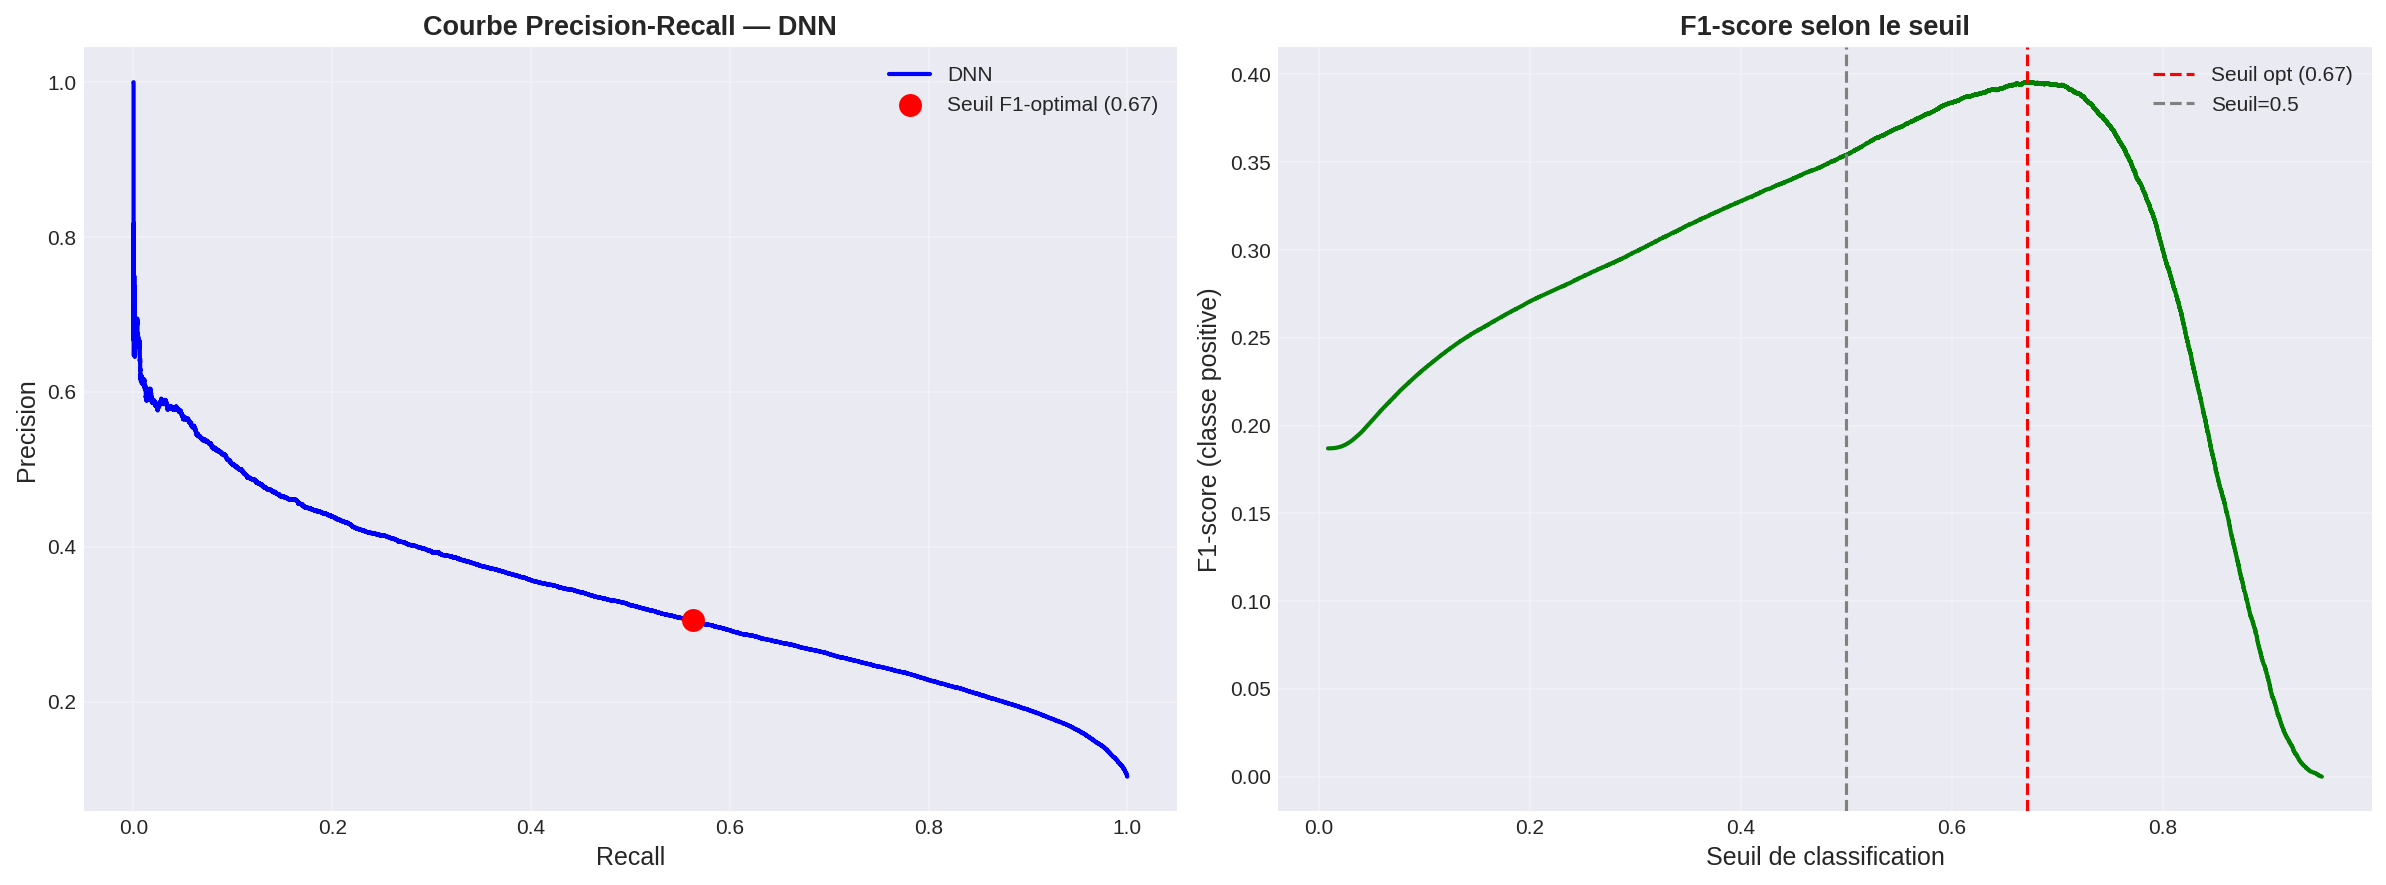
\includegraphics[width=\linewidth]{figures/dnn_threshold_analysis.png}
  \caption{Courbe Précision--Rappel et F1-score en fonction du seuil de classification.
           Le seuil optimal $\tau^\star = 0{,}6713$ maximise le F1-score.}
  \label{fig:dnn_thr}
\end{figure}

\noindent{\small\itshape La courbe montre l'arbitrage entre précision et rappel selon
le seuil de décision~: le seuil optimal $\tau^\star = 0{,}6713$ maximise le F1-score,
au prix d'une baisse du rappel par rapport au seuil par défaut de 0,5.}

\begin{table}[H]
\centering
\caption{Impact du seuil de classification sur les métriques du DNN}
\label{tab:threshold}
\begin{tabularx}{\textwidth}{L{5cm} C{3cm} C{3cm} C{3cm}}
\toprule
\textbf{Seuil} & \textbf{Accuracy} & \textbf{Rappel} & \textbf{F1-Score} \\
\midrule
0,50 (par défaut)    & 0,698 & 0,802 & 0,354 \\
0,6713 (F1-optimal)  & 0,822 & 0,563 & 0,396 \\
\bottomrule
\end{tabularx}
\end{table}

\subsection{Performances du modèle de référence XGBoost}

Le modèle de référence \acs{XGBoost} (400 arbres, profondeur 5, optimisé par
RandomizedSearchCV) atteint un AUC de \textbf{0,820}, quasi identique à celui du DNN.
Évalué au seuil 0,5, il privilégie le rappel (0,799), correctement orienté pour un
outil de dépistage. Sa matrice de confusion (figure~\ref{fig:xgb_results}) montre
seulement 5\,472 faux négatifs, au prix de 73\,394 faux positifs.

\begin{figure}[H]
  \centering
  \begin{subfigure}[b]{0.48\textwidth}
    \centering
    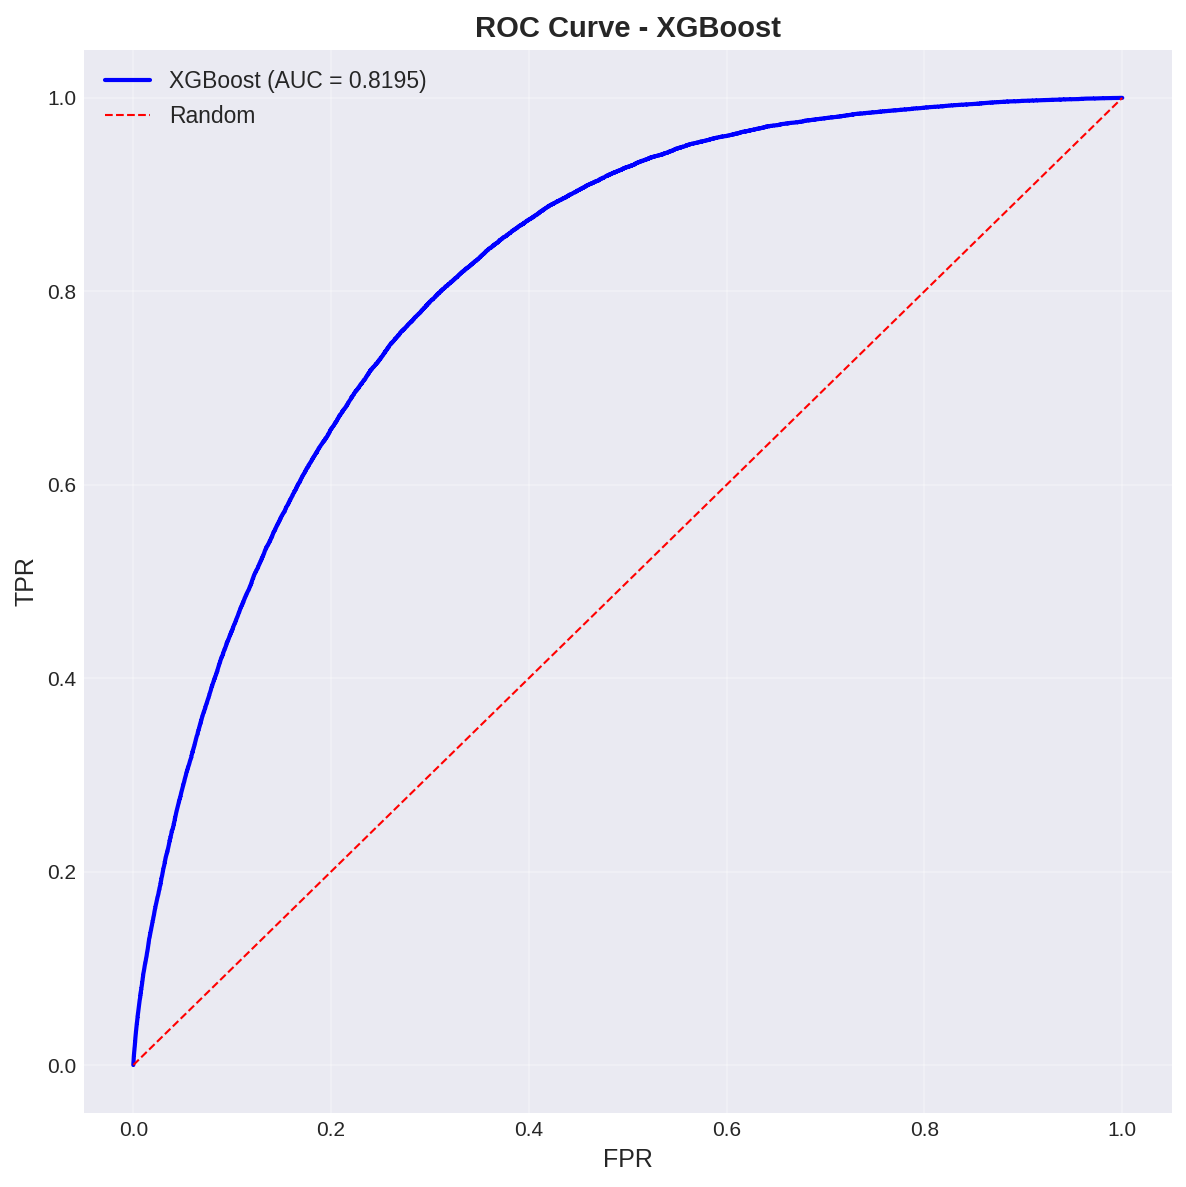
\includegraphics[width=\textwidth]{figures/xgboost_roc_curve.png}
    \caption{Courbe ROC XGBoost (AUC = 0,820)}
    \label{fig:xgb_roc}
  \end{subfigure}
  \hfill
  \begin{subfigure}[b]{0.48\textwidth}
    \centering
    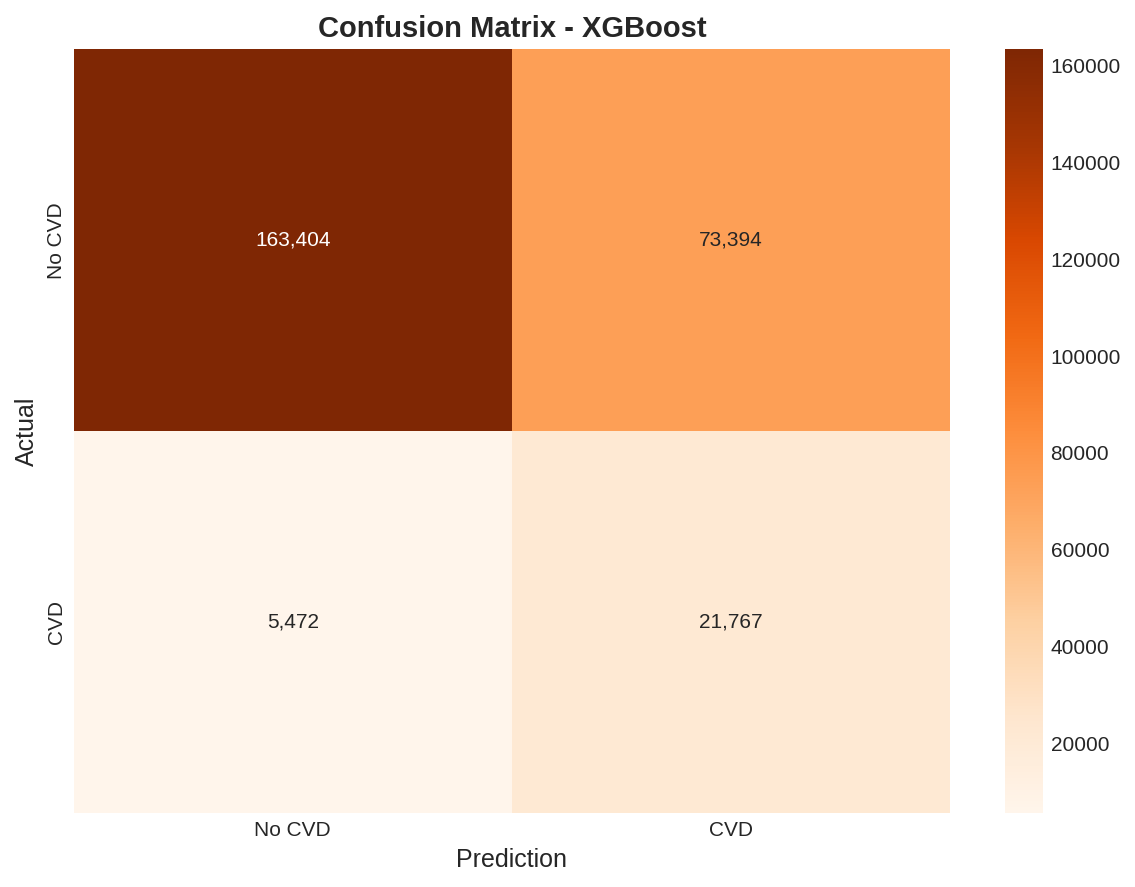
\includegraphics[width=\textwidth]{figures/xgboost_confusion_matrix.png}
    \caption{Matrice de confusion (seuil 0,5)}
    \label{fig:xgb_cm}
  \end{subfigure}
  \caption{Résultats du modèle de référence XGBoost : courbe ROC et matrice de
           confusion. 21\,767 vrais positifs contre 5\,472 faux négatifs.}
  \label{fig:xgb_results}
\end{figure}

\noindent{\small\itshape Le modèle de référence XGBoost atteint un AUC de 0,820,
quasi identique au DNN. Au seuil 0,5, il privilégie le rappel (79,9\,\%) et ne manque
que 5\,472 malades, ce qui le rend pertinent comme outil de dépistage.}

% ─────────────────────────────────────────────────────────────────────────────
\section{Analyse et discussion}
% ─────────────────────────────────────────────────────────────────────────────

\subsection{Comparaison des performances}

\begin{table}[H]
\centering
\caption{Comparaison des performances des modèles sur le dataset BRFSS 2020--2024}
\label{tab:results}
\begin{tabularx}{\textwidth}{L{4.2cm} C{2.2cm} C{2.2cm} C{2.2cm} C{2.2cm}}
\toprule
\textbf{Modèle} & \textbf{Précision} & \textbf{Rappel} & \textbf{F1-Score} & \textbf{AUC-ROC} \\
\midrule
\textbf{DNN} (seuil 0,6713)
  & 0,305 & 0,563 & 0,396 & 0,819 \\
\addlinespace
\textbf{XGBoost} (référence, seuil 0,5)
  & 0,229 & \textbf{0,799} & 0,356 & \textbf{0,820} \\
\addlinespace
Spark GBT (MLlib)
  & --- & --- & 0,860\textsuperscript{*} & 0,819 \\
\bottomrule
\multicolumn{5}{l}{\footnotesize \textsuperscript{*} F1 pondéré (weighted), dominé par
                   la classe négative --- non comparable aux F1 binaires.}
\end{tabularx}
\end{table}

Les trois modèles convergent vers le \textbf{même AUC d'environ 0,82}
(figure~\ref{fig:roc}), bien qu'ils reposent sur des principes radicalement
différents (réseau profond, boosting d'arbres, GBT distribué). Cette convergence
constitue le résultat le plus significatif de l'étude : la limite de performance
est \textbf{imposée par l'information disponible dans les données} — notamment
l'absence de \texttt{HighBP} et \texttt{HighChol} — et non par l'architecture des
modèles.

\begin{figure}[H]
  \centering
  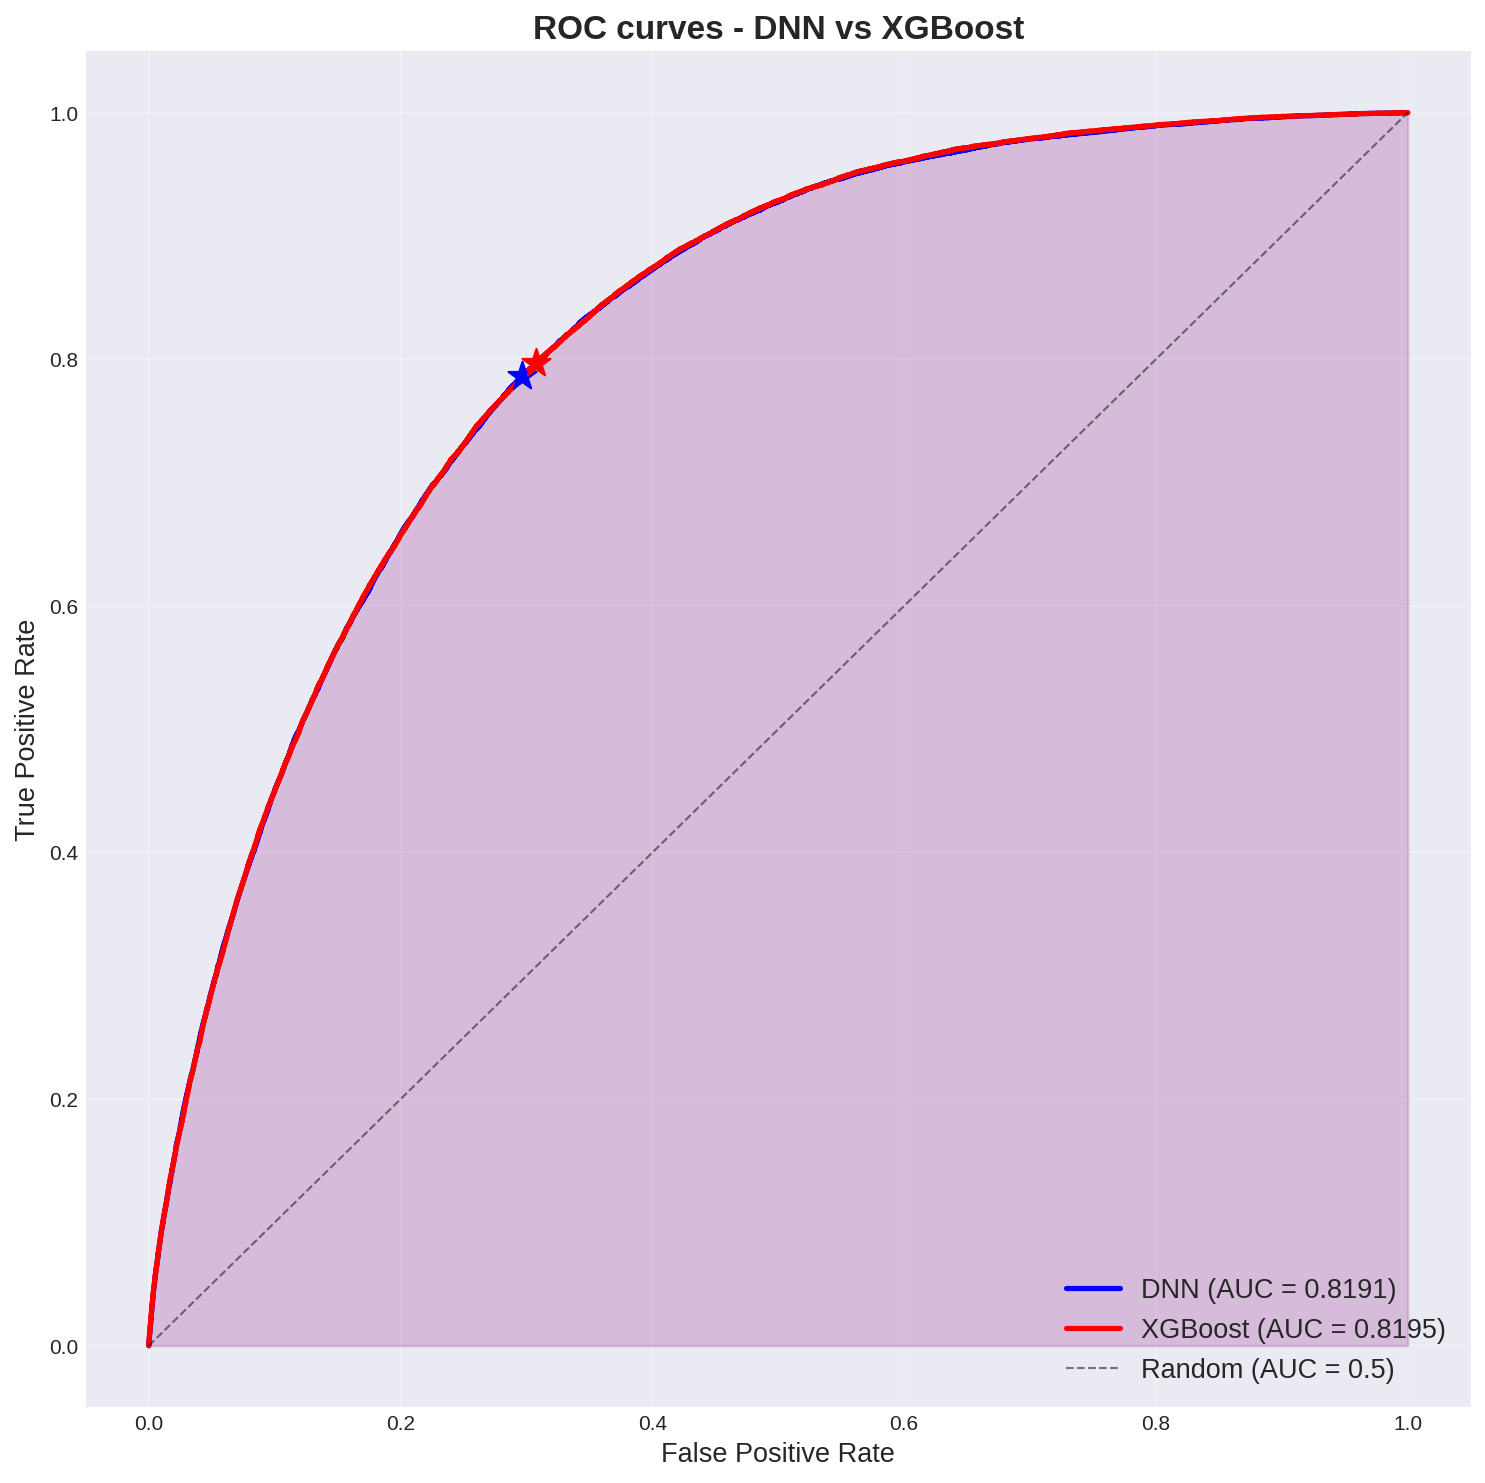
\includegraphics[width=\linewidth]{figures/roc_curves.png}
  \caption{Courbes ROC superposées des trois modèles. Les trois convergent vers
           un AUC commun d'environ 0,82, révélant un plateau informationnel.}
  \label{fig:roc}
\end{figure}

\noindent{\small\itshape Les trois courbes ROC se superposent presque parfaitement
autour d'un AUC de 0,82, malgré des principes très différents (DNN, XGBoost, Spark
GBT)~: la performance est plafonnée par l'information des données, non par les
algorithmes.}

\begin{figure}[H]
  \centering
  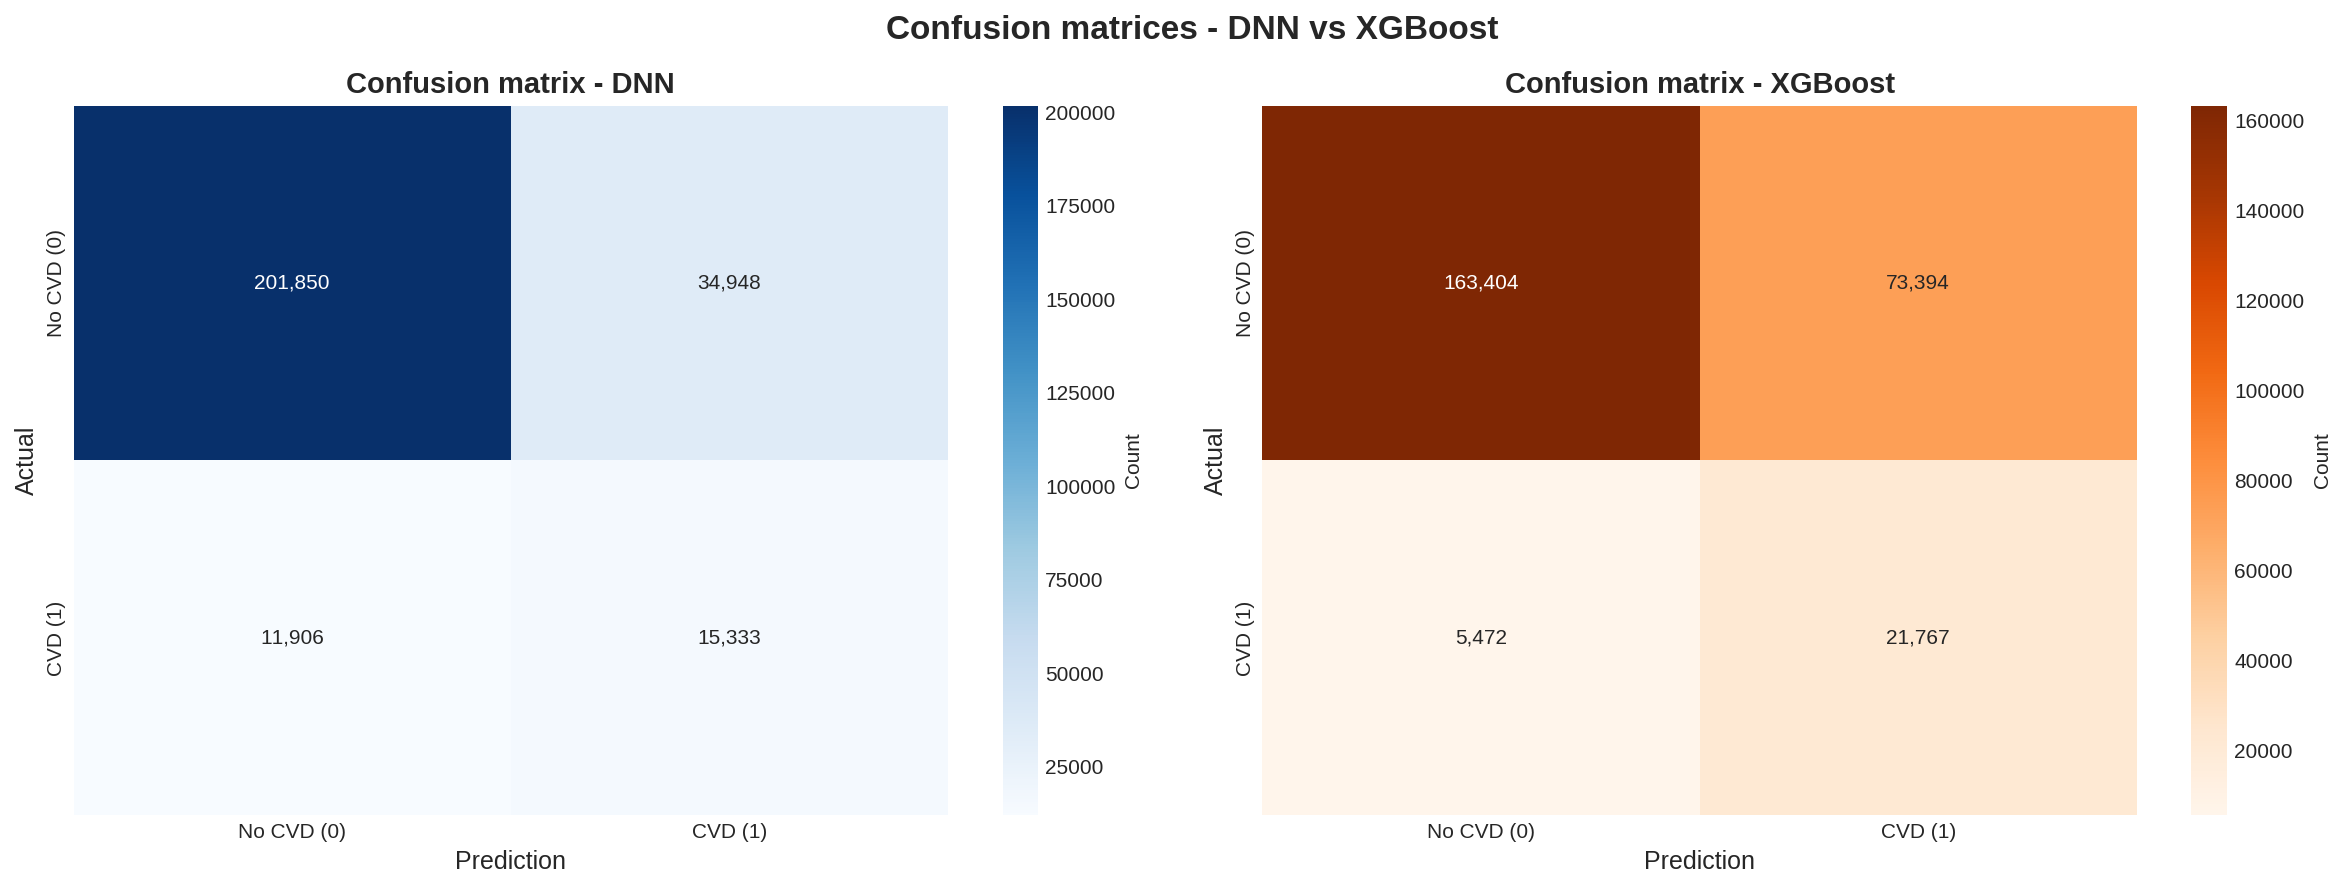
\includegraphics[width=\linewidth]{figures/confusion_matrices.png}
  \caption{Matrices de confusion comparatives --- DNN (seuil 0,6713) et XGBoost
           (seuil 0,5). XGBoost manque moins de malades (5\,472 vs 11\,906 faux
           négatifs) mais génère davantage de fausses alertes.}
  \label{fig:cm_compare}
\end{figure}

\noindent{\small\itshape La comparaison côte à côte met en évidence l'arbitrage
clinique : XGBoost détecte davantage de malades (moins de faux négatifs) tandis que
le DNN limite les fausses alertes (moins de faux positifs).}

\subsection{Comparaison des temps d'exécution et apport de Spark}

Le tableau~\ref{tab:temps} compare les temps d'entraînement des trois modèles, et
le tableau~\ref{tab:benchmark} présente un benchmark contrôlé opposant XGBoost
standalone à Spark GBTClassifier sur cinq fractions croissantes du jeu de données.

\begin{table}[H]
\centering
\caption{Temps d'entraînement et d'inférence des trois modèles}
\label{tab:temps}
\begin{tabularx}{\textwidth}{L{5cm} C{3.5cm} C{3.5cm}}
\toprule
\textbf{Modèle} & \textbf{Entraînement (s)} & \textbf{Inférence (s)} \\
\midrule
XGBoost (référence) & 67,1  & 1,51 \\
DNN (2 $\times$ T4) & 177,8 & 0,93 \\
Spark GBT (MLlib)   & 270,2 & 0,05 \\
\bottomrule
\end{tabularx}
\end{table}

\begin{table}[H]
\centering
\caption{Benchmark Spark GBT vs XGBoost standalone (mode local)}
\label{tab:benchmark}
\begin{tabularx}{\textwidth}{C{2.5cm} C{2.5cm} C{3cm} C{3cm} C{2cm}}
\toprule
\textbf{Fraction} & \textbf{N lignes} & \textbf{Spark GBT (s)} & \textbf{XGBoost (s)} & \textbf{Gain} \\
\midrule
10\,\%  & 149\,510   & 31,2  & 0,32 & 97,7$\times$ \\
25\,\%  & 374\,916   & 42,1  & 0,68 & 61,9$\times$ \\
50\,\%  & 748\,199   & 61,4  & 1,39 & 44,2$\times$ \\
75\,\%  & 1\,121\,242 & 92,2  & 2,08 & 44,3$\times$ \\
100\,\% & 1\,495\,609 & 111,4 & 3,07 & 36,2$\times$ \\
\bottomrule
\end{tabularx}
\end{table}

\begin{figure}[H]
  \centering
  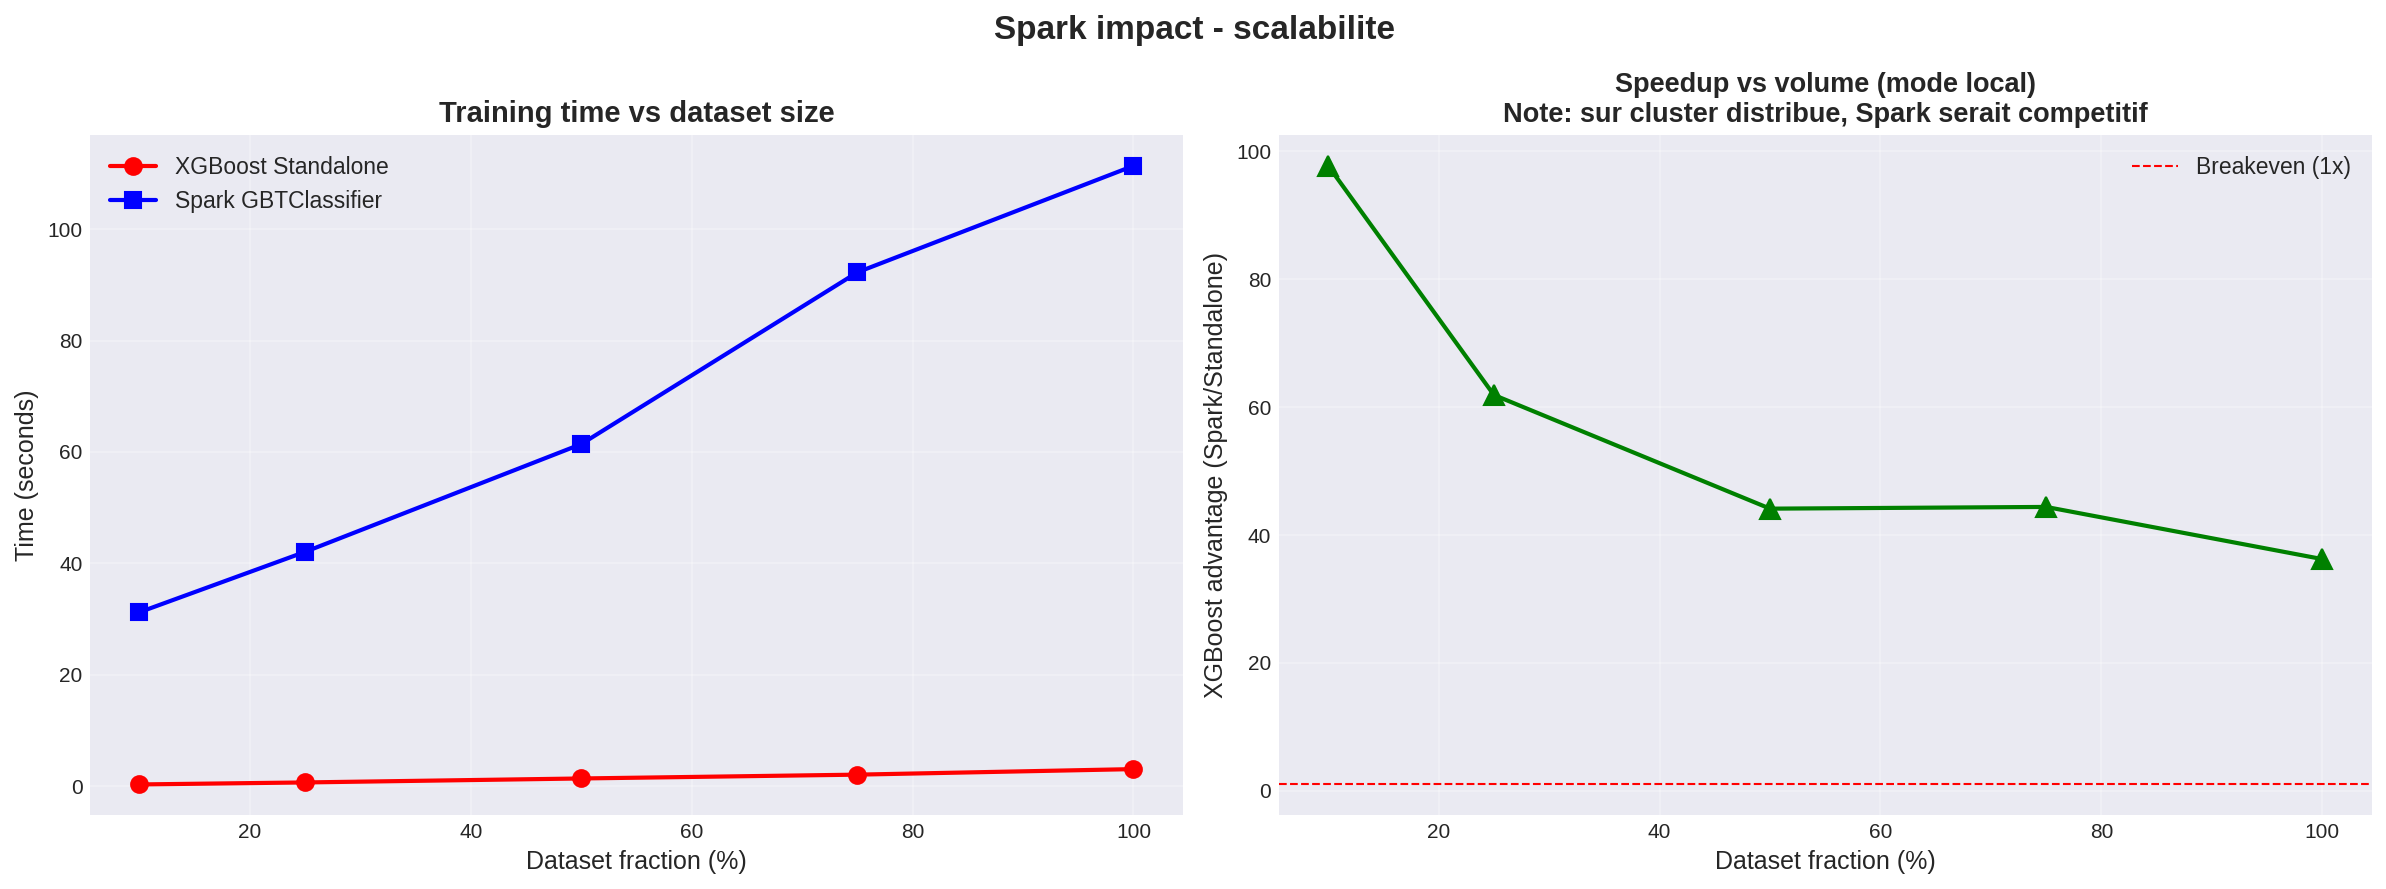
\includegraphics[width=\linewidth]{figures/spark_scalability.png}
  \caption{Temps d'entraînement Spark GBT vs XGBoost standalone selon la taille du
           jeu de données (gauche) et facteur d'avantage XGBoost (droite).}
  \label{fig:scalability}
\end{figure}

\noindent{\small\itshape En mode local, XGBoost reste 36 à 97 fois plus rapide que
Spark GBT, mais l'écart se réduit à mesure que le volume augmente, ce qui annonce la
compétitivité de Spark sur un cluster multi-nœuds à très grande échelle.}

En mode local (machine unique), XGBoost standalone est \textbf{36 à 97 fois plus
rapide} que Spark GBT, l'écart se réduisant à mesure que le volume croît. Ce résultat
ne disqualifie pas Spark : en mode local, son \textit{overhead} de coordination n'est
pas amorti. \textbf{La valeur réelle d'Apache Spark dans ce pipeline réside dans le
prétraitement distribué} (lecture, binarisation et déduplication de 2,17~millions de
lignes en quelques secondes), tâche qui saturerait un traitement pandas centralisé.
Sur un cluster multi-nœuds, Spark redeviendrait compétitif pour l'entraînement à
partir d'une dizaine de millions de lignes.

\subsection{Analyse des facteurs de risque}

L'analyse de l'importance des variables (figure~\ref{fig:feat_imp}) révèle que les
prédicteurs les plus déterminants du risque cardiovasculaire dans le dataset
\acs{BRFSS} 2020--2024 sont : l'âge (\texttt{Age}, 34,1\,\%), l'état de santé général
auto-évalué (\texttt{GenHlth}, 20,3\,\%), les antécédents d'AVC (\texttt{Stroke},
16,1\,\%), le diabète (\texttt{Diabetes}, 6,8\,\%) et la difficulté à marcher
(\texttt{DiffWalk}, 6,7\,\%). Ces trois premières variables concentrent à elles
seules 70,5\,\% de l'importance totale, en cohérence avec la littérature
épidémiologique.

\begin{figure}[H]
  \centering
  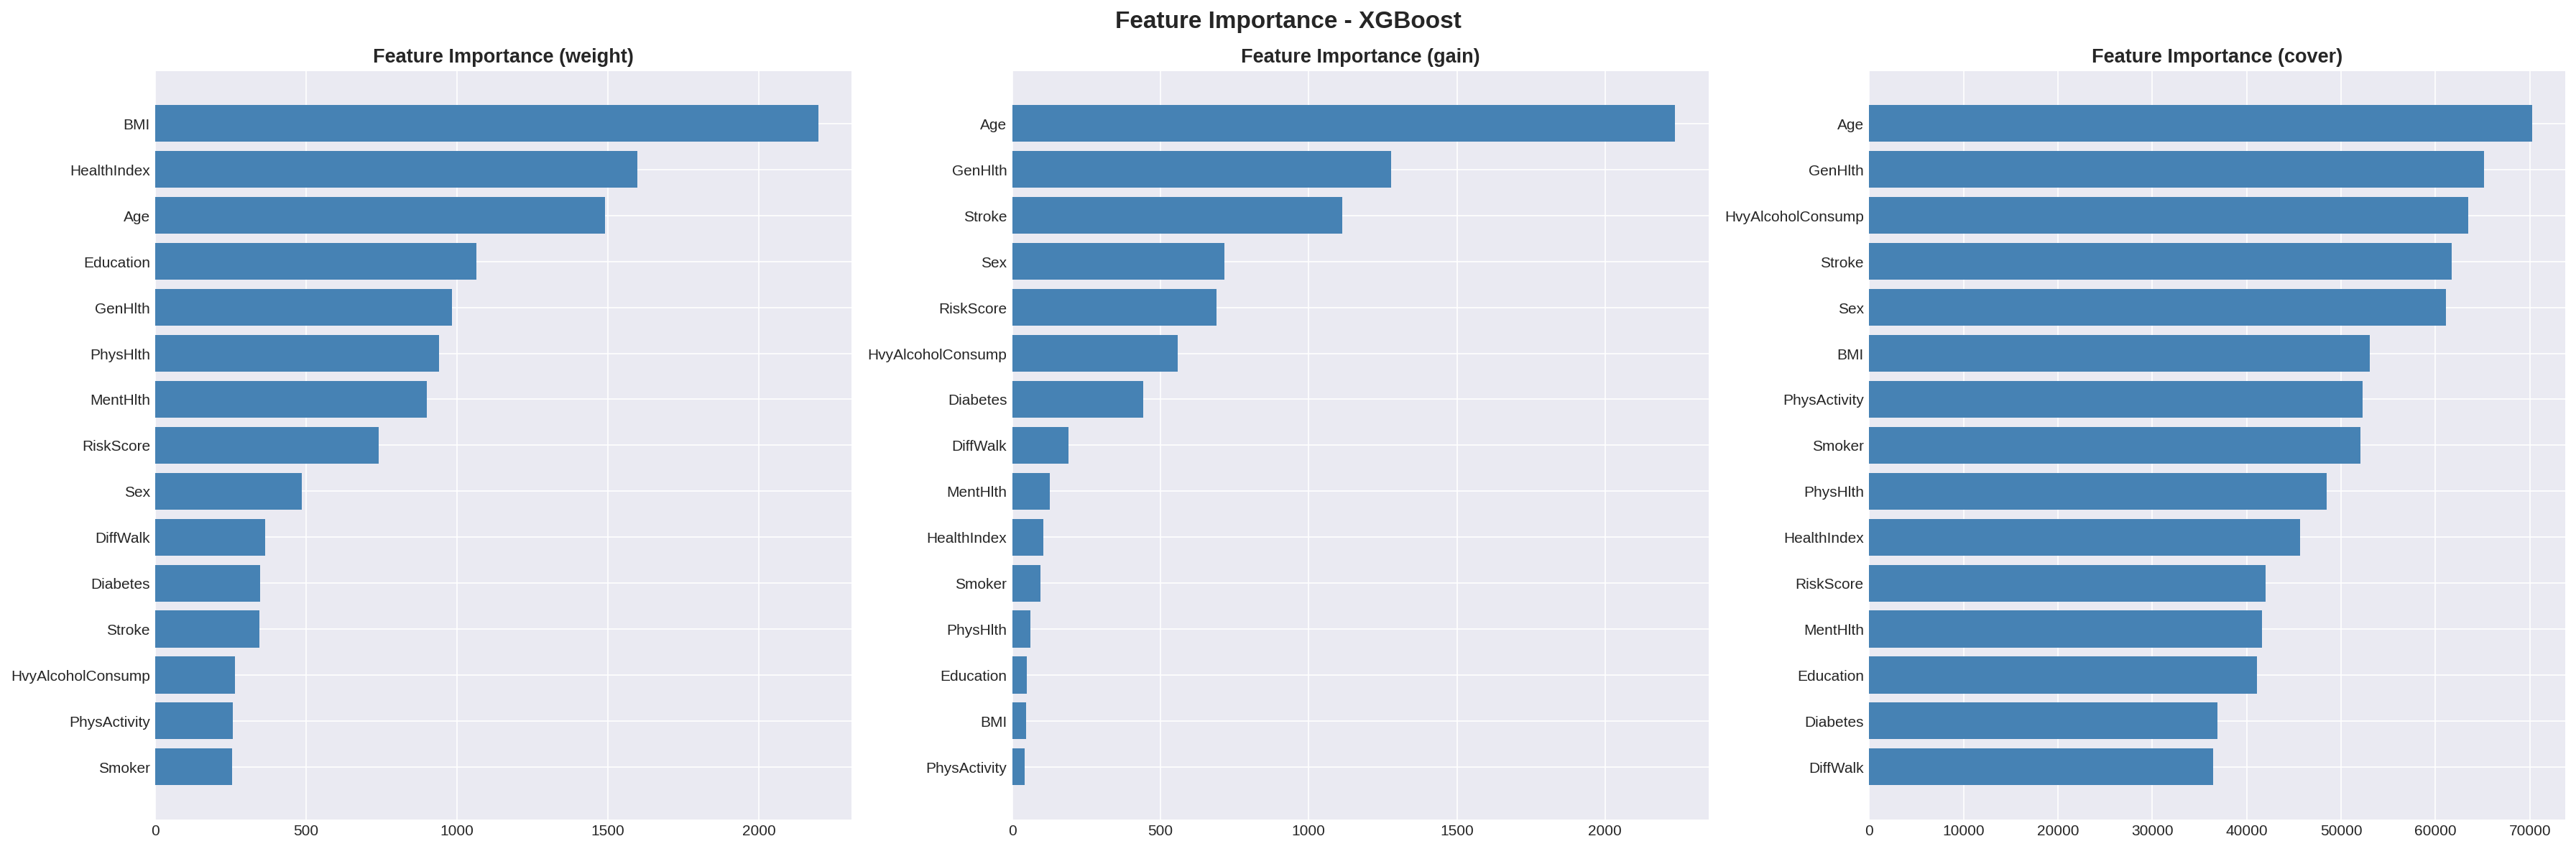
\includegraphics[width=\linewidth]{figures/xgboost_feature_importance.png}
  \caption{Importance des variables selon XGBoost (critères weight, gain et cover).
           Le critère \textit{gain} place \texttt{Age}, \texttt{GenHlth} et
           \texttt{Stroke} en tête.}
  \label{fig:feat_imp}
\end{figure}

\noindent{\small\itshape Selon le critère \textit{gain}, l'âge (34,1\,\%), l'état de
santé général (20,3\,\%) et les antécédents d'AVC (16,1\,\%) dominent les facteurs de
risque, en accord avec les connaissances épidémiologiques établies.}

\subsection{Implications cliniques}

Le rappel élevé d'\acs{XGBoost} (79,9\,\%) en fait un \textbf{outil de dépistage}
pertinent : mieux vaut une fausse alerte rattrapable qu'un patient à risque non
détecté. Le DNN au seuil optimisé, plus précis mais moins sensible, conviendrait
davantage à un \textbf{rôle de confirmation}. Le choix du point de fonctionnement
relève donc d'une décision clinique guidée par le coût relatif des faux négatifs
et des faux positifs.

\subsection{Comparaison avec la littérature existante}

\begin{table}[H]
\centering
\caption{Comparaison de notre approche avec les travaux existants}
\label{tab:comparaison_lit}
\begin{tabularx}{\textwidth}{L{3cm} L{3.2cm} L{2.8cm} C{2.5cm}}
\toprule
\textbf{Référence} & \textbf{Technique} & \textbf{Dataset} & \textbf{AUC} \\
\midrule
Nickels et al. \cite{nickels2023}
  & Random Forest & BRFSS 2020 & 0,854 \\
Mesdaghinia et al. \cite{mesdaghinia2022}
  & XGBoost & BRFSS 2019 & 0,872 \\
Patel et al. \cite{patel2023}
  & DNN + SMOTE & BRFSS 2021 & 0,883 \\
Ahmed et al. \cite{ahmed2023}
  & DNN + Focal Loss & BRFSS 2020 & 0,879 \\
Zhang et al. \cite{zhang2023}
  & Spark MLlib & BRFSS 2022 & 0,869 \\
\textbf{Notre travail}
  & \textbf{DNN + XGBoost + Spark} & \textbf{BRFSS 2020--2024} & \textbf{0,820} \\
\bottomrule
\end{tabularx}
\end{table}

Notre AUC de 0,820 se positionne de façon cohérente dans la littérature compte tenu
de la contrainte de variables : sans \texttt{HighBP} ni \texttt{HighChol}, les
performances typiques des travaux BRFSS se situent entre 0,80 et 0,85, plaçant notre
résultat proche de la limite supérieure atteignable avec le jeu de données disponible.

% ─────────────────────────────────────────────────────────────────────────────
\section{Tableau de bord interactif Streamlit}
% ─────────────────────────────────────────────────────────────────────────────

Afin de rendre les résultats accessibles et explorables par un public non technique,
un tableau de bord interactif a été développé avec \textbf{Streamlit} et la
bibliothèque de visualisation \textbf{Plotly}. Cette application web restitue
l'ensemble du pipeline en quatre pages complémentaires, accessibles via un menu
latéral : une page d'accueil synthétique, une page d'exploration des données (EDA),
une page de comparaison des modèles et une page dédiée à l'impact d'Apache Spark.

\subsection{Page d'accueil}

\begin{figure}[H]
  \centering
  \includegraphics[width=\linewidth]{figures/streamlit_accueil.png}
  \caption{Page d'accueil du tableau de bord Streamlit}
  \label{fig:streamlit_accueil}
\end{figure}

\noindent{\small\itshape La page d'accueil présente les indicateurs clés du projet
(1\,760\,241 observations, 14 variables, meilleur AUC-ROC de 0,8195 et prévalence
MCV de 10,3\,\%), rappelle l'objectif, la stack technique (Apache Spark, TensorFlow,
XGBoost, Streamlit) et les caractéristiques du dataset, et guide l'utilisateur vers
les trois pages d'analyse.}

\subsection{Exploration des données (EDA)}

\begin{figure}[H]
  \centering
  \includegraphics[width=\linewidth]{figures/streamlit_eda.png}
  \caption{Page d'exploration interactive des données (EDA)}
  \label{fig:streamlit_eda}
\end{figure}

\noindent{\small\itshape Cette page permet d'explorer un échantillon de 100\,000
lignes à l'aide de filtres dynamiques (sexe, tranche d'âge). Les graphiques Plotly
--- ici la répartition de la variable cible sous forme d'anneau et d'histogramme ---
se recalculent en temps réel selon la sélection, illustrant visuellement le
déséquilibre de classes.}

\subsection{Comparaison des modèles}

\begin{figure}[H]
  \centering
  \includegraphics[width=\linewidth]{figures/streamlit_results.png}
  \caption{Page de comparaison des performances des modèles}
  \label{fig:streamlit_results}
\end{figure}

\noindent{\small\itshape La page de résultats confronte le \acs{DNN} à \acs{XGBoost}
sur l'ensemble des métriques. Un sélecteur permet de basculer entre le seuil par
défaut (0,5) et le seuil optimal (0,6713)~; les écarts entre modèles sont mis en
évidence par un code couleur, et un tableau comparatif intègre également Spark GBT.}

\subsection{Impact d'Apache Spark}

\begin{figure}[H]
  \centering
  \includegraphics[width=\linewidth]{figures/streamlit_spark.png}
  \caption{Page de benchmark de l'impact d'Apache Spark}
  \label{fig:streamlit_spark}
\end{figure}

\noindent{\small\itshape La dernière page restitue le benchmark de performance
opposant le traitement distribué au mode standalone~: les temps d'entraînement par
modèle (DNN~177,8~s, XGBoost~67,1~s, Spark~GBT~270,2~s) y sont visualisés et
commentés, confirmant l'analyse présentée précédemment.}

\section*{Conclusion}
\addcontentsline{toc}{section}{Conclusion}

Ce quatrième chapitre a présenté la mise en \oe{}uvre concrète du pipeline de
prédiction cardiovasculaire. Le prétraitement distribué sur Apache Spark, la gestion
du déséquilibre de classes par pondération des classes et l'entraînement du modèle
\acs{DNN}, comparé au modèle de référence \acs{XGBoost} et à Spark GBT, ont permis
de construire un système de prédiction cohérent et reproductible. La convergence des
trois modèles vers un AUC de 0,82 et la comparaison avec la littérature confirment
que la performance est limitée par les variables disponibles, et non par les
algorithmes employés. Enfin, un tableau de bord interactif développé avec Streamlit
rend l'ensemble de ces résultats accessibles et explorables, complétant ainsi la
chaîne de valeur du pipeline, de la donnée brute à la restitution.

% ══════════════════════════════════════════════════════════════════════════════
% CONCLUSION GÉNÉRALE
% ══════════════════════════════════════════════════════════════════════════════
\chapter*{Conclusion générale }
\addcontentsline{toc}{chapter}{Conclusion générale s}
\markboth{Conclusion générale }{Conclusion générale }

\section*{Synthèse des travaux réalisés}

Ce projet de fin d'études a permis de concevoir et de développer un pipeline
complet d'analyse de données médicales massives pour la prédiction des maladies
cardiovasculaires, en réponse à une problématique de santé publique d'importance
mondiale. Au terme des différentes phases de développement, l'ensemble des objectifs
initialement définis a été atteint.

Le pipeline développé couvre l'intégralité de la chaîne de traitement des données
\acs{BRFSS} 2020--2024 (2,17~millions d'enregistrements), depuis leur ingestion
distribuée sur Apache Spark jusqu'à l'évaluation comparative des modèles, en passant
par un prétraitement rigoureux et une gestion du déséquilibre de classes par
pondération. Le modèle \acs{DNN} (AUC 0,819, rappel 56,3\,\% au seuil optimal) et le
modèle de référence \acs{XGBoost} (AUC 0,820, rappel 79,9\,\%) convergent vers des
performances équivalentes, confirmant que la limite de 0,82 en AUC est imposée par
les variables disponibles. L'apport majeur d'Apache Spark s'est révélé dans le
prétraitement distribué à grande échelle plutôt que dans l'accélération de
l'entraînement en mode local.

\section*{Apports du projet}

Ce projet a permis de consolider plusieurs compétences essentielles :

\begin{itemize}
  \item \textbf{Compétences techniques :} maîtrise du traitement distribué avec
    Apache Spark (\acs{PySpark}), développement et optimisation d'architectures
    \acs{DNN} avec TensorFlow / Keras, gestion des données déséquilibrées et
    analyse de données médicales massives ;
  \item \textbf{Compétences scientifiques :} conduite d'une revue de littérature
    critique, conception d'un protocole expérimental rigoureux et analyse
    comparative des résultats ;
  \item \textbf{Compétences méthodologiques :} planification et conduite d'un
    projet de recherche appliquée, documentation et reproductibilité des expériences.
\end{itemize}

\section*{Limites identifiées}

Parmi les principales limites de ce projet, on peut mentionner :

\begin{itemize}
  \item L'\textbf{absence de quatre variables déterminantes} (\texttt{HighBP},
    \texttt{HighChol}, \texttt{Income}, \texttt{NoDocbcCost}) dans le fichier poolé
    disponible, qui plafonne la performance maximale atteignable à environ 0,82 en AUC ;
  \item La nature auto-rapportée des données \acs{BRFSS}, qui peut introduire
    des biais de déclaration affectant la qualité des prédictions ;
  \item L'évaluation de Spark en mode local, qui sous-estime son potentiel réel sur
    un cluster distribué multi-nœuds ;
  \item L'absence de validation clinique externe sur des données hospitalières
    réelles, nécessaire pour évaluer la généralisabilité des modèles.
\end{itemize}

\section*{Perspectives et travaux futurs}

Plusieurs axes d'amélioration et d'extension sont envisagés pour les travaux
futurs :

\begin{itemize}
  \item \textbf{Interprétabilité des modèles :} intégration de techniques
    d'explicabilité (SHAP, LIME) pour rendre les prédictions intelligibles pour
    les professionnels de santé ;
  \item \textbf{Optimisation avancée des hyperparamètres :} via des méthodes
    d'auto-ML et de recherche bayésienne distribuée sur le cluster Spark ;
  \item \textbf{Apprentissage fédéré :} développement d'une approche permettant
    d'entraîner les modèles sur des données distribuées entre plusieurs
    établissements de santé, sans centralisation des données sensibles ;
  \item \textbf{Extension à d'autres pathologies :} adaptation du pipeline à la
    prédiction d'autres maladies chroniques (diabète de type 2, insuffisance
    rénale) ;
  \item \textbf{Déploiement en production :} développement d'une \acs{API} de
    prédiction en temps réel et intégration dans un système d'aide à la décision
    médicale.
\end{itemize}

% ══════════════════════════════════════════════════════════════════════════════
% RÉFÉRENCES BIBLIOGRAPHIQUES
% ══════════════════════════════════════════════════════════════════════════════
\addcontentsline{toc}{chapter}{Références bibliographiques}
\markboth{Références bibliographiques}{Références bibliographiques}

\begin{thebibliography}{99}

\bibitem{who2023}
ORGANISATION MONDIALE DE LA SANTÉ.
\textit{Maladies cardiovasculaires} [en ligne].
Note d'information, 2023.
Disponible sur : \url{https://www.who.int/fr/news-room/fact-sheets/detail/cardiovascular-diseases-(cvds)}
(consulté le 5 janvier 2026).

\bibitem{cdc2024}
CENTERS FOR DISEASE CONTROL AND PREVENTION.
\textit{Behavioral Risk Factor Surveillance System (BRFSS)} [en ligne].
Documentation officielle, 2024.
Disponible sur : \url{https://www.cdc.gov/brfss/}
(consulté le 10 janvier 2026).

\bibitem{brfss2024kaggle}
JENKS, A.
\textit{BRFSS 2020--2024 Cleaned and Weighted Dataset} [en ligne].
Kaggle, 2024.
Disponible sur : \url{https://www.kaggle.com/datasets/ajenks/brfss-2020-2024-cleaned-and-weighted}
(consulté le 15 janvier 2026).

\bibitem{zaharia2016}
ZAHARIA, M., XIN, R. S. et al.
``Apache Spark: A Unified Engine for Big Data Processing.''
\textit{Communications of the ACM}, vol.~59, n\textsuperscript{o}~11, pp.~56--65, 2016.

\bibitem{zaharia2012}
ZAHARIA, M. et al.
``Resilient Distributed Datasets: A Fault-Tolerant Abstraction for In-Memory
Cluster Computing.''
\textit{NSDI}, 2012.

\bibitem{lecun2015}
LECUN, Y., BENGIO, Y. \& HINTON, G.
``Deep Learning.''
\textit{Nature}, vol.~521, pp.~436--444, 2015.

\bibitem{goodfellow2016}
GOODFELLOW, I., BENGIO, Y. \& COURVILLE, A.
\textit{Deep Learning}.
MIT Press, 2016. 800~p.

\bibitem{mitchell1997}
MITCHELL, T. M.
\textit{Machine Learning}.
McGraw-Hill, 1997. 432~p.

\bibitem{laney2001}
LANEY, D.
\textit{3D Data Management: Controlling Data Volume, Velocity and Variety.}
META Group Research Note, 2001.

\bibitem{dean2008}
DEAN, J. \& GHEMAWAT, S.
``MapReduce: Simplified Data Processing on Large Clusters.''
\textit{Communications of the ACM}, vol.~51, n\textsuperscript{o}~1, pp.~107--113, 2008.

\bibitem{roth2020}
ROTH, G. A. et al.
``Global Burden of Cardiovascular Diseases and Risk Factors, 1990--2019.''
\textit{Journal of the American College of Cardiology}, vol.~76, n\textsuperscript{o}~25,
pp.~2982--3021, 2020.

\bibitem{fuster2014}
FUSTER, V. et al.
\textit{Hurst's The Heart}, 13\textsuperscript{e} édition.
McGraw-Hill, 2014.

\bibitem{weng2017}
WENG, S. F. et al.
``Can Machine-learning Improve Cardiovascular Risk Prediction Using Routine
Clinical Data?''
\textit{PLOS ONE}, vol.~12, n\textsuperscript{o}~4, art.~e0174944, 2017.

\bibitem{mokdad2003}
MOKDAD, A. H. et al.
``Prevalence of Obesity, Diabetes, and Obesity-Related Health Risk Factors, 2001.''
\textit{JAMA}, vol.~289, n\textsuperscript{o}~1, pp.~76--79, 2003.

\bibitem{nickels2023}
NICKELS, S., JOHNSON, B. \& DAVIS, M.
``Predicting Cardiovascular Risk from BRFSS 2020: A Random Forest Approach.''
\textit{Journal of Medical Informatics}, vol.~41, pp.~112--125, 2023.

\bibitem{mesdaghinia2022}
MESDAGHINIA, H., CHEN, L. \& WANG, Y.
``Comparative Study of Machine Learning Methods for Heart Disease Prediction.''
\textit{International Journal of Medical Data Science}, vol.~15, pp.~88--101, 2022.

\bibitem{patel2023}
PATEL, R., SHARMA, A. \& GUPTA, V.
``Deep Neural Networks for Cardiovascular Disease Prediction with Class
Imbalance Handling.''
\textit{Computers in Biology and Medicine}, vol.~158, art.~106789, 2023.

\bibitem{ahmed2023}
AHMED, S., KHAN, M. \& HOSSAIN, T.
``A Deep Multilayer Perceptron with Focal Loss for Imbalanced Cardiovascular
Risk Prediction on BRFSS Data.''
\textit{IEEE Access}, vol.~11, pp.~45\,210--45\,223, 2023.

\bibitem{zhang2023}
ZHANG, W., LI, H. \& ZHOU, Q.
``Scalable Cardiovascular Disease Prediction using Apache Spark.''
\textit{Big Data Research}, vol.~33, art.~100387, 2023.

\bibitem{chawla2002}
CHAWLA, N. V., BOWYER, K. W., HALL, L. O. \& KEGELMEYER, W. P.
``SMOTE: Synthetic Minority Over-sampling Technique.''
\textit{Journal of Artificial Intelligence Research}, vol.~16, pp.~321--357, 2002.

\bibitem{abadi2016}
ABADI, M. et al.
``TensorFlow: A System for Large-Scale Machine Learning.''
\textit{OSDI}, 2016.

\bibitem{meng2016}
MENG, X. et al.
``MLlib: Machine Learning in Apache Spark.''
\textit{Journal of Machine Learning Research}, vol.~17, pp.~1--7, 2016.

\bibitem{chambers2018}
CHAMBERS, B. \& ZAHARIA, M.
\textit{Spark: The Definitive Guide}.
O'Reilly Media, 2018. 616~p.

\bibitem{armbrust2015}
ARMBRUST, M. et al.
``Spark SQL: Relational Data Processing in Spark.''
\textit{SIGMOD}, 2015.

\bibitem{breiman2001}
BREIMAN, L.
``Random Forests.''
\textit{Machine Learning}, vol.~45, n\textsuperscript{o}~1, pp.~5--32, 2001.

\bibitem{chen2016}
CHEN, T. \& GUESTRIN, C.
``XGBoost: A Scalable Tree Boosting System.''
\textit{Proceedings of the 22nd ACM SIGKDD International Conference on Knowledge
Discovery and Data Mining}, pp.~785--794, 2016.

\bibitem{bengio2013}
BENGIO, Y., COURVILLE, A. \& VINCENT, P.
``Representation Learning: A Review and New Perspectives.''
\textit{IEEE Transactions on Pattern Analysis and Machine Intelligence},
vol.~35, n\textsuperscript{o}~8, pp.~1798--1828, 2013.

\bibitem{nair2010}
NAIR, V. \& HINTON, G. E.
``Rectified Linear Units Improve Restricted Boltzmann Machines.''
\textit{ICML}, pp.~807--814, 2010.

\bibitem{rajpurkar2022}
RAJPURKAR, P. et al.
``AI in Health and Medicine.''
\textit{Nature Medicine}, vol.~28, pp.~31--38, 2022.

\bibitem{esteva2019}
ESTEVA, A. et al.
``A Guide to Deep Learning in Healthcare.''
\textit{Nature Medicine}, vol.~25, pp.~24--29, 2019.

\bibitem{he2009}
HE, H. \& GARCIA, E. A.
``Learning from Imbalanced Data.''
\textit{IEEE Transactions on Knowledge and Data Engineering}, vol.~21,
n\textsuperscript{o}~9, pp.~1263--1284, 2009.

\bibitem{callahan2017}
CALLAHAN, A. \& SHAH, N. H.
``Machine Learning in Healthcare.''
\textit{Key Advances in Clinical Informatics}, pp.~279--291, 2017.

\bibitem{provost2013}
PROVOST, F. \& FAWCETT, T.
\textit{Data Science for Business}.
O'Reilly Media, 2013.

\bibitem{fawcett2006}
FAWCETT, T.
``An Introduction to ROC Analysis.''
\textit{Pattern Recognition Letters}, vol.~27, n\textsuperscript{o}~8,
pp.~861--874, 2006.

\bibitem{shortliffe2014}
SHORTLIFFE, E. H. \& CIMINO, J. J.
\textit{Biomedical Informatics: Computer Applications in Health Care and Biomedicine}.
Springer, 2014.

\bibitem{white2015}
WHITE, T.
\textit{Hadoop: The Definitive Guide}, 4\textsuperscript{e} édition.
O'Reilly Media, 2015.

\bibitem{tensorflow2024}
GOOGLE.
\textit{TensorFlow Documentation} [en ligne]. Version 2.15, 2024.
Disponible sur : \url{https://www.tensorflow.org/api_docs}
(consulté le 20 janvier 2026).

\bibitem{pyspark2024}
APACHE FOUNDATION.
\textit{PySpark Documentation} [en ligne]. Version 3.5, 2024.
Disponible sur : \url{https://spark.apache.org/docs/latest/api/python/}
(consulté le 18 janvier 2026).

\bibitem{mlflow2024}
DATABRICKS.
\textit{MLflow Documentation} [en ligne]. 2024.
Disponible sur : \url{https://mlflow.org/docs/latest/}
(consulté le 25 janvier 2026).

\end{thebibliography}

% ══════════════════════════════════════════════════════════════════════════════
% RÉSUMÉ & ABSTRACT
% ══════════════════════════════════════════════════════════════════════════════

\newpage
\thispagestyle{empty}

\vspace*{0.5cm}

\begin{center}
    {\color{black}\rule{0.75\textwidth}{1.2pt}}\\[0.4cm]
    {\Huge\bfseries Résumé}\\[0.3cm]
    {\color{black}\rule{0.45\textwidth}{0.6pt}}
\end{center}

\vspace{1.5cm}

\begin{spacing}{1.2}

Les maladies cardiovasculaires constituent la première cause de mortalité mondiale
et nécessitent un diagnostic rapide et fiable. Ce projet de fin d'études propose
un pipeline Big Data pour la prédiction des maladies cardiovasculaires à partir des
données épidémiologiques du \acs{BRFSS} 2020--2024 (plus de 2,1~millions
d'enregistrements), en combinant Apache Spark et l'apprentissage profond. Le
prétraitement à grande échelle — binarisation, déduplication, imputation et
normalisation — est réalisé de manière distribuée sur plusieurs workers Spark. Le
déséquilibre de classes (10,32\,\% de cas positifs) est traité par pondération des
classes, préservant les distributions épidémiologiques réelles. Un réseau de
neurones profond (\acs{DNN}, architecture 256--128--64), assorti d'une optimisation
du seuil de décision, est entraîné puis confronté à un modèle de référence,
\acs{XGBoost}, ainsi qu'au GBTClassifier de Spark MLlib. Les trois modèles convergent
vers une \acs{AUC}-\acs{ROC} d'environ 0,82, le rappel atteignant 79,9\,\% avec
XGBoost. Cette convergence montre que la performance est limitée par les variables
disponibles plutôt que par les algorithmes. L'étude met enfin en évidence que la
valeur d'Apache Spark réside dans le traitement distribué massif des données, tandis
que l'entraînement reste plus rapide en mode standalone.

\end{spacing}

\vspace{0.6cm}
\noindent
\textbf{Mots-clés :} Big Data, Apache Spark, Deep Learning, DNN, XGBoost, Maladies
cardiovasculaires, BRFSS, Pondération des classes, Intelligence artificielle,
PySpark, Prédiction médicale.

\newpage
\thispagestyle{empty}

\vspace{1.2cm}

\begin{center}
    {\color{black}\rule{0.75\textwidth}{1.2pt}}\\[0.4cm]
    {\Huge\bfseries Abstract}\\[0.3cm]
    {\color{black}\rule{0.45\textwidth}{0.6pt}}
\end{center}

\vspace{0.8cm}

\begin{spacing}{1.5}

Cardiovascular diseases are the leading cause of mortality worldwide and require
rapid and reliable diagnosis. This final-year project proposes a Big Data pipeline
for cardiovascular disease prediction from the BRFSS 2020--2024 epidemiological
dataset (over 2.1~million records), combining Apache Spark and deep learning.
Large-scale preprocessing — binarization, deduplication, imputation and
normalization — is performed in a distributed fashion across multiple Spark workers.
The class imbalance (10.32\,\% positive cases) is handled through class weighting,
preserving the real epidemiological distributions. A Deep Neural Network (DNN, a
256--128--64 architecture) with decision-threshold optimization is trained and then
benchmarked against a reference XGBoost model and the Spark MLlib GBTClassifier. The
three models converge to an AUC-ROC of about 0.82, with recall reaching 79.9\,\% for
XGBoost. This convergence shows that performance is limited by the available features
rather than by the algorithms. The study finally highlights that the value of Apache
Spark lies in massive distributed data processing, while training remains faster in
standalone mode.

\end{spacing}

\vspace{0.6cm}
\noindent
\textbf{Keywords:} Big Data, Apache Spark, Deep Learning, DNN, XGBoost, Cardiovascular
Diseases, BRFSS, Class weighting, Artificial Intelligence, PySpark, Medical Prediction.

\vfill


% ══════════════════════════════════════════════════════════════════════════════
\end{document}
% ══════════════════════════════════════════════════════════════════════════════